%%%%%%%%%%%%%%%%%%%%%%%%%%%%%%%%%%%%%%%%%12pt: grandezza carattere
                                        %a4paper: formato a4
                                        %openright: apre i capitoli a destra
                                        %twoside: serve per fare un
                                        %   documento fronteretro
                                        %report: stile tesi (oppure book)
\documentclass[12pt,a4paper,openright,twoside]{report}
%
%%%%%%%%%%%%%%%%%%%%%%%%%%%%%%%%%%%%%%%%%libreria per scrivere in italiano
\usepackage[italian]{babel}
%
%%%%%%%%%%%%%%%%%%%%%%%%%%%%%%%%%%%%%%%%%libreria per accettare i caratteri
                                        %   digitati da tastiera come è à
                                        %   si può usare anche
                                        %   \usepackage[T1]{fontenc}
                                        %   però con questa libreria
                                        %   il tempo di compilazione
                                        %   aumenta
\usepackage[utf8]{inputenc}
%
%%%%%%%%%%%%%%%%%%%%%%%%%%%%%%%%%%%%%%%%%libreria per impostare il documento
\usepackage{fancyhdr}
%
%%%%%%%%%%%%%%%%%%%%%%%%%%%%%%%%%%%%%%%%%libreria per avere l'indentazione
%%%%%%%%%%%%%%%%%%%%%%%%%%%%%%%%%%%%%%%%%   all'inizio dei capitoli, ...
\usepackage{indentfirst}
%
%%%%%%%%%libreria per mostrare le etichette
%\usepackage{showkeys}
%
%%%%%%%%%%%%%%%%%%%%%%%%%%%%%%%%%%%%%%%%%libreria per inserire grafici
\usepackage{graphicx}
%
%%%%%%%%%%%%%%%%%%%%%%%%%%%%%%%%%%%%%%%%%libreria per utilizzare font
                                        %   particolari ad esempio
                                        %   \textsc{}
\usepackage{newlfont}
%
%%%%%%%%%%%%%%%%%%%%%%%%%%%%%%%%%%%%%%%%%librerie matematiche
\usepackage{amssymb}
\usepackage{amsmath}
\usepackage{latexsym}
\usepackage{amsthm}
\usepackage{cite}
\usepackage{listings}
\usepackage{hyperref} 
\usepackage[square,numbers,sort]{natbib} 
%\bibliographystyle{unsrt}
\bibliographystyle{unsrtnat}

\lstset{
	frame=single,
	breaklines=true
}


%
\oddsidemargin=30pt \evensidemargin=20pt%impostano i margini
\hyphenation{sil-la-ba-zio-ne pa-ren-te-si}%serve per la sillabazione: tra parentesi 
					   %vanno inserite come nell'esempio le parole 
%					   %che latex non riesce a tagliare nel modo giusto andando a capo.

%
%%%%%%%%%%%%%%%%%%%%%%%%%%%%%%%%%%%%%%%%%comandi per l'impostazione
                                        %   della pagina, vedi il manuale
                                        %   della libreria fancyhdr
                                        %   per ulteriori delucidazioni
\pagestyle{fancy}\addtolength{\headwidth}{20pt}
\renewcommand{\chaptermark}[1]{\markboth{\thechapter.\ #1}{}}
\renewcommand{\sectionmark}[1]{\markright{\thesection \ #1}{}}
\rhead[\fancyplain{}{\bfseries\leftmark}]{\fancyplain{}{\bfseries\thepage}}
\cfoot{}
%%%%%%%%%%%%%%%%%%%%%%%%%%%%%%%%%%%%%%%%%
\linespread{1.3}                        %comando per impostare l'interlinea
%%%%%%%%%%%%%%%%%%%%%%%%%%%%%%%%%%%%%%%%%definisce nuovi comandi
%

%%%%%%%%%%%%%%%%%%%%%%%%%%%%%%%%%%%%%%
% Comandi Custom %
%%%%%%%%%%%%%%%%%%%%%%%%%%%%%%%%%%%%%%
\newcommand{\xstudent}{Samuele De Tuglie}
\newcommand{\xsupervisor}{Giovanni Delnevo}
% \newcommand{\xcorrelatore}{Nome eventuale correlatore}



%%%%%%%%%%%%%%%%%%%%%%%%%%%%%%%%%%%%%%
% Fine Preambolo %
% Inizio documento%
%%%%%%%%%%%%%%%%%%%%%%%%%%%%%%%%%%%%%%


\begin{document}

	%%%%%%%%%%%%%%%%%%%%%%%%%%%%%%%%%%%%%%%%
	% Scelta delle dimensioni della pagina %
	%%%%%%%%%%%%%%%%%%%%%%%%%%%%%%%%%%%%%%%%

	% \setlength{\textwidth}{13.5cm}
	%\setlength{\textheight}{19cm}
	%\setlength{\footskip}{3cm}
	
	%%%%%%%%%%%%%%%%%%%%%%%%%
	% inizio prefazione
	%
	% pagina del titolo, indice, sommario
	%%%%%%%%%%%%%%%%%%%%%%%%%
	
	
%\textwidth=450pt
\oddsidemargin=25pt

\begin{titlepage}
\begin{center}
{{\Large{\textsc{Alma Mater Studiorum}}}\\
{\Large{\textsc{Universit\`a di Bologna}}} \\
{\textsc{Campus di Cesena}} \rule[0.1cm]{14cm}{0.1mm}
		\rule[0.5cm]{14cm}{0.6mm}
DIPARTIMENTO DI INFORMATICA – SCIENZA E INGEGNERIA
Corso di Laurea in Ingegneria e Scienze Informatiche }
\end{center}
\vspace{15mm}
\begin{center}
{\LARGE{\bf PROGETTAZIONE E SVILUPPO}}\\
\vspace{3mm}
{\LARGE{\bf DI UNA WEB APP}}\\
\vspace{3mm}
{\LARGE{\bf PER LA FRUIZIONE DEI}}\\
\vspace{3mm}
{\LARGE{\bf PERCORSI ESCURSIONISTICI}}\\
\vspace{3mm}
{\LARGE{\bf DELLA REGIONE}}\\
\vspace{3mm}
{\LARGE{\bf EMILIA-ROMAGNA}}\\
 
\end{center}
\vspace{40mm}
\par
\noindent
\begin{minipage}[t]{0.47\textwidth}
{\large{\bf Relatore:\\
Dott. \xsupervisor}}
\vspace{5mm}
% {\large{\bf \\Correlatore:\\
% Dr. \xcorrelatore}}
\end{minipage}
\hfill
\begin{minipage}[t]{0.47\textwidth}\raggedleft
{\large{\bf Presentata da:\\
\xstudent}}
\end{minipage}
\vspace{15mm}
\begin{center}
{\large{\bf Sessione II\\%inserire il numero della sessione in cui ci si laurea
Anno Accademico 2022-2023}}%inserire l'anno accademico a cui si è iscritti
\end{center}

\clearpage{\pagestyle{empty}\cleardoublepage}%non numera l'ultima pagina sinistra
\end{titlepage}





	% \begin{titlepage}                       %crea un ambiente libero da vincoli
                                        %   di margini e grandezza caratteri:
                                        %   si pu\`o modificare quello che si
                                        %   vuole, tanto fuori da questo
                                        %   ambiente tutto viene ristabilito
%
\thispagestyle{empty}                   %elimina il numero della pagina
\topmargin=6.5cm                        %imposta il margina superiore a 6.5cm
\raggedleft                             %incolonna la scrittura a destra
\large                                  %aumenta la grandezza del carattere
                                        %   a 14pt
\em                                     %emfatizza (corsivo) il carattere
Questa \`e la \textsc{Dedica}:\\
ognuno pu\`o scrivere quello che vuole, \\
anche nulla \ldots                      %\ldots lascia tre puntini
\newpage                                %va in una pagina nuova

%
%%%%%%%%%%%%%%%%%%%%%%%%%%%%%%%%%%%%%%%%
\clearpage{\pagestyle{empty}\cleardoublepage}%non numera l'ultima pagina sinistra
\end{titlepage}
    
    %
%%%%%%%%%%%%%%%%%%%%%%%%%%%%%%%%%%%%%%%%
\pagenumbering{roman}                   %serve per mettere i numeri romani
\chapter*{Introduzione}                 %crea l'introduzione (un capitolo
                                        %   non numerato)
%%%%%%%%%%%%%%%%%%%%%%%%%%%%%%%%%%%%%%%%%imposta l'intestazione di pagina
\rhead[\fancyplain{}{\bfseries
INTRODUZIONE}]{\fancyplain{}{\bfseries\thepage}}
\lhead[\fancyplain{}{\bfseries\thepage}]{\fancyplain{}{\bfseries
INTRODUZIONE}}
%%%%%%%%%%%%%%%%%%%%%%%%%%%%%%%%%%%%%%%%%aggiunge la voce Introduzione
                                        %   nell'indice
% \addcontentsline{toc}{chapter}{Introduzione}
% Negli ultimi anni, l'adozione accelerata delle tecnologie avanzate nell'ambito dell'Industria 4.0 ha portato a rivoluzionare molteplici settori, tra cui il turismo~\cite{Turismo} e le attività escursionistiche. Questo cambiamento ha introdotto una serie di tecnologie innovative tra cui spiccano il Digital Twin, il Digital Shadow e il Digital Thread.

% Il contesto in cui si colloca questa tesi è proprio questo scenario di trasformazione. In particolare, questa tesi propone una piattaforma web progettata per offrire un servizio agli amanti delle escursioni nella regione Emilia-Romagna. L'obiettivo principale di questa piattaforma è migliorare l'esperienza degli escursionisti, integrando in modo intelligente i concetti chiave di Digital Twin, Digital Shadow e Digital Thread.

% La piattaforma consente agli appassionati di escursioni non solo di esplorare e pianificare i loro percorsi, rendendoli disponibili sotto forma di mappe interattive, ma offre anche la possibilità di contribuire attivamente. Gli utenti possono arricchire la piattaforma aggiungendo informazioni utili sui singoli punti di interesse lungo i percorsi, come ad esempio gli orari di apertura dei musei o le descrizioni dettagliate di siti storici, migliorando così l'esperienza per tutti gli utenti. Gli amministratori della piattaforma, nel frattempo, hanno la possibilità di mantenere un certo livello di controllo sui dati inseriti, garantendo l'accuratezza e la qualità delle informazioni condivise.

% \newpage
% Riguardo alla struttura di questa tesi, il documento è organizzato in tre sezioni principali:
% \begin{enumerate}
%     \item Contesto \\
%     Questa sezione offre un'analisi approfondita dei concetti di Digital Twin, Digital Shadow e Digital Thread, collegandoli in modo chiaro all'applicazione che abbiamo sviluppato. Verranno esplorate le definizioni di ciascun concetto, ne saranno delineate le origini e saranno esaminati i vantaggi derivanti dalla loro implementazione. Attraverso questa panoramica teorica, si mira a creare una comprensione completa del contesto in cui si inserisce l'applicazione, evidenziando l'importante ruolo che questi concetti hanno svolto nella progettazione e nello sviluppo della piattaforma.
    
%     \item Tecnologie usate \\
%     Questa sezione si concentra sulle tecnologie essenziali utilizzate per lo sviluppo della piattaforma. Verrà eseguita un'analisi dettagliata dei vari linguaggi di programmazione e degli strumenti web utilizzati, esplorando le loro caratteristiche, le loro applicazioni e i vantaggi derivanti dalla loro adozione. Questo capitolo fornisce una base tecnica, permettendo di comprendere appieno le competenze necessarie alla realizzazione dell'applicazione web.
    
%     \item Visualizzazione dei Percorsi Escursionistici \\
%     In questa sezione verranno presentate le numerose schermate e le funzionalità dell'applicazione web sviluppata. Oltre a fornire una panoramica delle schermate dell'applicazione, verranno esplorate anche le sfide tecniche e progettuali affrontate durante la fase del processo di sviluppo. Attraverso esempi di codice e spiegazioni dettagliate, verranno mostrate come sono stati affrontati problemi specifici. 

% \end{enumerate}

% In sintesi, questa tesi si propone di migliorare l'esperienza degli escursionisti nella regione Emilia-Romagna, interagendo e facendosi aiutare anche dagli utenti, sfruttando appieno le opportunità dell'era dell'Industria 4.0.


\addcontentsline{toc}{chapter}{Introduzione}
Nell’ultimo periodo, con l’arrivo dell’Industria 4.0, abbiamo assistito ad un’accelerazione straordinaria nell’adozione di tecnologie avanzate rivoluzionando molti settori, tra cui il turismo~\cite{Turismo} e le attività escursionistiche, portando inoltre all’utilizzo di molte tecnologie innovative, tra cui il Digital Twin, il Digital Shadow e il Digital Thread.

Il contesto in cui si colloca questa tesi è proprio questo scenario di trasformazione. In particolare, questa tesi si propone di presentare una piattaforma web progettata per offrire un servizio dedicato agli appassionati delle escursioni nella regione Emilia-Romagna. L'obiettivo primario di questa piattaforma è quello di arricchire l'esperienza degli escursionisti, integrando i principali concetti di Digital Twin, Digital Shadow e Digital Thread.

La piattaforma permette agli escursionisti non solo di esplorare e pianificare i loro percorsi rendendo questi disponibili sotto forma di mappa interattiva, ma offre anche la possibilità di contribuire attivamente all'arricchimento dei dati. Gli utenti hanno la possibilità di condividere informazioni sui singoli punti di interesse lungo i percorsi, come ad esempio gli orari di apertura dei musei o dettagliate descrizioni di siti storici, migliorando così l'esperienza per tutti gli utenti. Nel frattempo, gli amministratori della piattaforma mantengono il controllo dei dati inseriti, garantendo l'accuratezza e la qualità delle informazioni condivise.

Per quanto riguarda la struttura della tesi, il documento è suddiviso in tre sezioni principali:
\newpage
\begin{enumerate}
    \item Contesto \\
    Questa sezione offre un'analisi approfondita dei concetti di Digital Twin, Digital Shadow e Digital Thread, stabilendo chiaramente i legami con l'applicazione sviluppata. Verranno esplorate in dettaglio le definizioni di ciascun concetto, ne saranno tracciate le origini storiche e saranno esaminati i vantaggi legati alla loro implementazione. Attraverso questa esaustiva panoramica teorica, l'obiettivo è quello di creare una comprensione completa del contesto in cui si inserisce l'applicazione, mettendo in luce l'importante ruolo che questi concetti hanno svolto nella progettazione e nello sviluppo della piattaforma.
    
    \item Tecnologie Usate \\
    Questa sezione si concentra sulle tecnologie fondamentali utilizzate per la realizzazione della piattaforma. Verrà eseguita un'analisi approfondita dei vari linguaggi di programmazione e degli strumenti web impiegati, esplorandone le caratteristiche, le applicazioni e i benefici derivanti dalla loro adozione. Questo capitolo offre una solida base tecnica, consentendo ai lettori di acquisire una comprensione completa delle competenze necessarie per lo sviluppo della piattaforma.
    
    \item Visualizzazione dei Percorsi Escursionistici \\
    In questa sezione verranno presentate dettagliatamente le numerose schermate e le funzionalità dell'applicazione web sviluppata.
    Oltre a fornire una panoramica esaustiva delle schermate dell'applicazione, verranno esplorate anche le sfide tecniche e progettuali affrontate in ogni fase del processo di sviluppo. Attraverso esempi di codice e spiegazioni dettagliate, sono stati affrontati problemi specifici e ottimizzato l'interazione tra utente e piattaforma.
    Questa sezione serve per offrire una panoramica approfondita sulle decisioni di design, le scelte tecnologiche e le soluzioni creative che hanno contribuito a creare questa piattaforma.
\end{enumerate}

In sintesi, questa tesi si pone obiettivo di migliorare l'esperienza degli escursionisti nella regione Emilia-Romagna, coinvolgendo attivamente gli utenti stessi e capitalizzando appieno le opportunità offerte dall'era dell'Industria 4.0.


% In sintesi, questa tesi si propone di migliorare l'esperienza degli escursionisti nella regione Emilia-Romagna, interagendo e facendosi aiutare anche dagli utenti, sfruttando le opportunità dell'era dell'Industria 4.0.

% \addcontentsline{toc}{chapter}{Introduzione}
% Negli ultimi anni, l'adozione accelerata delle tecnologie avanzate nell'ambito dell'Industria 4.0 ha portato ad una rivoluzione in diversi settori. Tra questi settori che hanno sperimentato una trasformazione significativa rientrano il turismo~\cite{Turismo} e le attività escursionistiche, che hanno visto l'introduzione di tecnologie innovative come il Digital Twin, il Digital Shadow e il Digital Thread.

% Il contesto in cui si colloca questa tesi è proprio questo scenario di trasformazione. In particolare, questa tesi propone una piattaforma web progettata per offrire un servizio agli amanti delle escursioni nella regione Emilia-Romagna. L'obiettivo principale di questa piattaforma è migliorare l'esperienza degli escursionisti, integrando in modo intelligente i concetti chiave di Digital Twin, Digital Shadow e Digital Thread.

% L'obbiettivo di questa piattaforma è migliorare in modo significativo l'esperienza degli escursionisti, sfruttando in maniera intelligente i concetti chiave di Digital Twin, Digital Shadow e Digital Thread.

% La piattaforma non si limita a consentire agli appassionati di esplorare e pianificare i loro percorsi, ma offre anche la possibilità di contribuire in modo attivo e collaborativo. Gli utenti hanno la facoltà di arricchire la piattaforma aggiungendo informazioni dettagliate sui punti di interesse lungo i percorsi. Questo potrebbe includere orari di apertura di musei o descrizioni approfondite di siti storici. Questo approccio contribuisce non solo a migliorare l'esperienza di ciascun utente, ma anche a creare una comunità di escursionisti che condivide conoscenze e informazioni preziose.

% Gli amministratori della piattaforma hanno il compito di garantire l'accuratezza e la qualità delle informazioni condivise, mantenendo al contempo un livello di controllo sui dati inseriti.

% Riguardo alla struttura di questa tesi, il documento è organizzato in tre sezioni principali:
% \begin{enumerate}
%     \item Contesto \\
%     Questa sezione offre un'analisi approfondita dei concetti di Digital Twin, Digital Shadow e Digital Thread, collegandoli in modo chiaro all'applicazione che abbiamo sviluppato. Verranno esplorate le definizioni di ciascun concetto, ne saranno delineate le origini e saranno esaminati i vantaggi derivanti dalla loro implementazione. Attraverso questa panoramica teorica, si mira a creare una comprensione completa del contesto in cui si inserisce l'applicazione, evidenziando l'importante ruolo che questi concetti hanno svolto nella progettazione e nello sviluppo della piattaforma.
    
%     \item Tecnologie usate \\
%     Questa sezione si concentra sulle tecnologie essenziali utilizzate per lo sviluppo della piattaforma. Verrà eseguita un'analisi dettagliata dei vari linguaggi di programmazione e degli strumenti web utilizzati, esplorando le loro caratteristiche, le loro applicazioni e i vantaggi derivanti dalla loro adozione. Questo capitolo fornisce una base tecnica, permettendo di comprendere appieno le competenze necessarie alla realizzazione dell'applicazione web.
    
%     \item Visualizzazione dei Percorsi Escursionistici \\
%     Questa sezione presenterà varie schermate e funzionalità dell'applicazione web sviluppata. Inoltre, verranno esposte le sfide tecniche e progettuali affrontate durante tutto il processo di sviluppo.
% \end{enumerate}

% In sintesi, questa tesi si propone di migliorare l'esperienza degli escursionisti nella regione Emilia-Romagna, interagendo e facendosi aiutare anche dagli utenti, sfruttando appieno le opportunità dell'era dell'Industria 4.0.

% \addcontentsline{toc}{chapter}{Introduzione}
% Nell'ultimo periodo, con l'arrivo dell’Industria 4.0, abbiamo assistito ad un'accelerazione straordinaria nell'adozione di tecnologie avanzate rivoluzionando molti settori, tra cui il turismo~\cite{Turismo} e le attività escursionistiche, portando inoltre all'utilizzo di molte tecnologie innovative, tra cui il Digital Twin, il Digital Shadow e il Digital Thread.

% La presente tesi si inserisce in questo contesto, proponendo una piattaforma web progettata per offrire un servizio agli amanti delle escursioni nella regione Emilia-Romagna. Questa piattaforma punta a migliorare l'esperienza degli escursionisti integrando i concetti chiave di Digital Twin, Digital Shadow e Digital Thread.


% % \begin{itemize}
% %     \item Digital Twin è un concetto avanzato che mira a creare una rappresentazione digitale precisa di oggetti fisici o processi del mondo reale. Nel contesto della nostra applicazione, il Digital Twin è rappresentato dai sentieri escursionistici della regione Emilia-Romagna, che sono accuratamente mappati e descritti all'interno della piattaforma. Questo permette agli utenti di esplorare virtualmente i percorsi, ottenendo una visione dettagliata delle loro caratteristiche e dei vari punti di interesse.

% %     \item Digital Shadow si concentra sulla raccolta e l'analisi dei dati generati dalle interazioni digitali. Nel caso della nostra applicazione, il Digital Shadow si traduce nella raccolta delle preferenze degli utenti e delle interazioni con la piattaforma stessa.

% %     \item Digital Thread è un concetto complementare che collega i dati e le informazioni lungo l'intero ciclo di vita di un prodotto o di un processo. Nel contesto della nostra applicazione, il Digital Thread rappresenta la connessione tra i dati dei percorsi escursionistici, le preferenze degli utenti e le informazioni sui punti di interesse. Questo collegamento permette una gestione più efficiente delle informazioni e una migliore personalizzazione delle esperienze degli utenti.
% % \end{itemize}

% La piattaforma permette agli escursionisti non solo di esplorare e pianificare i loro percorsi rendendo questi disponibili sotto forma di mappa, ma anche di contribuire attivamente aggiungendo informazioni utili sui singoli punti di interesse (come per esempio l'orario di apertura di un museo), migliorando così l'esperienza di tutti gli utenti, permettendo comunque agli amministratori della piattaforma un certo livello di controllo sui dati inseriti.

% Per quanto riguarda la struttura della tesi, il documento sarà suddiviso in tre sezioni principali. 

% \begin{enumerate}
%     \item Nel primo capitolo verrà eseguita un'analisi approfondita dei concetti di Digital Twin, Digital Shadow e Digital Thread, mettendoli in relazione con l'applicazione che abbiamo sviluppato. Esploreremo le definizioni, le origini e i vantaggi di ciascun concetto. Sarà fornita un'ampia panoramica teorica per comprendere il contesto in cui l'applicazione si inserisce, mettendo in luce il ruolo cruciale di questi concetti nella progettazione e nello sviluppo dell'applicazione.

%     \item  Nel secondo capitolo, verranno esaminate le tecnologie fondamentali utilizzate per sviluppare la piattaforma. Verrà eseguita un'analisi dettagliata dei vari linguaggi e strumenti di programmazione web impiegati, esplorando le loro caratteristiche, applicazioni e vantaggi. Questo capitolo ci permetterà di comprendere le basi tecniche che hanno reso possibile la realizzazione della nostra applicazione.
    
%     \item Nel terzo capitolo verranno mostrate varie schermate dell'applicazione web realizzata, esplorando inoltre le sfide tecniche e progettuali affrontate durante lo sviluppo, illustrando le varie schermate e funzionalità dell'applicazione web.
% \end{enumerate}

% In sintesi, questa tesi si prefigge di dimostrare come l'integrazione dei concetti di Digital Twin, Digital Shadow e Digital Thread possa migliorare in modo significativo l'esperienza degli escursionisti, offrendo un servizio avanzato e personalizzato nella regione Emilia-Romagna attraverso l'uso innovativo delle tecnologie web.

%%%%%%%%%%%%%%%%%%%%%%%%%%%%%%%%%%%%%%%%%non numera l'ultima pagina sinistra
\clearpage{\pagestyle{empty}\cleardoublepage}

\tableofcontents                        %crea l'indice
%%%%%%%%%%%%%%%%%%%%%%%%%%%%%%%%%%%%%%%%%imposta l'intestazione di pagina
\rhead[\fancyplain{}{\bfseries\leftmark}]{\fancyplain{}{\bfseries\thepage}}
\lhead[\fancyplain{}{\bfseries\thepage}]{\fancyplain{}{\bfseries
INDICE}}
%%%%%%%%%%%%%%%%%%%%%%%%%%%%%%%%%%%%%%%%%non numera l'ultima pagina sinistra
\clearpage{\pagestyle{empty}\cleardoublepage}
\listoffigures                          %crea l'elenco delle figure
%%%%%%%%%%%%%%%%%%%%%%%%%%%%%%%%%%%%%%%%%non numera l'ultima pagina sinistra
% \clearpage{\pagestyle{empty}\cleardoublepage}
% \listoftables                           %crea l'elenco delle tabelle
%%%%%%%%%%%%%%%%%%%%%%%%%%%%%%%%%%%%%%%%%non numera l'ultima pagina sinistra
    
    

	
	%%%%%%%%%%%%%%%%%%%%%%%%%
	% inizio corpo del documento
	%
	% sequenze delle varie sezioni
	% è consigliato mantenere una struttura logica ben definita per separare le sezioni
	% si consiglia di reificare tale struttura fisicamente sul file system
	%%%%%%%%%%%%%%%%%%%%%%%%%
	

	
	% inclusione delle sezioni
	\clearpage{\pagestyle{empty}\cleardoublepage}
\chapter{Contesto}
\lhead[\fancyplain{}{\bfseries\thepage}]{\fancyplain{}{\bfseries\rightmark}}
\pagenumbering{arabic}

In questo capitolo ci si immergerà nell'ambito delle tecnologie digitali emergenti che stanno ridefinendo il panorama tecnologico odierno. Esploreremo in profondità le componenti fondamentali di questo ecosistema, concentrandoci su concetti come il \emph{Digital Twin}, il \emph{Digital Thread} e il \emph{Digital Shadow}.

Questo capitolo si concentrerà prevalentemente sul concetto di \emph{Digital Twin}, esaminando le sue definizioni, la sua evoluzione storica e i vantaggi che offre. Esploreremo anche le categorie e le gerarchie sottostanti, analizzando come questo concetto sia utilizzato in diversi ambiti.

Successivamente, parleremo del \emph{Digital Thread}, esplorando le sue applicazioni e vantaggi. Sarà fondamentale comprendere come questo concetto si integra nell'ecosistema più ampio delle tecnologie digitali.

Infine, affronteremo il concetto di \emph{Digital Shadow}. Esamineremo cosa si intende con questo termine, evidenziando sia i benefici che i possibili problemi che potrà presentare in futuro. In particolare, esploreremo le questioni legate all'etica e alla regolamentazione che sorgono in relazione al concetto di \emph{Digital Shadow}, oltre a esaminare il ruolo fondamentale dell'economia dei dati.

Attraverso l'approfondimento delle sottosezioni all'interno di questo capitolo, otterremo una comprensione completa di come queste tecnologie stanno ridefinendo una serie di settori.


\section{Digital Twin}

Il \emph{Digital Twin} si riferisce alla copia virtuale di qualsiasi entità fisica (la traduzione in italiano è ”gemello fisico”), entrambi interconnessi tramite lo scambio di dati in tempo reale~\cite{NASA}.

L'applicazione del \emph{Digital Twin} include il monitoraggio in tempo reale, la progettazione/pianificazione, l'ottimizzazione, la manutenzione, l'accesso remoto, ecc. La sua implementazione è prevista in crescita esponenziale nei prossimi decenni a giudicare dai \emph{Google trends} (figura \ref{fig:trends}).

\begin{figure}[h]
\begin{center}                      
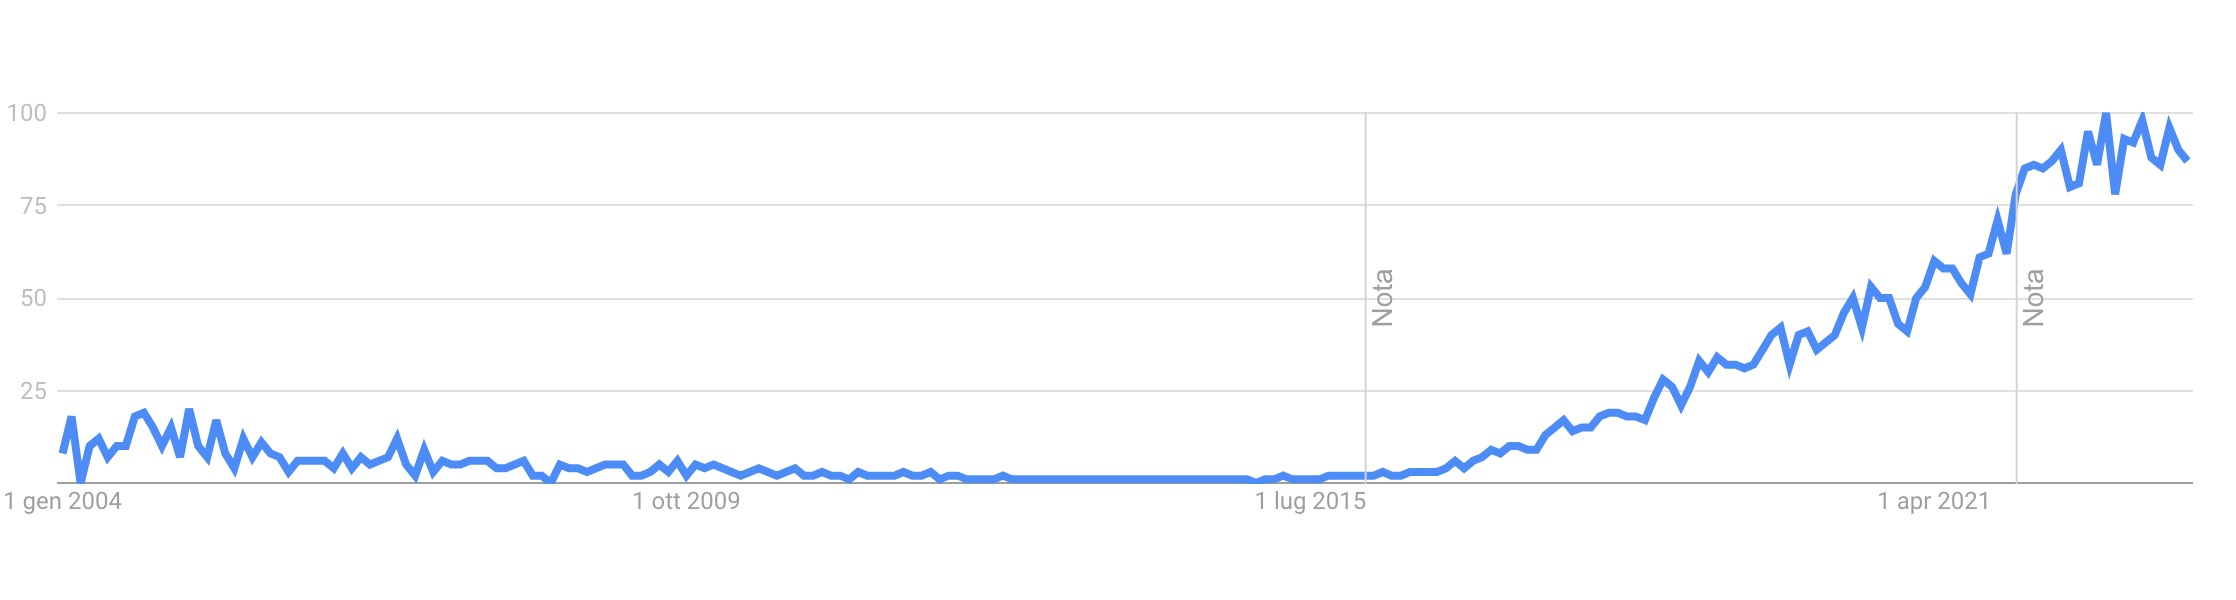
\includegraphics[width=12cm]{images/Trends_DT.jpg}
\caption[Grafico Google Trends ricerche sul Digital Twin]{Ricerche su \emph{Digital Twin} effettuate dal 2004 al 2023 su Google~\cite{Trends_DT}}\label{fig:trends}
\end{center}
\end{figure}

\subsection{Introduzione del Digital Twin}
Con l'avvento dell'Industria 4.0 il \emph{Digital Twin} è considerato di estrema importanza. I vari utilizzi del \emph{Digital Twin} in diversi settori includono la progettazione, pianificazione, ottimizzazione, manutenzione, sicurezza, presa di decisioni, accesso remoto e formazione. Può essere uno strumento prezioso per le aziende per aumentare la loro competitività, produttività ed efficienza~\cite{Campi_DT}.

\newpage

Il mercato globale del \emph{Digital Twin} è stato stimato a 3,1 miliardi di dollari nel 2020 e ci si aspetta che crescerà in modo esponenziale negli anni successivi (stimato intorno ai 137 miliardi per il 2030, figura \ref{fig:valutazione}).

\begin{figure}[h]
\begin{center}
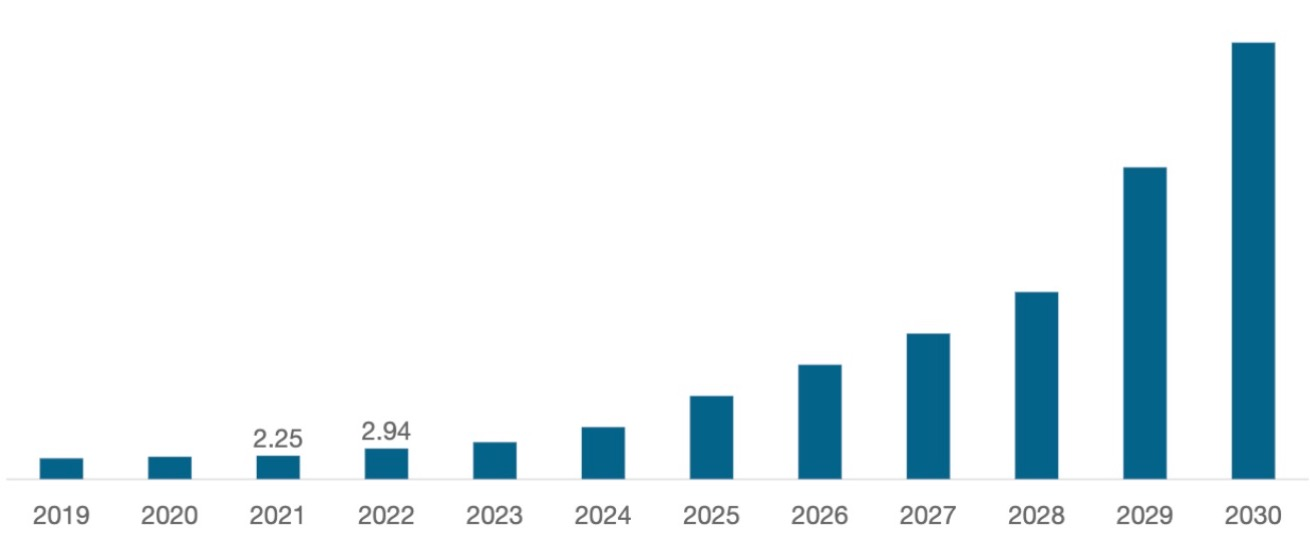
\includegraphics[width=12cm]{images/Market_DT.jpg}
\caption[Grafico valutazione Digital Twin]{Valutazione futura stimata sul \emph{Digital Twin}~\cite{Market_DT}}\label{fig:valutazione}
\end{center}
\end{figure}

La pandemia di COVID-19 ha cambiato il modo in cui vengono considerate la produzione e la manutenzione, accelerando l'adozione dei Digital Twin~\cite{Covid_DT}.

\subsection{Storia del Digital Twin}
Nonostante il \emph{Digital Twin} abbia guadagnato una grande popolarità negli ultimi anni, il concetto non è del tutto nuovo. Il suo concetto è emerso in relazione alla ”Gestione del Ciclo di Vita del Prodotto” nel 2002 presso l'Università del Michigan da Michael Grieves~\cite{Origin_DT}.

Il modello proposto ha tre componenti: prodotto reale, prodotto virtuale e un meccanismo di collegamento per il flusso di dati tra i due; il modello è stato poi chiamato ”Modello di Prodotti Specchiati”~\cite{Spazi_specchiati}. 

Un concetto simile, in cui i modelli software imitano la realtà a partire da informazioni provenienti dal mondo fisico, è stato immaginato da David Gelernter nel 1991 ed è stato chiamato ”Mondi Specchiati”~\cite{Mondi_specchiati}.

Entro il 2006, il nome del modello concettuale proposto da Grieves è stato cambiato da ”Modello di Prodotti Specchiati” a ”Modello di Riflessione delle Informazioni”~\cite{Origin_concept_DT, PLM_DT}.

Il nome \emph{Digital Twin} appare per la prima volta sotto forma di bozza in un articolo della NASA nel 2010~\cite{NASA2}. Nell'articolo della NASA, il \emph{Digital Twin} veniva anche definito ”Leader di Flotta Virtuale Digitale”. La NASA è stata la prima associazione a definire il \emph{Digital Twin}; è stato descritto come ”una simulazione integrata multi-fisica, multi-scala e probabilistica di un veicolo o sistema che utilizza i migliori modelli fisici disponibili, aggiornamenti dei sensori, storia della flotta, ecc., per riflettere la vita del suo gemello volante”~\cite{NASA}.

Anche se la prima menzione del \emph{Digital Twin} è nella roadmap del 2010, la NASA aveva utilizzato un concetto simile in passato per il programma Apollo, in cui venivano costruiti due veicoli spaziali identici per riflettersi a vicenda~\cite{Apollo}.

Successivamente la ”U.S. Air Force” ha seguito le orme della NASA ed ha utilizzato il \emph{Digital Twin} per la progettazione, la manutenzione e la previsione dei loro aerei~\cite{Air_force}. L'idea era quella di utilizzare il \emph{Digital Twin} per simulare le proprietà fisiche e meccaniche dell'aeromobile per prevedere qualsiasi affaticamento o crepa nella struttura.

Oltre al monitoraggio, il \emph{Digital Twin} è stato anche proposto per l'esplorazione spaziale sostenibile e per le future generazioni di veicoli aerospaziali~\cite{NASA}.

Dalla prima definizione mai pubblicata dalla NASA, diversi autori hanno descritto il \emph{Digital Twin} con termini propri e in base alla sua applicazione, definendolo come un modello virtuale~\cite{Fedelta, Airframe_DT, Def_DT, Def2_DT, Gerarchico, Complex_Aerostructures, DTH_DT}, una controparte digitale~\cite{Controparte1, Evolutivo}, un doppione ~\cite{IBM_DT}, un clone~\cite{Clone_DT} o una rappresentazione digitale~\cite{Rappresentazione1, Rappresentazione2, Rappresentazione3}.

Dopo che il \emph{Digital Twin} ha trovato un utilizzo in settori oltre la produzione, si è iniziato ad applicarlo anche ad entità biologiche complesse come gli esseri umani e gli alberi~\cite{Rappresentazione1, Alberi_DT}.

\newpage

Il \emph{Digital Twin} può svolgere compiti come:
\begin{itemize}
    \item Analisi approfondita del gemello fisico
    \item Progettazione e convalida di prodotti/processi nuovi o esistenti
    \item Simulazione delle condizioni di salute del gemello fisico
    \item Miglioramento della sicurezza e dell'affidabilità del gemello fisico
    \item Ottimizzazione di parti, prodotti, processi o linee di produzione
    \item Monitoraggio dello stato del gemello fisico durante tutta la sua vita
    \item Previsione delle prestazioni del gemello fisico
\end{itemize}

Le definizioni di \emph{Digital Twin} spesso trascurano la sua longevità; tuttavia, alcuni articoli considerano il \emph{Digital Twin} come un modello ”cradle-to-gravel ” (tradotto in italiano come ”dalla culla alla tomba”), significando che può essere utilizzato per l'intero ciclo di vita del prodotto, dal momento dell'ideazione fino alla sua eliminazione~\cite{Airframe_DT, Air_force, Culla, Culla2}.

Alcuni articoli~\cite{Economico} suggeriscono anche che il \emph{Digital Twin} può includere informazioni relative allo smaltimento del prodotto durante la fase di eliminazione. Inoltre, dopo che il prodotto è stato eliminato, il \emph{Digital Twin} può aiutare nella progettazione e produzione della generazione successiva~\cite{Riutilizzo}.

Il \emph{Digital Twin} è diverso dai modelli informatici (CAD/CAE) e dalla simulazione. Anche se molte organizzazioni lo utilizzano sinonimo a modello 3D, un modello 3D è solo una parte del \emph{Digital Twin}~\cite{Culla}.

Il \emph{Digital Twin} utilizza dati per riflettere il mondo reale in qualsiasi momento e quindi può essere utilizzato per osservare e comprendere le prestazioni del sistema e per la sua manutenzione predittiva~\cite{Sofisticazione}.

\newpage

\subsection{Vantaggi e caratteristiche del Digital Twin}
Dal momento in cui è stato introdotto per la prima volta, il \emph{Digital Twin} ha guadagnato sempre più popolarità, con sempre più ricercatori che hanno iniziato a concentrare la propria ricerca su questo argomento (figura \ref{fig:crescita_pubblicazioni}).

\begin{figure}[h]
\begin{center}
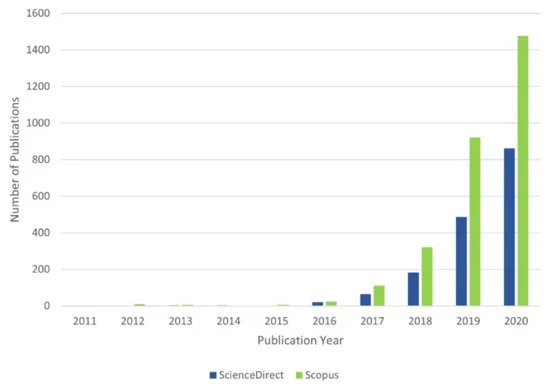
\includegraphics[width=12cm]{images/Pubblicazione_DT.jpg}
\caption[Grafico pubblicazione Digital Twin]{Trend di crescita sulla pubblicazioni del \emph{Digital Twin}~\cite{Researchgate}}\label{fig:crescita_pubblicazioni}
\end{center}
\end{figure}

La crescente popolarità del \emph{Digital Twin} è evidente dal fatto che è stato considerato come un argomento di tendenza nel campo tecnologico per tre anni consecutivi (2017-2019) da Gartner\cite{Gartner2017, Gartner2018, Gartner2019}, una tecnologia futura nel campo aerospaziale e della difesa da Lockheed Martin~\cite{Martin} e una delle tecnologie definitorie del prossimo decennio da Forbes~\cite{Forbes}

\newpage

\subsubsection{Vantaggi del Digital Twin}

La principale ragione per cui la tecnologia \emph{Digital Twin} è vista come la pietra angolare dell'Industria 4.0 risiede nella sua serie di vantaggi, che includono la riduzione di errori, incertezze, inefficienze e spese in qualsiasi sistema o processo. Inoltre, elimina tutti i compartimenti stagni nei processi o nelle organizzazioni che altrimenti operano in isolamento nelle strutture industriali più tradizionali. Alcuni dei vantaggi riportati per il \emph{Digital Twin} includono:
\begin{itemize}
    \item Velocità nella creazione e testing di un prototipo
    
    Poiché le simulazioni consentono l'analisi di numerosi scenari, i cicli di progettazione e analisi si accorciano, rendendo l'intero processo di lavoro con i prototipi più facile e veloce. Una volta implementato, il \emph{Digital Twin} può essere utilizzato in diverse fasi del processo di progettazione del prodotto, dalla concezione dell'idea del prodotto ai test~\cite{Testing_prototipo}. Poiché il \emph{Digital Twin} è collegato al suo gemello fisico per tutta la sua durata di testing, è possibile confrontare le prestazioni effettive e previste~\cite{Testing}.
    
    \item Economico
    
    Grazie al fatto che il \emph{Digital Twin} coinvolge principalmente risorse virtuali per la sua creazione, il costo complessivo di prototipazione diminuisce nel tempo.
    Nella prototipazione tradizionale, il ridisegno di un prodotto è dispendioso in termini di tempo e costi a causa dell'uso di materiali fisici e manodopera. Inoltre, un test che fallisce significa la fine di quel costoso prototipo. Utilizzando il \emph{Digital Twin}, i prodotti possono essere ricreati e sottoposti a test con alta probabilità di fallimento senza alcun costo aggiuntivo per i materiali. Quindi, assumendo che il costo sia uguale all'inizio, i costi fisici aumentano man mano che l'inflazione sale, ma i costi virtuali diminuiscono significativamente nel tempo~\cite{Economico}. Il \emph{Digital Twin} consente il testing dei prodotti in diverse situazioni operative, comprese quelle distruttive, senza costi aggiuntivi. Inoltre può ridurre i costi operativi e prolungare la vita utile delle attrezzature e degli asset una volta implementato.
    
    \item Previsione dei problemi
    
    Utilizzando il \emph{Digital Twin}, possiamo prevedere i problemi e gli errori per gli stati futuri del prodotto effettivo. Grazie ai dati in tempo reale che fluiscono tra l'oggetto fisico e il suo gemello digitale è possibile prevedere problemi durante le diverse fasi del ciclo di vita del prodotto. Questo è particolarmente vantaggioso per la gestione di strutture complesse che sono composte da materiali multipli come aerei, veicoli, attrezzature di fabbrica, ecc., poiché all'aumentare della complessità di un prodotto, diventa più difficile prevedere i guasti dei componenti con metodi convenzionali~\cite{Testing_prototipo}.
    
    \item Accessibilità
    
    Il dispositivo fisico può essere controllato e monitorato a distanza utilizzando il suo \emph{Digital Twin}. A differenza dei sistemi fisici, che sono limitati dalla loro posizione geografica, i sistemi virtuali (come il \emph{Digital Twin}) possono essere ampiamente condivisi e accessibili da remoto~\cite{Economico}. Il monitoraggio e il controllo a distanza di apparecchiature e sistemi diventano necessari in situazioni in cui l'accesso locale è limitato, come durante la pandemia di COVID-19 quando i governi hanno imposto blocchi e il lavoro a distanza o il contatto zero sono l'unica opzione praticabile~\cite{Covid_DT}.
    
    \item Sicurezza
    
    In settori come il settore petrolifero o minerario dove le condizioni di lavoro sono estremamente pericolose, la capacità del \emph{Digital Twin} di accedere da remoto al suo gemello fisico, così come la sua natura predittiva, può ridurre il rischio di incidenti e guasti pericolosi. Tuttavia, il vantaggio del \emph{Digital Twin} nell'accesso remoto non si limita alla prevenzione degli incidenti. Secondo un sondaggio di Gartner, quasi un terzo delle aziende ha utilizzato il \emph{Digital Twin} durante la pandemia per aumentare la sicurezza dei dipendenti e dei clienti attraverso il monitoraggio a distanza~\cite{Gartner_covid}.
    
    \item  Riduzione dei rifiuti

    Utilizzare il \emph{Digital Twin} per simulare e testare prototipi di prodotti in un ambiente virtuale riduce significativamente lo spreco di materiali. I prototipi possono essere sondati e controllati virtualmente, sotto una varietà di scenari di test diversi, per finalizzare il design del prodotto finale prima della produzione. Ciò non solo risparmia lo spreco di materiali, ma riduce anche i costi di sviluppo e il tempo di commercializzazione.

    \item Formazione del personale
    
    Il \emph{Digital Twin} può essere utilizzato per sviluppare programmi di formazione sulla sicurezza più efficienti e illustrativi rispetto a quelli tradizionali~\cite{Formazione}. Prima di operare in un ambiente ad alto rischio o su macchinari pericolosi, è possibile fornire agli operatori un addestramento attraverso l'utilizzo di un  \emph{Digital Twin} al fine di mitigare i rischi. L'istruzione relativa a vari processi o scenari li preparerà adeguatamente affinché possano affrontare in sicurezza situazioni simili di persona. Ad esempio, l'ambiente minerario è un ambiente ad alto rischio in cui i nuovi dipendenti possono essere addestrati utilizzando il \emph{Digital Twin} sull'utilizzo dei macchinari e su come affrontare scenari di emergenza~\cite{Mining}.
    
\end{itemize}

\newpage

\subsubsection{Caratteristiche del Digital Twin}

A seconda del tipo di \emph{Digital Twin}, può possedere proprietà distintive da altri, ma comunque tutti i \emph{Digital Twin} condividono alcune caratteristiche comuni:
\begin{itemize}
    \item Alta fedeltà
    
    Un \emph{Digital Twin} deve essere una copia quasi identica del suo gemello fisico in termini di aspetto, contenuti, funzionalità. Un modello digitale super realistico aiuta il \emph{Digital Twin} a imitare ogni aspetto del suo gemello fisico. I modelli informatici ad alta fedeltà sono considerati il suo fondamento. Questo livello di dettaglio consente agli strumenti di simulazione e previsione di essere più affidabili quando presentati con un insieme di azioni o scenari alternativi~\cite{Fedelta}.

    \item Dinamico

    Siccome il piano fisico è un sistema dinamico (a differenza del piano virtuale)  un \emph{Digital Twin} deve cambiare di conseguenza. Questo viene raggiunto attraverso la connessione continua e lo scambio di informazioni tra il mondo fisico e virtuale. Lo scambio di dati può riguardare dati dinamici, dati statici storici e dati statici descrittivi~\cite{Evolutivo}. L'obiettivo del \emph{Digital Twin} è di riflettere il comportamento del prodotto nel mondo digitale in qualunque momento~\cite{Culla}.

    \item Auto-evolutivo

    Il \emph{Digital Twin} si evolve insieme al suo gemello fisico durante l'intero ciclo di vita. Qualsiasi cambiamento sia nel \emph{Digital Twin} che nel prodotto è riflesso nell'altro, creando un ciclo di feedback continuo~\cite{Culla}. Un \emph{Digital Twin} è auto-adattante e auto-ottimizzante grazie ai dati raccolti dal gemello fisico in tempo reale, maturando quindi insieme al suo gemello fisico durante tutta la sua durata~\cite{Evolutivo}.

    \newpage

    \item Identificabile
    
    Ogni componente deve avere il proprio \emph{Digital Twin}. Durante diverse fasi del ciclo di vita del prodotto, i dati e le informazioni ad esso correlati si evolvono (inclusi modelli geometrici 3D, modelli di produzione, modelli di utilizzo, modelli funzionali, ecc ...). Grazie all'esistenza di tali modelli creati per il \emph{Digital Twin}, esso può essere identificato univocamente dal suo gemello fisico o viceversa per l'intera durata del suo ciclo di vita~\cite{Identificabile}.
    
    \item Gerarchico
    
    La natura gerarchica del \emph{Digital Twin} deriva dal fatto che i diversi componenti e parti che compongono il prodotto finale hanno il proprio modello \emph{Digital Twin} corrispondente, ad esempio il \emph{Digital Twin} di un aereo è composto da \emph{Digital Twin} di una specifica componente, \emph{Digital Twin} del sistema di controllo di volo, \emph{Digital Twin} del sistema di propulsione, ecc. Pertanto, un \emph{Digital Twin} può essere visto come una serie di sub-modelli integrati~\cite{Gerarchico}.
    
\end{itemize}

\subsection{Categorie del Digital Twin}
Il \emph{Digital Twin} può essere categorizzato in base alle sua applicazione~\cite{Economico}.

Le due principali applicazioni di un \emph{Digital Twin} sono la previsione e l'interrogazione~\cite{Economico}.
Un \emph{Digital Twin} predittivo, come suggerisce il nome, prevede il comportamento e le prestazioni future del suo corrispettivo fisico, mentre un \emph{Digital Twin} interrogativo è utilizzato per interrogare lo stato attuale o passato del suo corrispettivo fisico indipendentemente dalla sua posizione~\cite{Categoria}.

\newpage

I \emph{Digital Twin} possono anche essere suddivisi a seconda se l'attenzione dell'applicazione è sul prodotto, sul processo o sulle prestazioni~\cite{Categoria}:
\begin{itemize}
    \item \emph{Digital Twin} di Prodotto
    
    Viene utilizzato per la fase di gestione del prototipo poiché analizza il prodotto in diverse condizioni e si assicura che il successivo prodotto fisico si comporti come previsto. Questa fase può essere rapida in quanto il tempo di sviluppo complessivo viene ridotto e non è più necessario svilupparne molti.

    \item \emph{Digital Twin} di Produzione
    
    Viene utilizzato per convalidare i processi simulandoli e quindi analizzandoli anche prima della produzione effettiva. Ciò aiuta a sviluppare una metodologia di produzione efficiente in diverse condizioni. I dati provenienti dai \emph{Digital Twin} di Prodotto e Produzione possono essere utilizzati insieme per il monitoraggio e la manutenzione delle macchine.
    
    \item \emph{Digital Twin} di Prestazioni
    
    Viene utilizzato per i processi decisionali catturando, aggregando e analizzando i dati provenienti da prodotti e impianti intelligenti. Poiché il \emph{Digital Twin} di Prestazioni include le prestazioni sia del prodotto che della produzione, ottimizza le operazioni in base alla disponibilità delle risorse dell'impianto, creando un'opportunità per migliorare i \emph{Digital Twin} di Produzione e Prodotto attraverso un ciclo di feedback.
\end{itemize}

\newpage

\subsection{Gerarchia del Digital Twin}

Da una prospettiva gerarchica, i \emph{Digital Twin} possono essere suddivisi anche in tre diversi livelli (figura \ref{fig:gerarchia}), in base all'entità coinvolta nella produzione~\cite{Identificabile}:


\begin{figure}[h]
\begin{center}                      
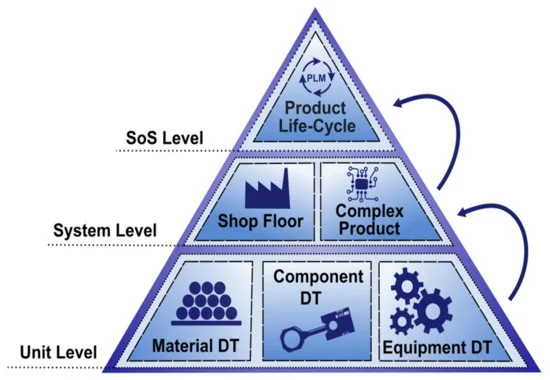
\includegraphics[width=10cm]{images/Gerarchia_DT.png}
\caption[Gerarchia del Digital Twin]{Gerarchia del Digital Twin}\label{fig:gerarchia}
\end{center}
\end{figure}

\begin{itemize}
    \item Livello di Unità (Unit level)
    
    È l'unità più piccola nella produzione e può essere un pezzo di attrezzatura, materiale o un fattore ambientale. Il \emph{Digital Twin} a livello di unità si basa sul modello geometrico, funzionale, comportamentale e operativo del corrispettivo fisico.

    \item Livello di Sistema (System level)
    
    È un'aggregazione di diversi \emph{Digital Twin} di livello unità in un sistema di produzione (come per esempio una fabbrica). L'interconnettività e la collaborazione tra molteplici \emph{Digital Twin} a livello di unità portano a un flusso più ampio di dati e a una migliore allocazione delle risorse. Un prodotto complesso, ad esempio un aereo, può essere considerato anche come \emph{Digital Twin} a livello di sistema.

    \item Livello di Sistema di Sistemi (SoS level)
    
    Un certo numero di \emph{Digital Twin} di livello di sistema è collegato insieme per formarne uno a livello di SoS, che aiuta la collaborazione tra diverse aziende o tra diversi dipartimenti di un'azienda (come la catena di approvvigionamento, il design, il servizio, la manutenzione). In altre parole, il \emph{Digital Twin} a livello di SoS integra diverse fasi del prodotto durante tutto il suo ciclo di vita.

\end{itemize}

\subsection{Livello di Maturità/Sofisticazione}

In base al livello di sofisticazione dei \emph{Digital Twin}, ovvero alla quantità e alla qualità dei dati ottenuti dal gemello fisico e dal suo ambiente, i \emph{Digital Twin} possono essere raggruppati in~\cite{DT_tipi}:

\begin{itemize}
    \item Digital Twin Parziale
    
    Contiene un piccolo numero di punti dati, ad esempio pressione, temperatura, umidità, ecc., utili per determinare la connettività e la funzionalità del \emph{Digital Twin}.

    \item Digital Twin Clone
    
    Contiene tutti i dati significativi e rilevanti provenienti dal prodotto/sistema che possono essere utilizzati per la creazione di prototipi e la categorizzazione delle fasi di sviluppo.

    \item Digital Twin Potenziato
    
    Utilizza i dati del gemello fisico insieme ai suoi dati storici e elabora i dati utili utilizzando algoritmi e analisi.
\end{itemize}

\newpage

I \emph{Digital Twin} possono diventare più sofisticati e precisi con l'accumulo di insiemi di dati più ampi nel corso del tempo di funzionamento. Il livello di maturità dei \emph{Digital Twin} non è limitato solo ai dati, ma comprende anche il livello di sofisticazione della rappresentazione/modello virtuale. Su questa base, i \emph{Digital Twin} sono suddivisi in quattro livelli~\cite{Sofisticazione}:

\begin{enumerate}
    \item Pre-Digital Twin
    
    Questo è il livello 1, in cui il \emph{Digital Twin} viene creato prima dell'asset fisico con lo scopo di prendere decisioni sul design del prototipo per ridurre qualsiasi rischio tecnico e risolvere anticipatamente i problemi utilizzando un modello di sistema generico.

    \item Digital Twin
    
    Il livello 2 incorpora i dati dell'asset fisico relativi alle sue prestazioni, salute e manutenzione. Il modello virtuale del sistema utilizza questi dati per assistere le decisioni ad alto livello nella progettazione e nello sviluppo dell'asset, insieme alla pianificazione della manutenzione. Il trasferimento dei dati a questo livello è bidirezionale.

    \item Digital Twin Adattativo
    
    Il livello 3 fornisce un'interfaccia utente adattiva tra l'asset fisico e il \emph{Digital Twin} e ha la capacità di imparare dalle preferenze e dalle priorità degli operatori umani utilizzando il machine learning supervisionato. Utilizzando questo \emph{Digital Twin}, è possibile la pianificazione e la presa di decisioni in tempo reale durante le operazioni.
    
    \item Digital Twin Intelligente
    
    Oltre alle caratteristiche del livello 3, il livello 4 ha la capacità di apprendimento automatico non supervisionato, rendendolo più autonomo rispetto al livello 3. Può riconoscere modelli nell'ambiente operativo e utilizzando questi dati insieme all'apprendimento rinforzato consente un'analisi più precisa ed efficiente del sistema.
    
\end{enumerate}

\section{Digital Thread}
Proprio come il concetto di \emph{Digital Twin}, il termine \emph{Digital Thread} nasce dall'industria aerospaziale, dove è nato come parte integrante di un processo di ingegneria dei sistemi avanzato, mirato alla gestione completa e digitale di tutte le fasi coinvolte. Inizialmente concepito per tracciare e coordinare le varie fasi di progettazione, produzione e distribuzione di un sistema complesso, il \emph{Digital Thread} si è rivelato fondamentale per la sincronizzazione di dati e informazioni lungo l'intero ciclo di vita del prodotto~\cite{Thread}.

Questo contesto pionieristico nell'industria aerospaziale ha visto il \emph{Digital Thread} come una rete intricata di molteplici dati, dai modelli CAD 3D alle strategie di produzione, dai dettagli logistici ai processi di assemblaggio~\cite{Thread2}.

Una delle sue caratteristiche principali è la capacità di fornire un flusso ininterrotto di informazioni, garantendole disponibili sempre disponibili a richiesta(figura \ref{fig:dth_example}). Rispetto al \emph{Digital Twin}, che funge da gemello virtuale in tempo reale di un oggetto fisico, il \emph{Digital Thread} agisce come una traccia storica, una sorta di cronologia digitale che registra e conserva ogni tappa e aspetto del ciclo di vita dell'oggetto fisico~\cite{Thread3}.

\begin{figure}[h]
\begin{center}
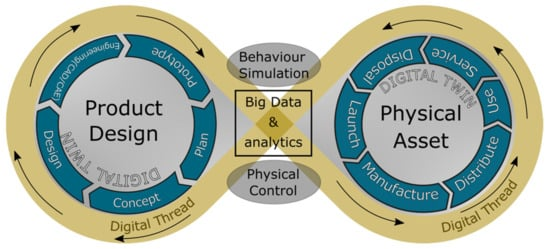
\includegraphics[width=12cm]{images/Example_DTH.jpg}
\caption[Esempio funzionamento Digital Thread]{Esempio funzionamento del \emph{Digital Thread}~\cite{Thread3}}\label{fig:dth_example}
\end{center}
\end{figure}

\newpage

Il \emph{Digital Thread} è uno dei fondamenti su cui si basa l'Industria 4.0. La convergenza di principi come l'\emph{Internet of Things} (IoT) – che consente ai dispositivi di raccogliere e scambiare dati –, la virtualizzazione, la decentralizzazione delle decisioni e la capacità di analizzare dati in tempo reale costituiscono esempi in cui viene altamente adottato l'intero concetto di \emph{Digital Thread}~\cite{Thread}.

\subsection{Vantaggi e Applicazioni}

L'implementazione del concetto del \emph{Digital Thread} ha dimostrato di portare molti benefici in diversi settori~\cite{Thread4}. La tracciabilità completa e digitale dei dati lungo l'intero ciclo di vita del prodotto ha un impatto significativo sull'efficienza operativa, sulla riduzione degli errori, sull'accelerazione dei tempi di produzione e sulla possibilità di offrire personalizzazione su larga scala~\cite{Thread}.

\begin{itemize}
    \item Miglioramento dell'Efficienza Operativa

    La capacità di tracciare ogni fase di un prodotto attraverso il \emph{Digital Thread} consente un controllo più rigoroso e una gestione ottimizzata dei processi. Ciò si traduce in una maggiore efficienza nella pianificazione e nell'esecuzione delle attività di produzione. Ad esempio, le aziende manifatturiere possono monitorare in tempo reale l'utilizzo delle risorse, identificando aree di sovrautilizzo o sottoutilizzo e apportando correzioni tempestive.

    \item Riduzione degli errori
    
    L'automazione del flusso di dati all'interno del \emph{Digital Thread} riduce significativamente il rischio di errori umani. Gli errori di trascrizione e di comunicazione vengono minimizzati poiché le informazioni vengono trasferite e condivise in modo accurato e coerente tra le diverse fasi del processo produttivo. Questo aspetto è particolarmente rilevante in settori ad alta precisione, come l'industria medica, dove anche un piccolo errore potrebbe avere conseguenze significative.

    \item Accelerazione dei tempi di produzione

    La collaborazione e l'accesso in tempo reale alle informazioni attraverso il \emph{Digital Thread} consentono una pianificazione più agile e una riduzione dei tempi di attesa. La condivisione istantanea di dati tra diversi reparti, fornitori e partner durante la produzione accelera il processo decisionale e riduce i ritardi.

    \item Personalizzazione su larga scala

    Uno dei vantaggi distintivi del \emph{Digital Thread} è la sua capacità di consentire la personalizzazione su larga scala. La tracciabilità digitale delle specifiche del prodotto e delle preferenze dei clienti consente la progettazione e la produzione di prodotti altamente personalizzati, senza sacrificare l'efficienza. Ad esempio, nell'industria dell'abbigliamento, le aziende possono creare capi su misura basati sui dati delle misurazioni dei clienti.
    
    \item Applicazioni in diversi settori
    
    Oltre all'industria aerospaziale, il concetto di \emph{Digital Thread} ha trovato applicazione in diverse altre industrie. Nel settore energetico, la gestione digitale delle risorse permette un monitoraggio continuo delle prestazioni e una manutenzione preventiva più efficace. Nell'industria alimentare, il \emph{Digital Thread} può tracciare l'intera filiera di produzione, aumentando la trasparenza e la sicurezza alimentare. Anche l'industria farmaceutica beneficia della tracciabilità digitale per garantire la conformità normativa e la sicurezza dei prodotti~\cite{Thread5}.
    
\end{itemize}

\newpage

\section{Digital shadow}

Nell'era contemporanea, il termine \emph{Digital Shadow} è emerso come un concetto che riflette l'impatto delle attività online sulla creazione di una sorta di ”ombra digitale”. Questo fenomeno rappresenta il riflesso virtuale delle azioni, delle interazioni e delle informazioni che lasciamo dietro di noi mentre interagiamo con il mondo digitale~\cite{Shadow}.

\subsection{Definizione}

Il \emph{Digital Shadow} rappresenta il complesso aggregato di dati, tracce digitali e informazioni personali che lasciamo involontariamente o volontariamente durante le nostre attività online. Questo spazia dalle ricerche su motori di ricerca, alle interazioni sui social media, agli acquisti online, alle conversazioni tramite e-mail e molto altro ancora. In altre parole, è la traccia virtuale che si forma attraverso le azioni nell'ambiente digitale. Questi dati vengono quindi utilizzati per profilare gli utenti, personalizzare le esperienze digitali e, in alcuni casi, per fini pubblicitari e di marketing~\cite{Shadow}.

\subsection{Vantaggi del \emph{Digital Shadow}}

Il \emph{Digital Shadow} ha portato a molteplici sviluppi positivi nella società moderna~\cite{Shadow}:

\begin{itemize}
    \item Personalizzazione delle esperienze
    
    Grazie al \emph{Digital Shadow}, le piattaforme possono offrire contenuti e servizi personalizzati, adattati alle preferenze individuali, migliorando così l'esperienza dell'utente.

    \item Avanzamenti tecnologici
    
    L'analisi dei dati del \emph{Digital Shadow} ha contribuito alla creazione di algoritmi di intelligenza artificiale e di apprendimento automatico, che guidano l'innovazione in vari settori, come la medicina, l'automazione industriale e altro ancora.

    \item Ricerca e innovazione
    
    Gli scienziati e i ricercatori possono utilizzare dati anonimi del \emph{Digital Shadow} per ottenere informazioni preziose sui modelli di comportamento e sulle tendenze sociali, facilitando così la ricerca e l'innovazione~\cite{Shadow2}.
\end{itemize}

\subsection{Preoccupazioni del \emph{Digital Shadow}}

Tuttavia, il concetto di \emph{Digital Shadow} suscita anche preoccupazioni significative, tra cui:

\begin{itemize}
    \item Privacy
    
    La raccolta e l'archiviazione dei dati del \emph{Digital Shadow} sollevano interrogativi sulla privacy individuale. La condivisione non autorizzata di informazioni personali può portare a violazioni della privacy e all'abuso delle informazioni sensibili.
    
    \item Rischio di utilizzo malevolo
    
    I dati del \emph{Digital Shadow} possono essere vulnerabili agli attacchi informatici e all'uso malevolo da parte di attori maligni, mettendo a rischio la sicurezza delle informazioni personali.
\end{itemize}

\subsection{Economia dei dati}

L'accumulo di dati nel \emph{Digital Shadow} ha innescato una rivoluzione nell'economia dei dati, trasformando radicalmente la dinamica aziendale e le strategie di mercato. Aziende di tutte le dimensioni stanno riconoscendo il valore inestimabile dei dati e il potenziale che essi offrono per comprendere meglio i consumatori e anticipare le tendenze di mercato~\cite{Shadow, Shadow_economy}.

Questo nuovo paradigma ha visto la nascita di un'industria incentrata sulla raccolta, l'elaborazione e lo sfruttamento dei dati del \emph{Digital Shadow}. Le aziende investono ingenti risorse per sviluppare algoritmi sofisticati e sistemi di analisi dei dati che possono estrapolare conoscenze preziose dai comportamenti e dalle preferenze degli utenti. Questi dati sono poi venduti a inserzionisti, aziende di marketing e altre organizzazioni che cercano di perfezionare le proprie strategie di promozione.

In questo contesto, i dati sono diventati una vera e propria moneta di scambio. Le aziende possono acquisire vantaggi competitivi attraverso l'accesso a dati accurati e approfonditi sulle abitudini dei consumatori. Tuttavia, questa crescente dipendenza dai dati ha sollevato interrogativi sulla trasparenza e sulla giustizia dell'acquisizione e della monetizzazione di tali informazioni~\cite{Shadow_economy, Sell_data}.

\subsection{Etica e regolamentazione del \emph{Digital Shadow}}

L'espansione incontrollata del \emph{Digital Shadow} ha innescato una serie di sfide etiche e legali che richiedono una risposta ponderata e regolamentazioni adeguate. La rapida raccolta e condivisione di dati sensibili ha sollevato interrogativi fondamentali sulla privacy individuale e sulla sovranità dei dati personali~\cite{Shadow_economy, Sell_data, Sell_data2}.

L'equilibrio tra l'innovazione tecnologica e la protezione della privacy è al centro del dibattito pubblico e politico~\cite{Sell_data2, Sell_data}. I governi stanno lavorando per introdurre normative che regolamentino la raccolta e l'uso dei dati personali, garantendo il consenso informato degli individui e stabilendo sanzioni per violazioni ed abusi~\cite{Law_Data}. Tuttavia, trovare il giusto equilibrio tra il potenziale beneficio dell'analisi dei dati e la salvaguardia della privacy è un compito complesso.
	\clearpage{\pagestyle{empty}\cleardoublepage}
\chapter{Tecnologie usate} 
Il secondo capitolo è dedicato alla presentazione delle diverse tecnologie impiegate, fornendo una base solida per la comprensione dell'ambiente tecnologico nel quale il progetto è stato realizzato.

\section{HTML}
”HyperText Markup Language”, comunemente abbreviato come HTML, è un linguaggio di markup utilizzato per creare e strutturare il contenuto delle pagine web. HTML è uno dei mattoni fondamentali su cui si basa il World Wide Web ed è ampiamente utilizzato per definire la struttura e l'organizzazione dei contenuti all'interno di una pagina web~\cite{Semantic_web, Core_web}.

HTML opera attraverso l'uso di elementi e tag. Ogni elemento è rappresentato da un tag che definisce il tipo di contenuto che conterrà. Ad esempio, il tag <h1> indica un'intestazione di primo livello, mentre il tag <p> rappresenta un paragrafo di testo. La corretta scelta dei tag è essenziale per garantire la semantica e l'accessibilità del contenuto~\cite{Core_web}.

Gli elementi HTML possono essere nidificati all'interno di altri elementi, creando una struttura gerarchica. Questa struttura permette di organizzare i contenuti in modo logico e ordinato. Ad esempio, è possibile includere un paragrafo all'interno di un'area specifica di una pagina, come un'intestazione o un piè di pagina.

HTML è stato sviluppato con l'obiettivo di fornire una struttura semantica per il contenuto web. L'utilizzo corretto dei tag non solo aiuta i motori di ricerca a comprendere meglio il contenuto, ma è anche fondamentale per migliorare l'accessibilità del sito. L'aggiunta di attributi come alt per le immagini o l'utilizzo di tag di intestazione in modo appropriato può rendere il contenuto accessibile anche a persone con disabilità.

In conclusione, l'HTML rappresenta il fondamento su cui si basa gran parte del World Wide Web. La sua capacità di strutturare e organizzare il contenuto in modo logico e significativo è essenziale per la creazione di pagine web funzionali e accessibili~\cite{Semantic_web}.

\section{CSS}
I ”Cascading Style Sheets”, comunemente noti come CSS, sono un linguaggio utilizzato per definire l'aspetto e la presentazione dei documenti HTML. CSS separa la struttura e il contenuto di una pagina web dalla sua formattazione visiva, consentendo agli sviluppatori di creare layout accattivanti e coerenti su diverse pagine~\cite{Core_web}.

Una delle caratteristiche principali di CSS è la sua capacità di separare i contenuti dalla presentazione. Questo significa che il contenuto di una pagina web, definito tramite HTML, può essere stilizzato e formattato in modo indipendente tramite il CSS. Questa separazione favorisce la manutenibilità, in quanto le modifiche visive possono essere apportate senza dover riscrivere il contenuto stesso~\cite{Core_web, ALL_WEB}.

CSS utilizza il concetto di ”cascata” per applicare stili ai vari elementi della pagina. Quando più regole vanno in conflitto per lo stesso elemento, viene utilizzata la selettività per determinare quale regola avrà la priorità. Inoltre, gli stili possono essere ereditati dagli elementi genitori agli elementi figli, semplificando l'applicazione coerente di stili a diverse parti del documento~\cite{ALL_WEB}.

CSS è essenziale per creare layout responsivi, che si adattano automaticamente alle diverse dimensioni dello schermo utilizzando tecniche come le ”media query” che permettono di creare layout diversi in base alla dimensione dello schermo.

CSS offre la possibilità di creare animazioni e transizioni. Gli sviluppatori possono definire cambiamenti di stile gradualmente nel tempo, creando effetti di transizione fluidi e dinamici. Inoltre, le trasformazioni CSS consentono di modificare la posizione, la rotazione e la scala degli elementi, aggiungendo un tocco di dinamicità alla presentazione.

In conclusione, i Cascading Style Sheets sono uno strumento essenziale per definire l'aspetto visivo delle pagine web. La loro capacità di separare i contenuti dalla presentazione, insieme alla flessibilità nella definizione di layout, colori, tipografia e animazioni, ha contribuito a creare esperienze web coinvolgenti e coerenti. CSS è un pilastro fondamentale nello sviluppo di pagine web moderne e accessibili.



\section{Javascript}
Javascript è un linguaggio di programmazione ampiamente utilizzato per aggiungere interattività e dinamicità alle pagine web. È comunemente usato per gestire eventi, manipolare il contenuto della pagina in risposta all'input dell'utente e comunicare con i server per ottenere o inviare dati in background~\cite{Javascript, ALL_WEB}.

Uno dei punti di forza di Javascript è la sua capacità di gestire gli eventi generati dagli utenti, come clic del mouse, pressioni di tasti e scorrimento. Questa interazione permette di creare esperienze web fluide e coinvolgenti, migliorando l'usabilità e l'interazione con i visitatori del sito~\cite{Javascript}.

Il ”Document Object Model” (DOM) rappresenta la struttura gerarchica degli elementi HTML all'interno di una pagina. Javascript consente di manipolare il DOM, aggiungendo, rimuovendo o modificando elementi in tempo reale. Questa manipolazione dinamica permette di creare contenuti interattivi senza dover ricaricare l'intera pagina~\cite{ALL_WEB, Javascript}.

\subsection{AJAX}
Javascript è spesso utilizzato per effettuare richieste asincrone al server attraverso la tecnica conosciuta come ”Asynchronous Javascript and XML”(AJAX). Questa tecnica consente di aggiornare parti specifiche di una pagina senza dover ricaricare l'intera pagina, migliorando la velocità e l'efficienza dell'esperienza utente~\cite{ALL_WEB}.

\subsection{Framework e librerie}
Nel corso degli anni, sono stati sviluppati numerosi framework e librerie Javascript per semplificare e accelerare lo sviluppo web. Alcuni esempi includono \href{https://angular.io/}{Angular}, \href{https://react.dev/}{React.js} e \href{https://vuejs.org/}{Vue.js}. Queste librerie offrono strumenti per creare interfacce utente complesse e gestire lo stato dell'applicazione in maniera più efficiente.

\section{Leaflet}
Leaflet è una libreria Javascript open-source utilizzata per creare mappe interattive e integrate nelle applicazioni web~\cite{Leaflet}. È progettata per essere leggera, flessibile e facile da utilizzare, consentendo agli sviluppatori di aggiungere funzionalità di mappatura ai loro progetti senza un carico eccessivo.

\newpage

\subsection{Caratteristiche principali}
Leaflet offre numerose funzionalità che la rendono una scelta popolare per la creazione di mappe interattive:

\begin{itemize}
    \item Mappatura Interattiva
    
    Permette agli sviluppatori di creare mappe interattive con zoom, panoramica e altri tipi di controlli.

    \item Layer Multipli
    
    Consente di sovrapporre diversi tipi di dati sulla mappa, come marcatori, linee e poligoni.

    \item Supporto per Dati Geospaziali
    
    Può visualizzare dati geospaziali provenienti da diverse fonti (come GeoJSON~\cite{GeoJSON}, GPX~\cite{GPX} e KML~\cite{KML}).
    
\end{itemize}

\section{Vue.js}
Vue.js è un framework Javascript open-source che facilita la creazione di interfacce utente interattive e complesse. Si basa sul modello ”Model-View-ViewModel” (MVVM) e offre strumenti per la gestione dello stato dell'applicazione e la creazione di componenti riutilizzabili~\cite{Vue}.

Una delle caratteristiche chiave di Vue.js è la sua architettura orientata ai componenti. L'interfaccia utente viene scomposta in componenti autonomi, ciascuno dei quali può avere il proprio stato, logica e template. Questa struttura favorisce la modularità e la riusabilità del codice.

Vue.js offre un sistema di two-way data binding, che collega automaticamente i dati del modello (lo stato dell'applicazione) alla vista (l'interfaccia utente). Ciò significa che le modifiche nello stato vengono riflesse automaticamente nell'interfaccia utente e viceversa, semplificando la sincronizzazione tra dati e visualizzazione.

Vue.js semplifica la gestione degli eventi, consentendo di associare metodi definiti nell'istanza Vue.js a eventi specifici. Questo permette di catturare l'interazione dell'utente e reagire ad essa in modo appropriato, aggiornando lo stato o eseguendo azioni specifiche.

Vue.js supporta anche il rendering lato server (SSR), che consente di generare il markup HTML direttamente sul server prima che venga consegnato al browser. Questa tecnica può migliorare le prestazioni iniziali e l'indicizzazione del contenuto da parte dei motori di ricerca.

Vue.js è sostenuto da una vivace comunità di sviluppatori che contribuiscono con componenti, plugin e risorse educative. La cura del framework e la sua attiva evoluzione lo hanno reso una scelta popolare per lo sviluppo di applicazioni web moderne.


\subsection{Libreria VueLeaflet}
\href{https://github.com/vue-leaflet/vue-leaflet}{VueLeaflet} è una libreria open-source che integra la potenza di Leaflet con il framework Javascript Vue.js. Questa libreria consente agli sviluppatori di creare mappe interattive in applicazioni Vue.js in modo semplice e integrato.

\subsubsection{Funzionalità Chiave}
VueLeaflet offre diverse caratteristiche che semplificano l'integrazione di mappe in applicazioni Vue.js:

\begin{itemize}
    \item Componenti Vue.js
    
    Le mappe e gli elementi di Leaflet possono essere trattati come componenti Vue.js, consentendo l'utilizzo di dati reattivi.

    \item Integrazione Diretta
    
    La libreria si integra facilmente con i componenti Vue.js esistenti.

    \item Personalizzazione
    
    Può essere personalizzata attraverso le opzioni di configurazione, consentendo di controllare l'aspetto e il comportamento delle mappe.

    \item Eventi Vue.js
    
    Gli eventi di Leaflet possono essere mappati agli eventi Vue.js, consentendo l'interazione tra le mappe e altri componenti.
\end{itemize}


\section{NPM}
Il Node Package Manager, abbreviato come NPM, è un gestore di pacchetti per l'ecosistema Javascript~\cite{NPM}. È utilizzato principalmente in ambienti di sviluppo Node.js per la gestione e la distribuzione di librerie, moduli e risorse necessarie per la creazione di applicazioni web e server-side~\cite{Nodejs}.

NPM consente agli sviluppatori di definire e gestire facilmente le dipendenze dei progetti Javascript. Attraverso un file proprietario è possibile elencare tutte le librerie esterne necessarie per il progetto, specificandone le versioni compatibili. Questo assicura che tutti i membri del team utilizzino le stesse versioni delle librerie e semplifica la collaborazione.

Oltre alla gestione delle dipendenze, NPM consente agli sviluppatori di definire comandi personalizzati. Questi comandi, chiamati ”NPM scripts”, possono essere utilizzati per eseguire attività come il build, il testing e l'avvio dell'applicazione. Questa funzionalità semplifica l'automazione di diverse operazioni di sviluppo.

Grazie a NPM, gli sviluppatori possono anche pubblicare i loro pacchetti e librerie per essere utilizzati da altri. Questa condivisione promuove la collaborazione e la condivisione di risorse all'interno della comunità di sviluppatori.

NPM supporta anche la gestione di progetti monorepo, in cui più pacchetti sono contenuti all'interno di un unico repository. Questo approccio semplifica la condivisione di codice tra diverse parti di un'applicazione e consente di gestire meglio le dipendenze condivise.

NPM offre strumenti per la gestione della sicurezza delle dipendenze, permettendo agli sviluppatori di rilevare vulnerabilità note nei pacchetti installati e di ricevere avvisi e aggiornamenti sulle possibili minacce.

\section{PHP}
PHP è un linguaggio di programmazione server-side ampiamente utilizzato per lo sviluppo di applicazioni web dinamiche e interattive. Una delle caratteristiche distintive di PHP è la sua capacità di generare HTML dinamicamente, consentendo la creazione di pagine web che possono interagire con gli utenti e con i dati nel server~\cite{ALL_WEB, PHP}.

Una delle principali ragioni per cui PHP è popolare nello sviluppo web è la sua integrazione nativa nel markup HTML. All'interno di un file HTML, è possibile includere del codice PHP, consentendo di mescolare codice PHP e HTML all'interno della stessa pagina.

PHP viene eseguito lato server, il che significa che il codice PHP è eseguito sul server web prima di inviare il risultato al browser dell'utente. Questo consente di elaborare dati e generare contenuti dinamici prima che raggiungano l'utente, migliorando la velocità e l'efficienza del sito.

PHP offre strumenti potenti per la manipolazione dei dati. È possibile interagire con database, leggere e scrivere file, elaborare dati di form e gestire cookie e sessioni. Queste capacità rendono PHP un'opzione versatile per la creazione di applicazioni web che richiedono l'interazione con il database e la gestione degli utenti.

Sebbene PHP abbia iniziato come un linguaggio adatto a script semplici, con il passare degli anni è stato potenziato per gestire applicazioni web complesse. Tuttavia, la sua architettura tradizionale basata su richieste può portare a sfide di performance in applicazioni ad alto traffico. È importante considerare strategie di caching e ottimizzazione quando si sviluppano applicazioni PHP scalabili.

La sicurezza è un aspetto cruciale nello sviluppo PHP. A causa delle sue radici come linguaggio per il web, PHP è spesso soggetto a vulnerabilità come le iniezioni SQL~\cite{Sql_Injection, SQL_Injection2} o le vulnerabilità di cross-site scripting (XSS)~\cite{XSS}. È essenziale adottare buone pratiche di sicurezza, come la validazione dei dati di input e l'uso di parametri preparati nelle query al database.

PHP continua a evolversi grazie agli sforzi della community e alle versioni successive del linguaggio. Nuove funzionalità e miglioramenti sono introdotti regolarmente, mantenendo PHP rilevante e adatto allo sviluppo di applicazioni web moderne.
\section{API}
Un'\emph{Application Programming Interface} (API) è un insieme di definizioni e protocolli che consentono a diversi software di comunicare tra loro. Le API fungono da intermediari, consentendo a diverse applicazioni di scambiare dati e funzionalità in modo standardizzato e strutturato~\cite{API}.

Le API consentono a diverse applicazioni o servizi di interagire tra loro, scambiando dati, richieste e risposte. Una API può fornire accesso a funzionalità specifiche dell'applicazione senza dover condividere l'intero codice sorgente. Questo favorisce la modularità e la collaborazione tra diversi team di sviluppo.

\subsection{Tipi di API}
Le API generalmente possono essere classificate in 3 diverse categorie:
\begin{itemize}
    \item Web API
    
    Consentono alle applicazioni di interagire tramite il protocollo HTTP, come RESTful APIs~\cite{API_WEB}.

    \item Librerie di API
    
    Forniscono un insieme di funzioni e metodi che le applicazioni possono utilizzare come parte di una libreria o framework~\cite{API_library}.

    \item API di Sistema Operativo
    
    Consentono alle applicazioni di interagire con il sistema operativo sottostante per accedere a risorse come file, processi e altro~\cite{API_SO}.

\end{itemize}

\subsection{RESTful APIs}
Le \emph{Representational State Transfer} (RESTful) APIs sono un tipo comune di API Web che seguono i principi dell'architettura REST. Utilizzano i metodi HTTP (GET, POST, PUT, DELETE) per gestire le operazioni CRUD (Create, Read, Update, Delete) sui dati. Le RESTful APIs utilizzano URL e risposte in formato JSON o XML~\cite{REST, REST2, ALL_WEB}.

\subsection{Uso delle API}
Le API sono utilizzate in una varietà di scenari~\cite{API_usage}:
\begin{itemize}
    \item Integrazione
    
    Le applicazioni possono integrare funzionalità di terze parti, come le API di pagamento o le API di social media.

    \item Automazione
    
    Le API consentono l'automazione di processi attraverso l'interazione programmata con servizi esterni.

    \item Accesso ai dati
    
    Le API possono fornire accesso a dati esterni, come le API che restituiscono dati meteorologici o finanziari.

    \item Sviluppo di plugin
    
    Le API consentono a sviluppatori esterni di creare plugin o estensioni per applicazioni esistenti.
\end{itemize}


\subsection{Documentazione}
Una buona documentazione delle API è essenziale per consentire agli sviluppatori di utilizzarle correttamente. La documentazione dovrebbe includere informazioni dettagliate su come autenticarsi, quali endpoint utilizzare e quali parametri passare.

\subsection{Evoluzione delle API}
Le API possono evolvere nel tempo, il che può causare sfide di retrocompatibilità. Esse dovrebbero consentire agli sviluppatori di continuare a utilizzare versioni precedenti fino a quando sono pronti per aggiornarsi alla versione successiva.

\section{JSON}
JSON, acronimo di Javascript Object Notation, è un formato leggero di scambio di dati utilizzato per rappresentare oggetti e dati strutturati in modo semplice e leggibile. Sebbene sia strettamente associato a Javascript (attraverso l'utilizzo di AJAX), JSON è diventato uno standard universale utilizzato in una varietà di linguaggi di programmazione~\cite{JSON, JSON_XML, GeoJSON}.

JSON utilizza una sintassi chiara e minimale. Gli oggetti vengono rappresentati come coppie chiave-valore, mentre gli array sono elenchi ordinati di valori. Questa struttura è facilmente leggibile dagli esseri umani e di facile elaborazione per le macchine.

Esso è diventato lo standard per lo scambio di dati tra client e server nelle applicazioni web. Molte API restituiscono dati in formato JSON, consentendo alle applicazioni di comunicare in modo efficiente attraverso il web.

JSON supporta la struttura gerarchica e la nidificazione. Gli oggetti possono contenere altri oggetti o array, consentendo la rappresentazione di dati complessi. Questa struttura rende JSON adatto per rappresentare dati strutturati e organizzati in modo logico.

JSON deve seguire una sintassi specifica per essere valido. Gli errori di formattazione possono impedire il corretto parsing dei dati. Fortunatamente, molti linguaggi di programmazione offrono strumenti incorporati per il parsing e la generazione di JSON corretti.

JSON negli  anni è diventato uno standard ubiquo per la rappresentazione di dati strutturati. La sua semplicità, leggibilità, compattezza e adozione generalizzata lo rendono un formato ideale per lo scambio di dati tra applicazioni, sia nell'ambiente web che in altri contesti di sviluppo. La sua capacità di rappresentare oggetti complessi in modo chiaro e strutturato ha contribuito a semplificare la comunicazione e l'interscambio di informazioni tra sistemi software.

\section{XML}
L'~\emph{eXtensible Markup Language}, comunemente noto come XML, è un linguaggio di markup utilizzato per rappresentare dati strutturati in un formato leggibile sia per gli esseri umani che per le macchine. XML è progettato per consentire la creazione di tag personalizzati e definire la struttura gerarchica dei dati.

XML è organizzato gerarchicamente attraverso l'utilizzo di tag e elementi. Ogni elemento è racchiuso tra tag di apertura e chiusura. Gli elementi possono essere nidificati per creare una struttura a albero che riflette la relazione tra i dati.

Una delle caratteristiche chiave di XML è la sua versatilità. Gli sviluppatori possono definire i propri tag personalizzati e strutturare i dati in base alle esigenze specifiche dell'applicazione. Questa flessibilità consente di rappresentare una vasta gamma di tipi di dati e informazioni.

XML viene utilizzato in una varietà di contesti, tra cui configurazioni di software, scambio di dati tra applicazioni e rappresentazione di informazioni complesse. Ad esempio, i file di configurazione di molti programmi sono spesso scritti in XML per consentire la personalizzazione delle impostazioni~\cite{XML, JSON_XML}.

XML è spesso utilizzato insieme ad altre tecnologie come XSLT (eXtensible Stylesheet Language Transformations) per trasformare i dati XML in formati diversi~\cite{XLST}, e XPath per navigare e selezionare parti specifiche dei documenti XML~\cite{XPATH}.

\subsection{JSON contro XML}
Negli ultimi anni, JSON (Javascript Object Notation) ha guadagnato popolarità come formato per lo scambio di dati. JSON è noto per essere più compatto e facilmente leggibile dalle macchine rispetto a XML. Tuttavia, XML è ancora ampiamente utilizzato in scenari che richiedono una struttura più flessibile o l'uso di metadati più avanzati~\cite{JSON_XML}.

\section{SQL}
\emph{Structured Query Language} (SQL) è un linguaggio di programmazione utilizzato per gestire e manipolare database relazionali. SQL offre un insieme di comandi standardizzati che consentono di creare, modificare, interrogare e gestire dati in tabelle strutturate.

SQL è basato su una struttura di dati relazionali, in cui i dati sono organizzati in tabelle con righe e colonne. Le tabelle rappresentano entità e relazioni nel mondo reale, e SQL offre un modo per definire schemi, inserire dati, modificarli e recuperarli~\cite{ALL_WEB}.

\subsection{Normalizzazione dei dati}
La normalizzazione è una pratica di progettazione dei database che mira a ridurre la duplicazione dei dati e migliorare l'efficienza delle interrogazioni. Attraverso la normalizzazione, i dati sono suddivisi in tabelle separate per minimizzare la ridondanza e massimizzare l'integrità~\cite{Normalizzazione}.

L'ottimizzazione delle interrogazioni è un aspetto critico nella gestione dei database. Gli sviluppatori devono scrivere query efficienti, utilizzare indici adeguati e considerare le prestazioni durante la progettazione del database per garantire tempi di risposta rapidi.

La sicurezza dei dati è fondamentale in SQL. È importante utilizzare pratiche di sicurezza come preparare i parametri prima di passarglieli per prevenire le iniezioni SQL, limitare i privilegi di accesso e crittografare i dati sensibili.

\section{XAMPP}
XAMPP è un pacchetto di software gratuito e open-source che fornisce un ambiente di sviluppo completo per la creazione di applicazioni web localmente. L'acronimo XAMPP sta per ”Cross-Platform (X), Apache (A), MySQL (M), PHP (P), Perl (P)”, che sono i componenti principali che costituiscono il pacchetto~\cite{XAMPP}.

\subsection{Componenti di XAMPP}
XAMPP include diversi componenti chiave:

\begin{itemize}
    \item Apache
    
    Un server web open-source che permette di ospitare e distribuire siti web.

    \item MySQL
    
    Un sistema di gestione di database relazionali (DBMS) per l'archiviazione e la gestione dei dati.

    \item PHP
    
    Un linguaggio di scripting server-side ampiamente utilizzato per creare applicazioni web dinamiche.

    \item Perl
    
    Un linguaggio di programmazione utilizzato per l'automazione di azioni e la creazione di script.

    \item phpMyAdmin
    
    Un'applicazione web che semplifica la gestione dei database MySQL attraverso un'interfaccia grafica.
\end{itemize}

XAMPP consente agli sviluppatori di creare un ambiente di sviluppo web sul proprio computer, eliminando la necessità di un server web esterno. Questo ambiente locale è ideale per lo sviluppo, il test e la risoluzione dei problemi delle applicazioni web prima di renderle pubbliche~\cite{XAMPP, ALL_WEB}.

\subsection{Configurazione e gestione}
XAMPP semplifica la configurazione dei componenti del server, consentendo agli sviluppatori di avviare e arrestare Apache, MySQL e altri servizi con poche azioni. Anche la configurazione delle impostazioni di PHP e MySQL può essere gestita attraverso l'interfaccia grafica di XAMPP.

\subsection{Testing e sicurezza}
XAMPP è particolarmente utile per sviluppatori e per i team che lavorano su progetti web. Fornisce un ambiente controllato in cui è possibile testare applicazioni, verificare la compatibilità tra componenti e risolvere i problemi senza dover pubblicare costantemente su un server esterno.

Tuttavia, è importante tenere presente che XAMPP è pensato principalmente per l'uso in ambienti di sviluppo e test. Non è ottimizzato per la sicurezza in un ambiente di produzione e non è raccomandato eseguirlo su un server accessibile pubblicamente.

\section{MySQL}
MySQL è un sistema di gestione di database relazionali (DBMS) open-source ampiamente utilizzato per archiviare, gestire e recuperare dati. È una scelta popolare sia per applicazioni web che per applicazioni di business grazie alla sua affidabilità, scalabilità e funzionalità avanzate~\cite{XAMPP, ALL_WEB}.

\subsection{Struttura dei Dati Relazionali}
MySQL si basa su una struttura dati relazionali in cui i dati sono organizzati in tabelle con righe e colonne. Questo approccio permette di rappresentare e gestire dati complessi in modo strutturato, permettendo la creazione di relazioni tra tabelle.

MySQL offre molte caratteristiche importanti:
\begin{itemize}
    \item Affidabilità
    
    È noto per la sua stabilità e robustezza, rendendolo adatto a scenari di produzione critici.

    \item Performance
    
    MySQL è ottimizzato per ottenere alte prestazioni in situazioni ad alto carico.

    \item Scalabilità
    
    È possibile scalare MySQL attraverso la distribuzione di server multipli o l'uso di tecnologie di replica.

    \item Gestione dei dati
    
    Supporta varie operazioni di gestione dei dati come l'indicizzazione, le transazioni e le viste.

    \item Sicurezza
    
    Offre meccanismi di autenticazione e autorizzazione per proteggere i dati.
\end{itemize}

\subsection{Uso nelle Applicazioni Web}
MySQL è ampiamente utilizzato nelle applicazioni web per la gestione di dati di back-end. Molti framework e CMS (Content Management System) supportano MySQL come database predefinito.

\section{Apache HTTP Server}
\emph{Apache HTTP Server}, spesso indicato semplicemente come Apache, è un server web open-source ampiamente utilizzato per ospitare siti web e distribuire contenuti su Internet~\cite{XAMPP, APACHE}.

Apache offre numerose funzionalità che lo rendono una scelta affidabile per l'hosting di siti web~\cite{APACHE}:
\begin{itemize}
    \item Server Web

    Apache è progettato per servire sia pagine web statiche che dinamiche agli utenti attraverso il protocollo HTTP.

    \item Virtual Hosting
    
    Supporta la creazione di più siti web su un singolo server attraverso l'utilizzo di virtual hosts.

    \item Modularità
    
    Apache è altamente modulare, consentendo agli amministratori di attivare solo i moduli necessari per soddisfare le esigenze specifiche del server.

    \item Autenticazione e Autorizzazione
    
    Apache offre meccanismi per controllare l'accesso alle risorse web attraverso l'autenticazione e l'autorizzazione.

    \item Reverse Proxy
    
    Può essere configurato come reverse proxy per indirizzare le richieste in arrivo a server back-end.
\end{itemize}

La configurazione di Apache avviene attraverso file di configurazione, tipicamente denominati \emph{httpd.conf} o \emph{apache2.conf}. Questi file contengono direttive che definiscono il comportamento del server, come i percorsi delle risorse, le opzioni di sicurezza e le regole di rewriting~\cite{APACHE, XAMPP}.


\section{Git}
Git è un sistema di controllo delle versioni distribuito open-source che consente agli sviluppatori di tenere traccia delle modifiche apportate al codice sorgente di un progetto nel tempo~\cite{GIT, GIT2}.

È ampiamente utilizzato per il coordinamento del lavoro di squadra, la gestione delle modifiche e il mantenimento della storia delle versioni di un progetto software.

Git si basa su alcuni concetti fondamentali:

\begin{itemize}
    \item Repository
    
    È la collezione di tutti i file e la loro storia associata. I repository possono essere locali o remoti.

    \item Commit
    
    Rappresenta una singola versione del codice sorgente all'interno del repository. I commit tengono traccia delle modifiche apportate.
    
    \item Branch
    
    È un ramo separato all'interno di un repository che può contenere modifiche indipendenti. È utilizzato per sviluppare nuove funzionalità senza influenzare il ramo principale.

    \item Merge
    
    È il processo di combinazione delle modifiche apportate in un ramo con un altro. Viene spesso utilizzato per integrare le modifiche di un ramo di sviluppo in un ramo principale.

    \item Push e Pull
    
    Caricare i commit nel repository remoto e sincronizzarsi con le modifiche altrui.

\end{itemize}

\subsection{Vantaggi di Git}
Git offre diversi vantaggi~\cite{GIT2}:

\begin{itemize}
    \item Storia delle versioni
    
    Mantiene un registro storico dettagliato delle modifiche, consentendo di risalire al momento e al motivo di ciascuna modifica.

    \item Collaborazione semplificata
    
    Consente a più sviluppatori di lavorare contemporaneamente su diverse parti del progetto.

    \item Gestione dei conflitti
    
    Fornisce strumenti per gestire conflitti che possono sorgere quando più persone modificano lo stesso file contemporaneamente.

    \item Sicurezza dei Dati
    
    Il codice sorgente è distribuito in diverse copie, riducendo il rischio di perdita di dati.
\end{itemize}


\subsection{Piattaforme di Hosting}
Esistono diverse piattaforme di hosting, come \href{https://github.com/}{GitHub}, \href{https://about.gitlab.com/}{GitLab} e \href{https://bitbucket.org/product}{Bitbucket}, che forniscono servizi per ospitare repository Git in modo che siano accessibili a team di sviluppo o al pubblico.


	\clearpage{\pagestyle{empty}\cleardoublepage}
\chapter{Visualizzazione dei Percorsi Escursionistici}
%%%%%%%%%%%%%%%%%%%%%%%%%%%%%%%%%%%%%%%%%imposta l'intestazione di pagina

% Questo capitolo avrà lo scopo di introdurre l'applicazione web sviluppata, mettendo in evidenza i principali obiettivi, le sfide affrontate e le soluzioni implementate. Inoltre verrà fornita una panoramica delle schermate chiave dell'applicazione.

Questo capitolo avrà lo scopo di introdurre l'applicazione web sviluppata, mettendo in evidenza sia l'ambiente di lavoro (mostrando le varie regole per mantenere un codice pulito e leggibile) sia i principali obiettivi, le sfide affrontate e le soluzioni implementate. Inoltre verrà fornita una panoramica delle schermate chiave dell'applicazione.

\section{Database}

 Lo sviluppo dell'applicazione è iniziata definendo la struttura del database, in quanto base fondamentale di tutto questo progetto.

I dati relativi ai percorsi e ai punti di interesse sono stati forniti dal sito governativo \href{https://geoportale.regione.emilia-romagna.it/catalogo/dati-cartografici/ambiente/percorsi-escursionistici}{”Geo portale Regione Emilia-Romagna”} sotto forma di file \emph{XML}.

La struttura del database finale è illustrata in dettaglio nella figura \ref{fig:database}, e questa rappresentazione visiva fornisce una panoramica chiara e intuitiva della sua organizzazione.

\begin{figure}[h]
\begin{center}                      
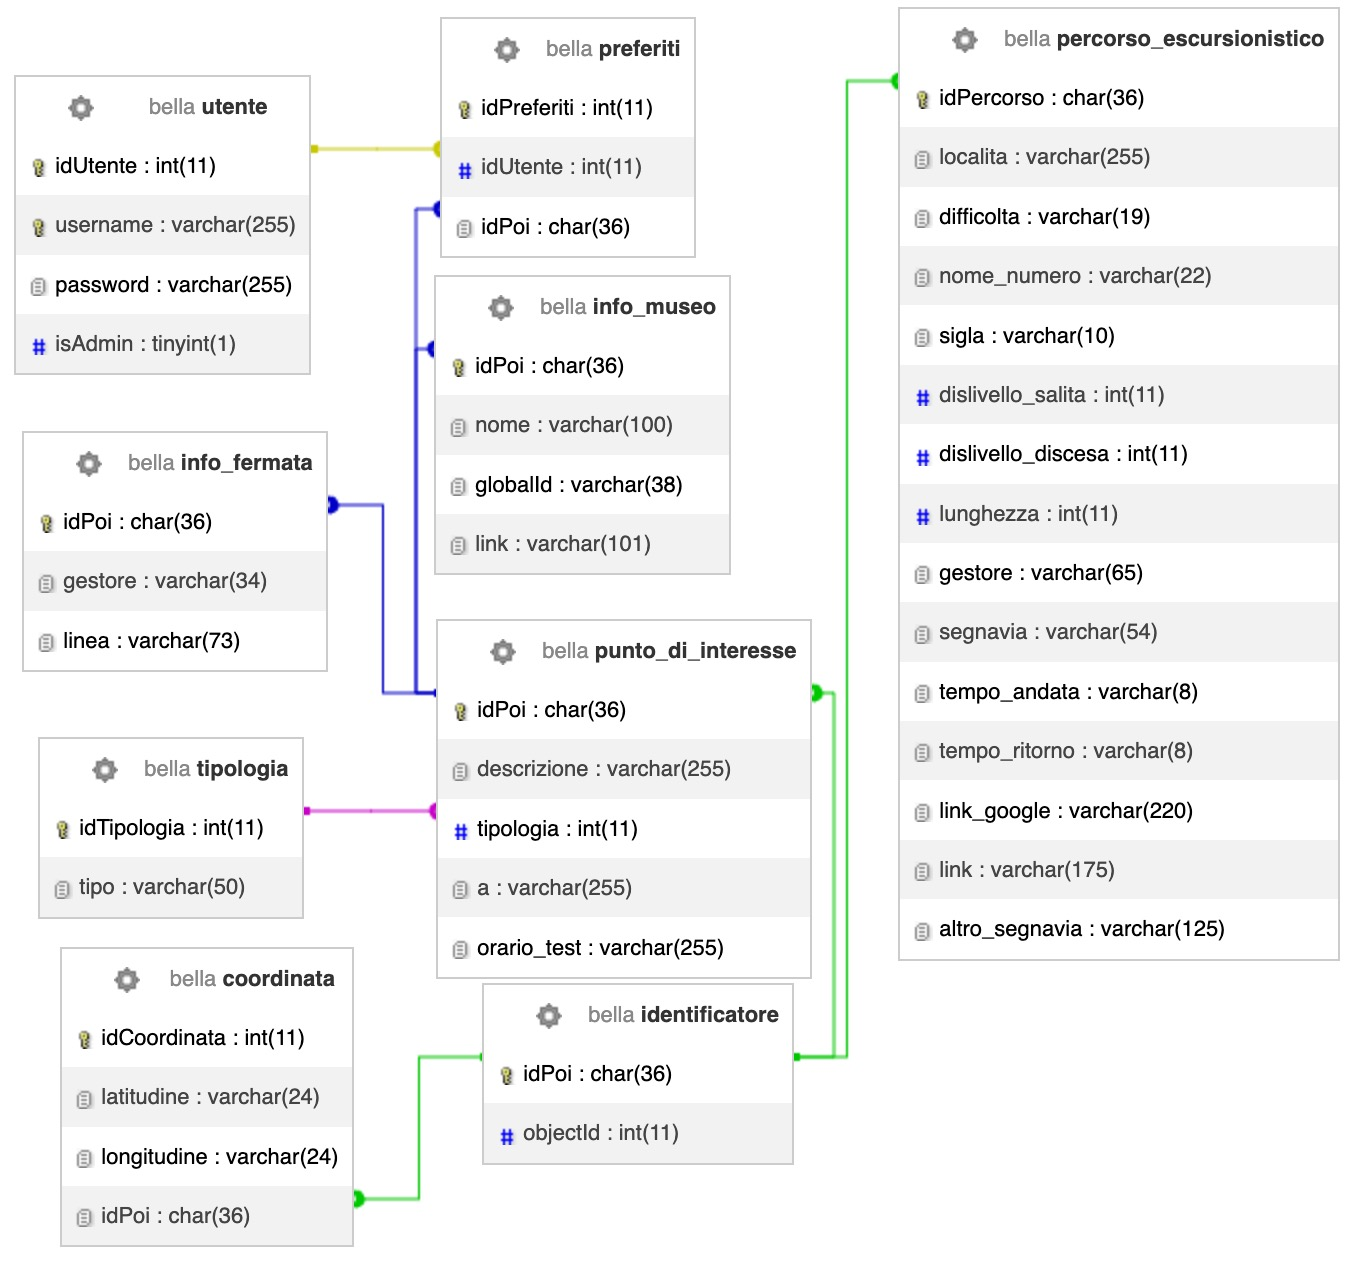
\includegraphics[width=13cm]{images/Database.jpg}
\caption[Struttura del database]{Struttura del database}\label{fig:database}
\end{center}
\end{figure}

\section{Connettere front-end e back-end}
Installato Vue.js, e creato il progetto, per connetterlo al server Apache è stato impostato un proxy, per fare in modo tale che ogni volta che venga fatta richiesta ad una cartella, tale richiesta viene inviata al server Apache ad un percorso specifico. Tutto questo è stato reso fattibile attraverso i file di impostazioni di Vue.js (figura \ref{fig:Webpack}).

\begin{figure}[h]
\begin{center}                      
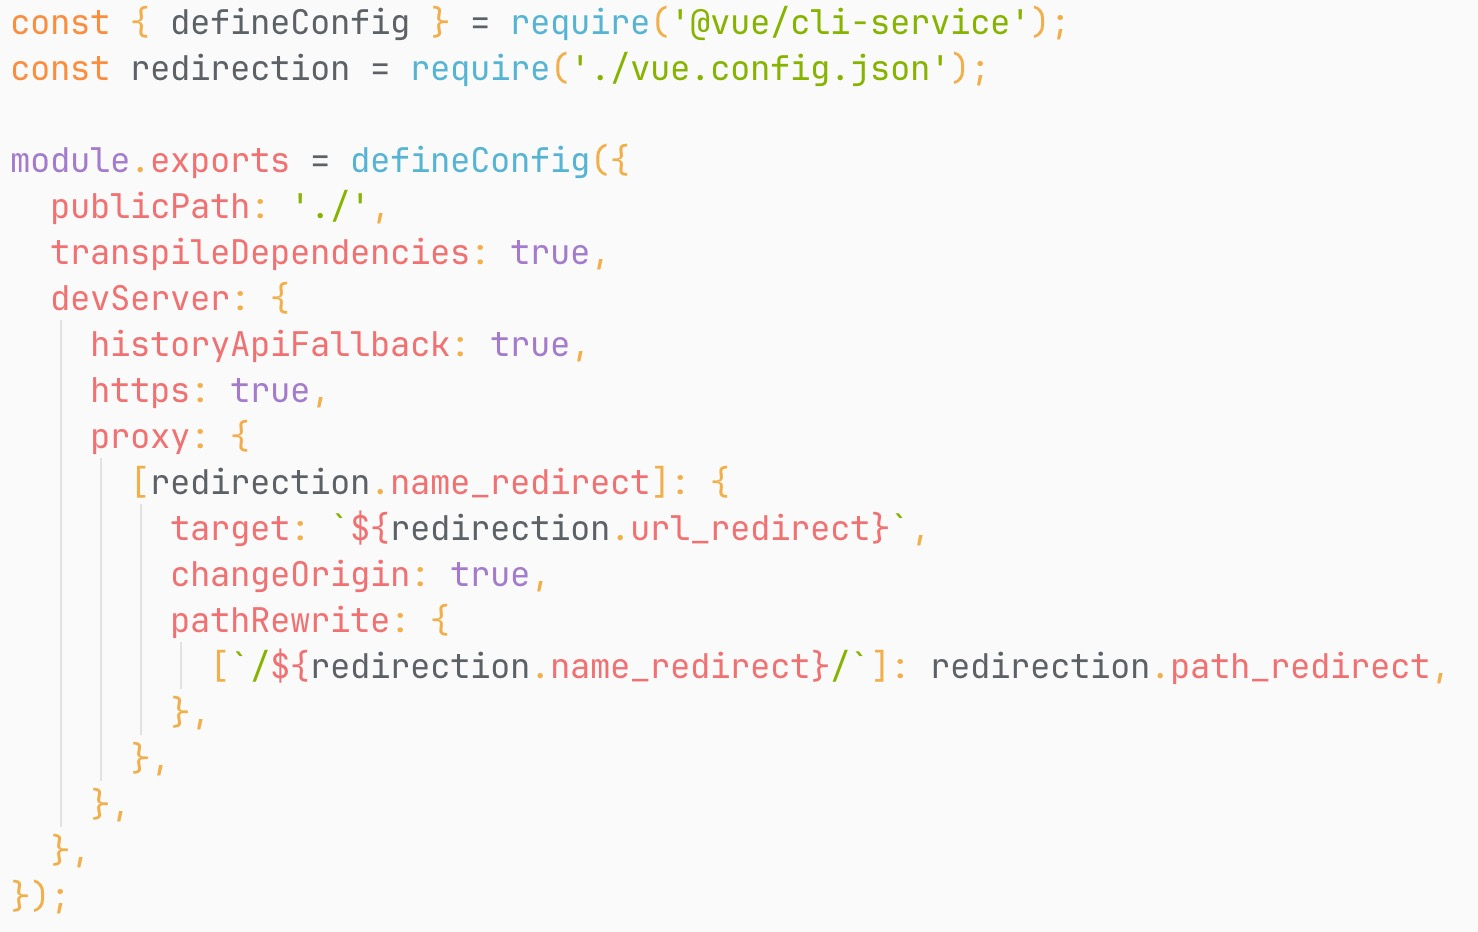
\includegraphics[width=13cm]{images/Webpack.jpg}
\caption[Impostazione web server]{Impostazioni Vue.js}\label{fig:Webpack}
\end{center}
\end{figure}

Al fine di rendere riutilizzabile questo codice, è stato creato inoltre un file \emph{JSON} chiamato ”vue.config.json” che permette di cambiare soltanto i campi principali di questo proxy senza il bisogno di riconfigurare tutto.

\subsection{Implementazione AJAX}
Al fine di fare richieste al server Apache (che successivamente interrogava il database) è stato deciso di creare una personale implementazione di AJAX anziché utilizzare librerie esterne (figura \ref{fig:ajax}).

\begin{figure}[h]
\begin{center}                      
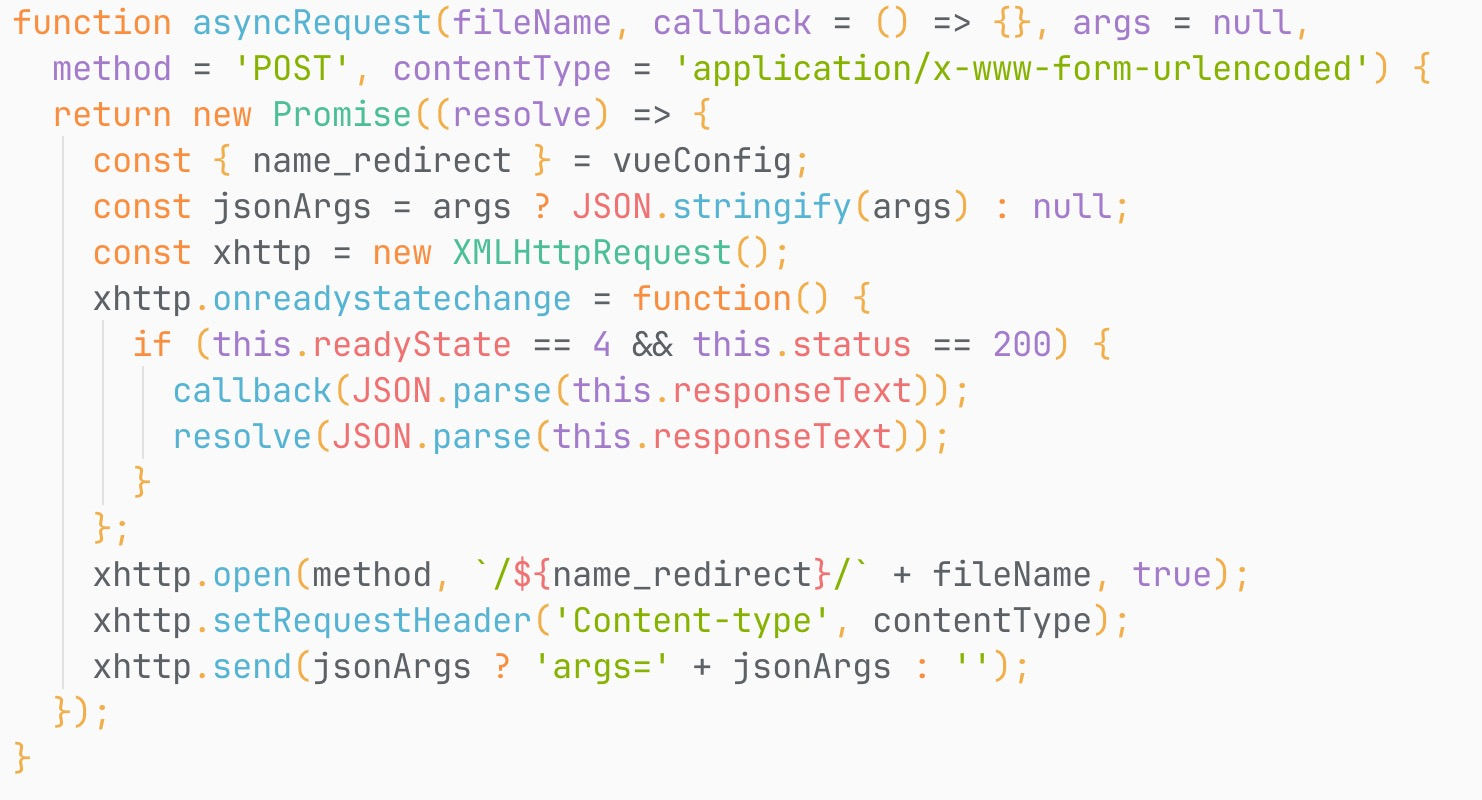
\includegraphics[width=13cm]{images/AJAX.jpg}
\caption[Implementazione di una funzione per le chiamate asincrone]{Implementazione di una funzione per le chiamate asincrone}\label{fig:ajax}
\end{center}
\end{figure}

Come parametri la funzione accetta:
\begin{itemize}
    \item Il nome del file che deve eseguire nel server Apache
    \item La funzione che deve eseguire una volta ritornata la risposta (di base inizializzata a una funzione vuota).
    \item I dati da passare (sotto forma di oggetti Javascript).
    \item Il metodo da utilizzare secondo le RESTful API (di base impostato a ”POST”).
    \item  Un parametro utilizzato per specificare il tipo di dati che stai inviando o ricevendo in una richiesta HTTP (di base impostata a ”application/x-www-form-urlencoded”). 
\end{itemize}

Dopodiché la funzione non fa altro che convertire gli oggetti Javascript da inviare in oggetti JSON. Una volta mandata la richiesta con i parametri passati e ricevuta la risposta senza alcun tipo di errore (quindi con lo stato della richiesta uguale a quattro e con la conferma della stato uguale a duecento) esegue la funzione data in input al metodo passandogli la risposta ottenuta.


\section{Popolamento Database}

Una volta configurato il proxy e creata la struttura del database rimaneva il compito di popolare il database. Come detto in precedenza i dati sono stati forniti sotto forma di file \emph{XML}, tuttavia siccome \emph{MySQL} non supporta questo tipo di file è stata creata una pagina web apposta, accessibile solo agli amministratori, che permette di svuotare e ricaricare il database, mostrando quanto tempo ha impiegato a caricare ogni tipo di punto di interesse (figura \ref{fig:Caricamento_db}).

\begin{figure}[h]
\begin{center}                      
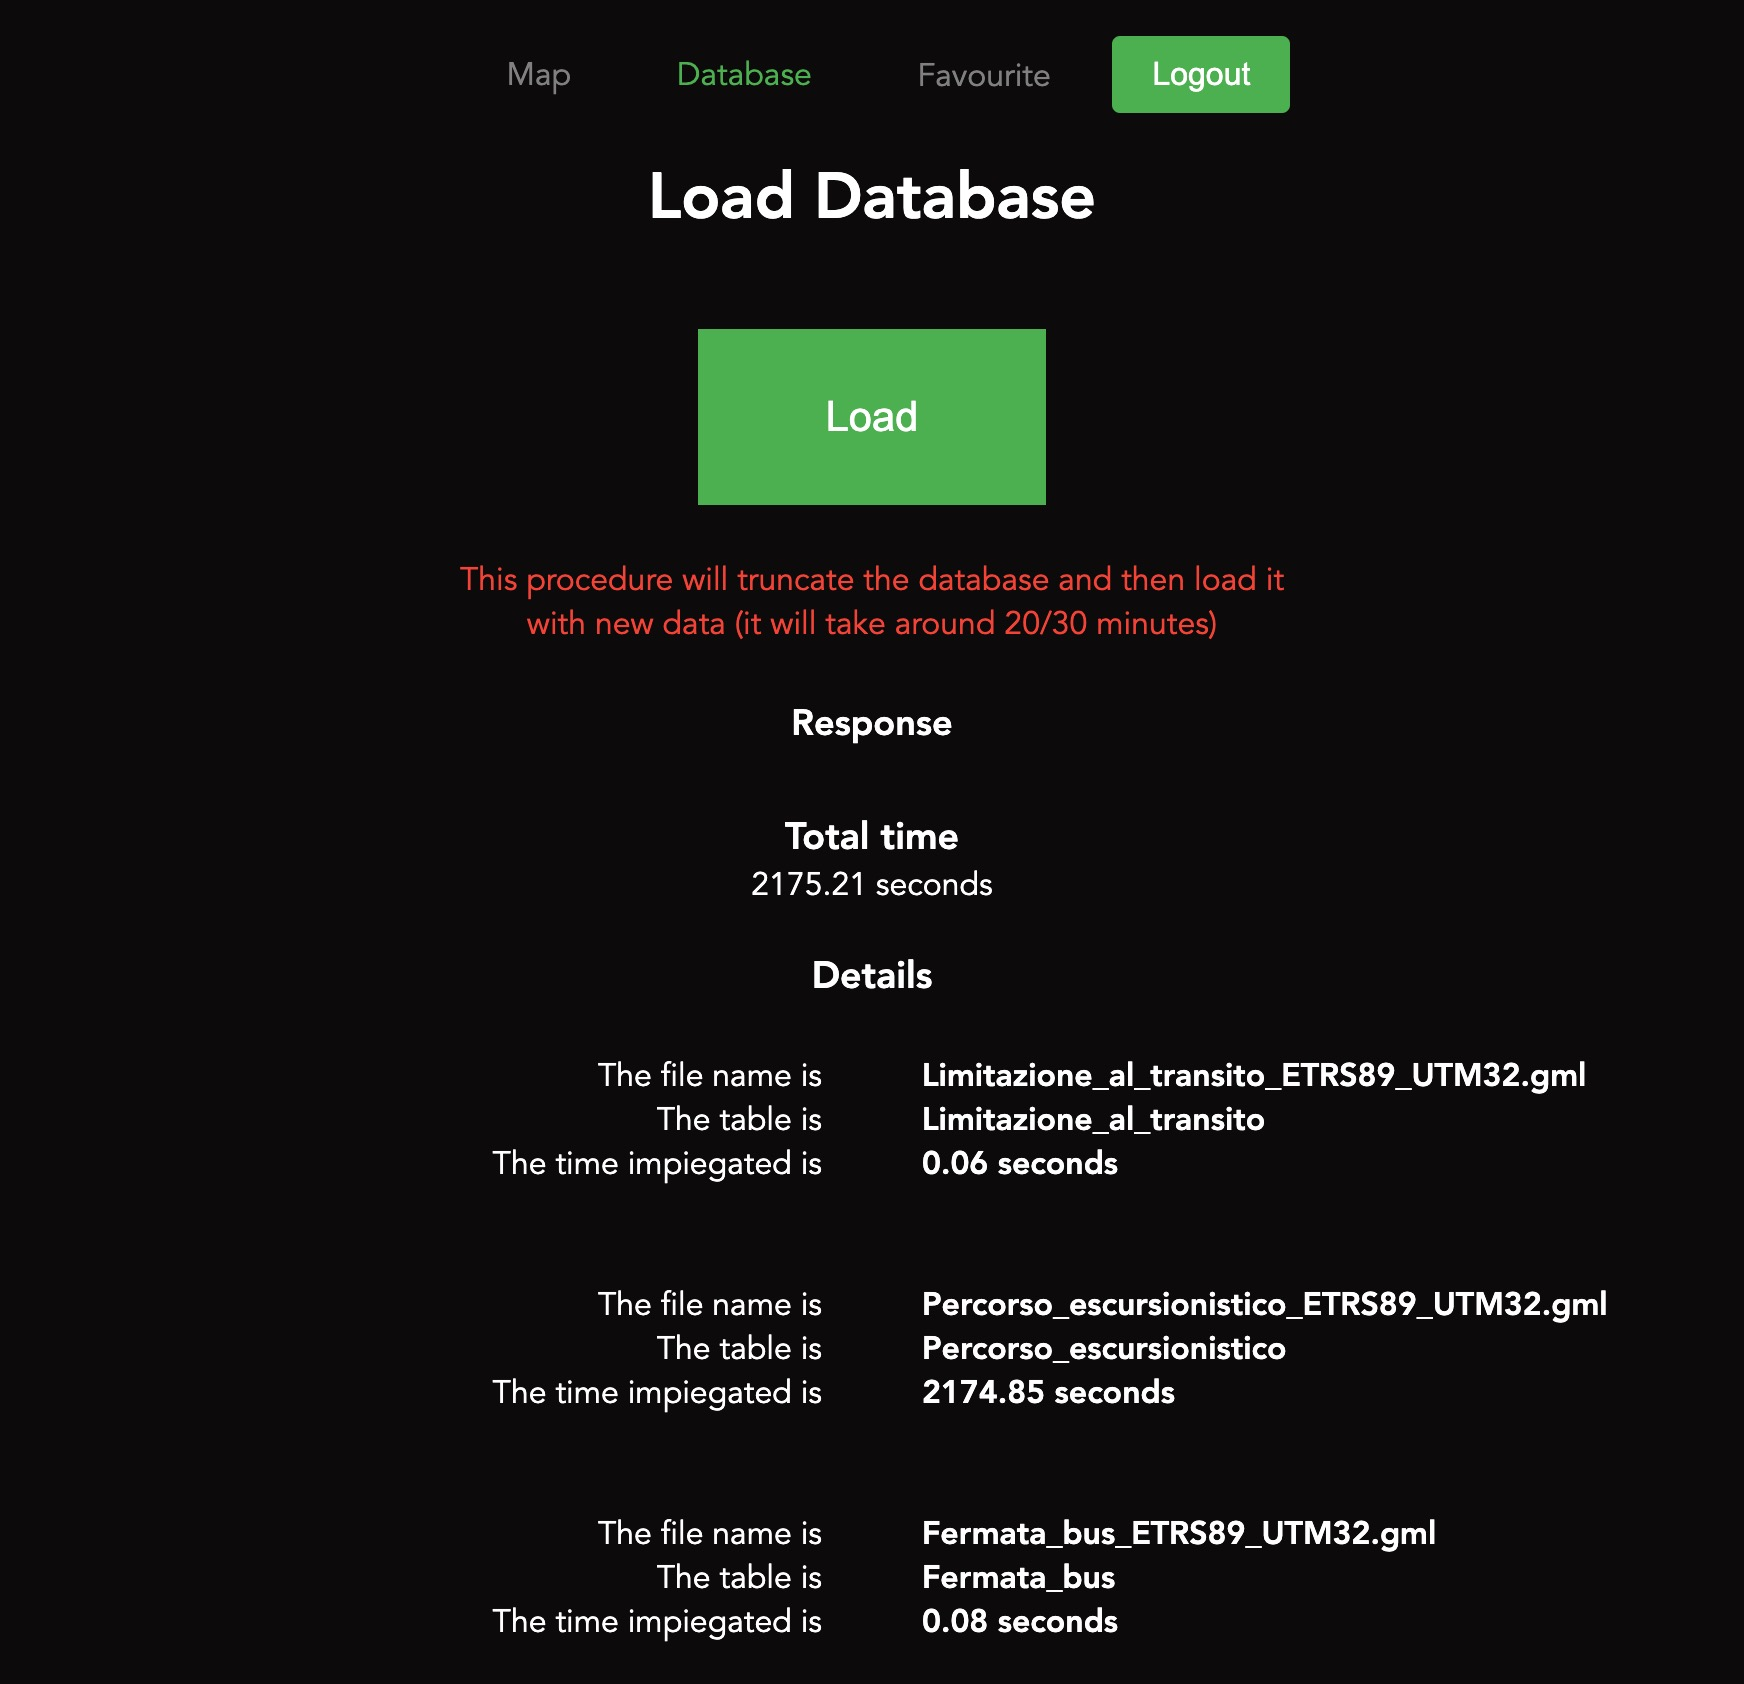
\includegraphics[width=13cm]{images/Caricamento_db.jpg}
\caption[Pagina di caricamento del database]{Pagina di caricamento del database}\label{fig:Caricamento_db}
\end{center}
\end{figure}

\section{Servizio multi pagina di Vue.js}
Una volta installato Vue-Router, un servizio di Vue.js per gestire l'indirizzamento. Dopodiché in un file sono stati creati i vari percorsi che corrispondono alle varie pagine disponibili (figura \ref{fig:route}).

\begin{figure}[h]
\begin{center}                      
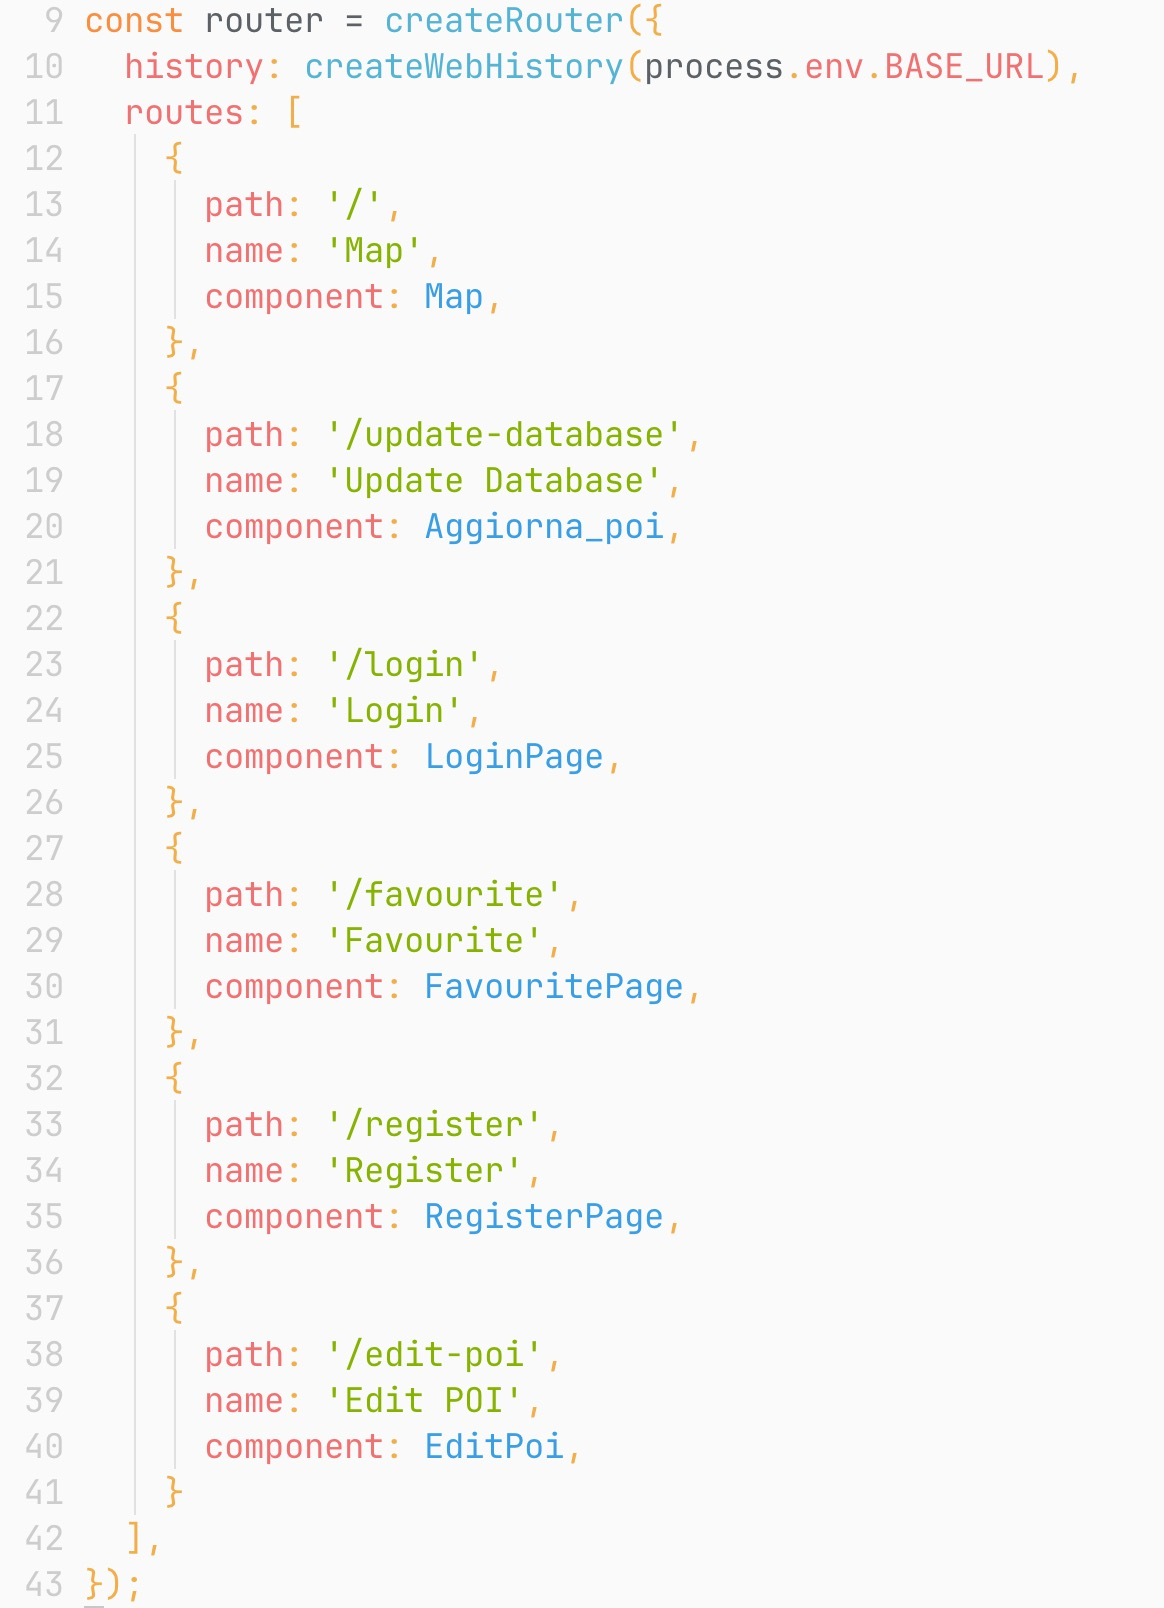
\includegraphics[width=12cm, height=14.5cm]{images/route.jpg}
\caption[Codice per impostare i vari percorsi per le pagine]{Codice per impostare i vari percorsi per le pagine}\label{fig:route}
\end{center}
\end{figure}

\section{Cura del codice}
Prima di iniziare a scrivere codice Javascript nei file Vue, ho voluto impostare uno stile di scrittura del codice utilizzando eslint al fine di avere del codice più pulito. Le regole principale impostate sono visibili in figura \ref{fig:eslint}.

\begin{figure}[h]
\begin{center}                      
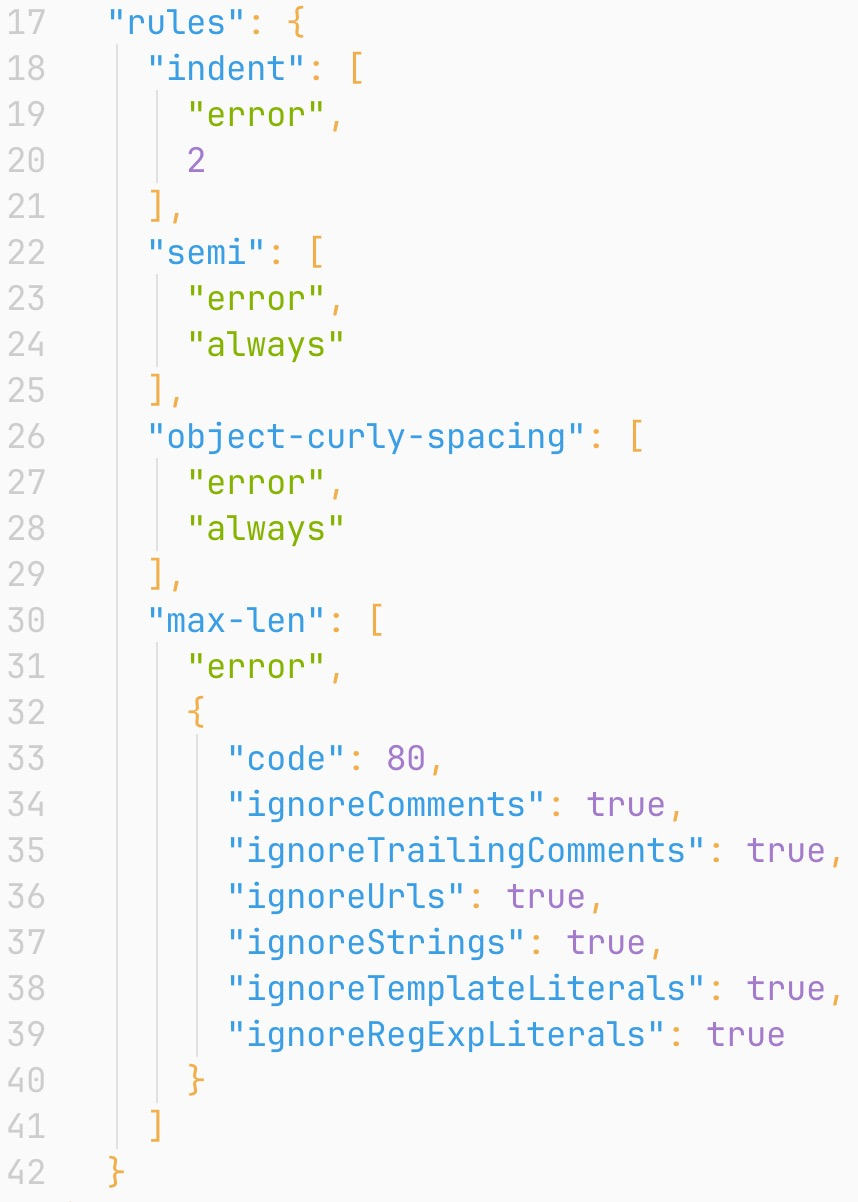
\includegraphics[width=12cm, height=13cm]{images/eslint.jpg}
\caption[Regole principale di eslint]{Regole principale di eslint}\label{fig:eslint}
\end{center}
\end{figure}

Tra queste regole, le principali sono:

\begin{itemize}
    \item La gestione dei ”tab”

    Ogni ”tab” è reso uguale a due spazi, come consigliato dalle
    \href{https://eslint.vuejs.org/}{linee guida di Vue.js}.

    \item Limitazione di caratteri su una riga

    È stato limitato il numero di caratteri su una riga fino ad un limite di 80, per assicurare maggiore leggibilità del codice.
\end{itemize}



\section{Pagina principale}
Appena caricato il database è stato possibile realizzare la pagina principale, che mostra una mappa interattiva della regione ”Emilia-Romagna” evidenziandone i percorsi escursionistici e i punti di interesse (figura \ref{fig:principale}).

\begin{figure}[h]
\begin{center}                      
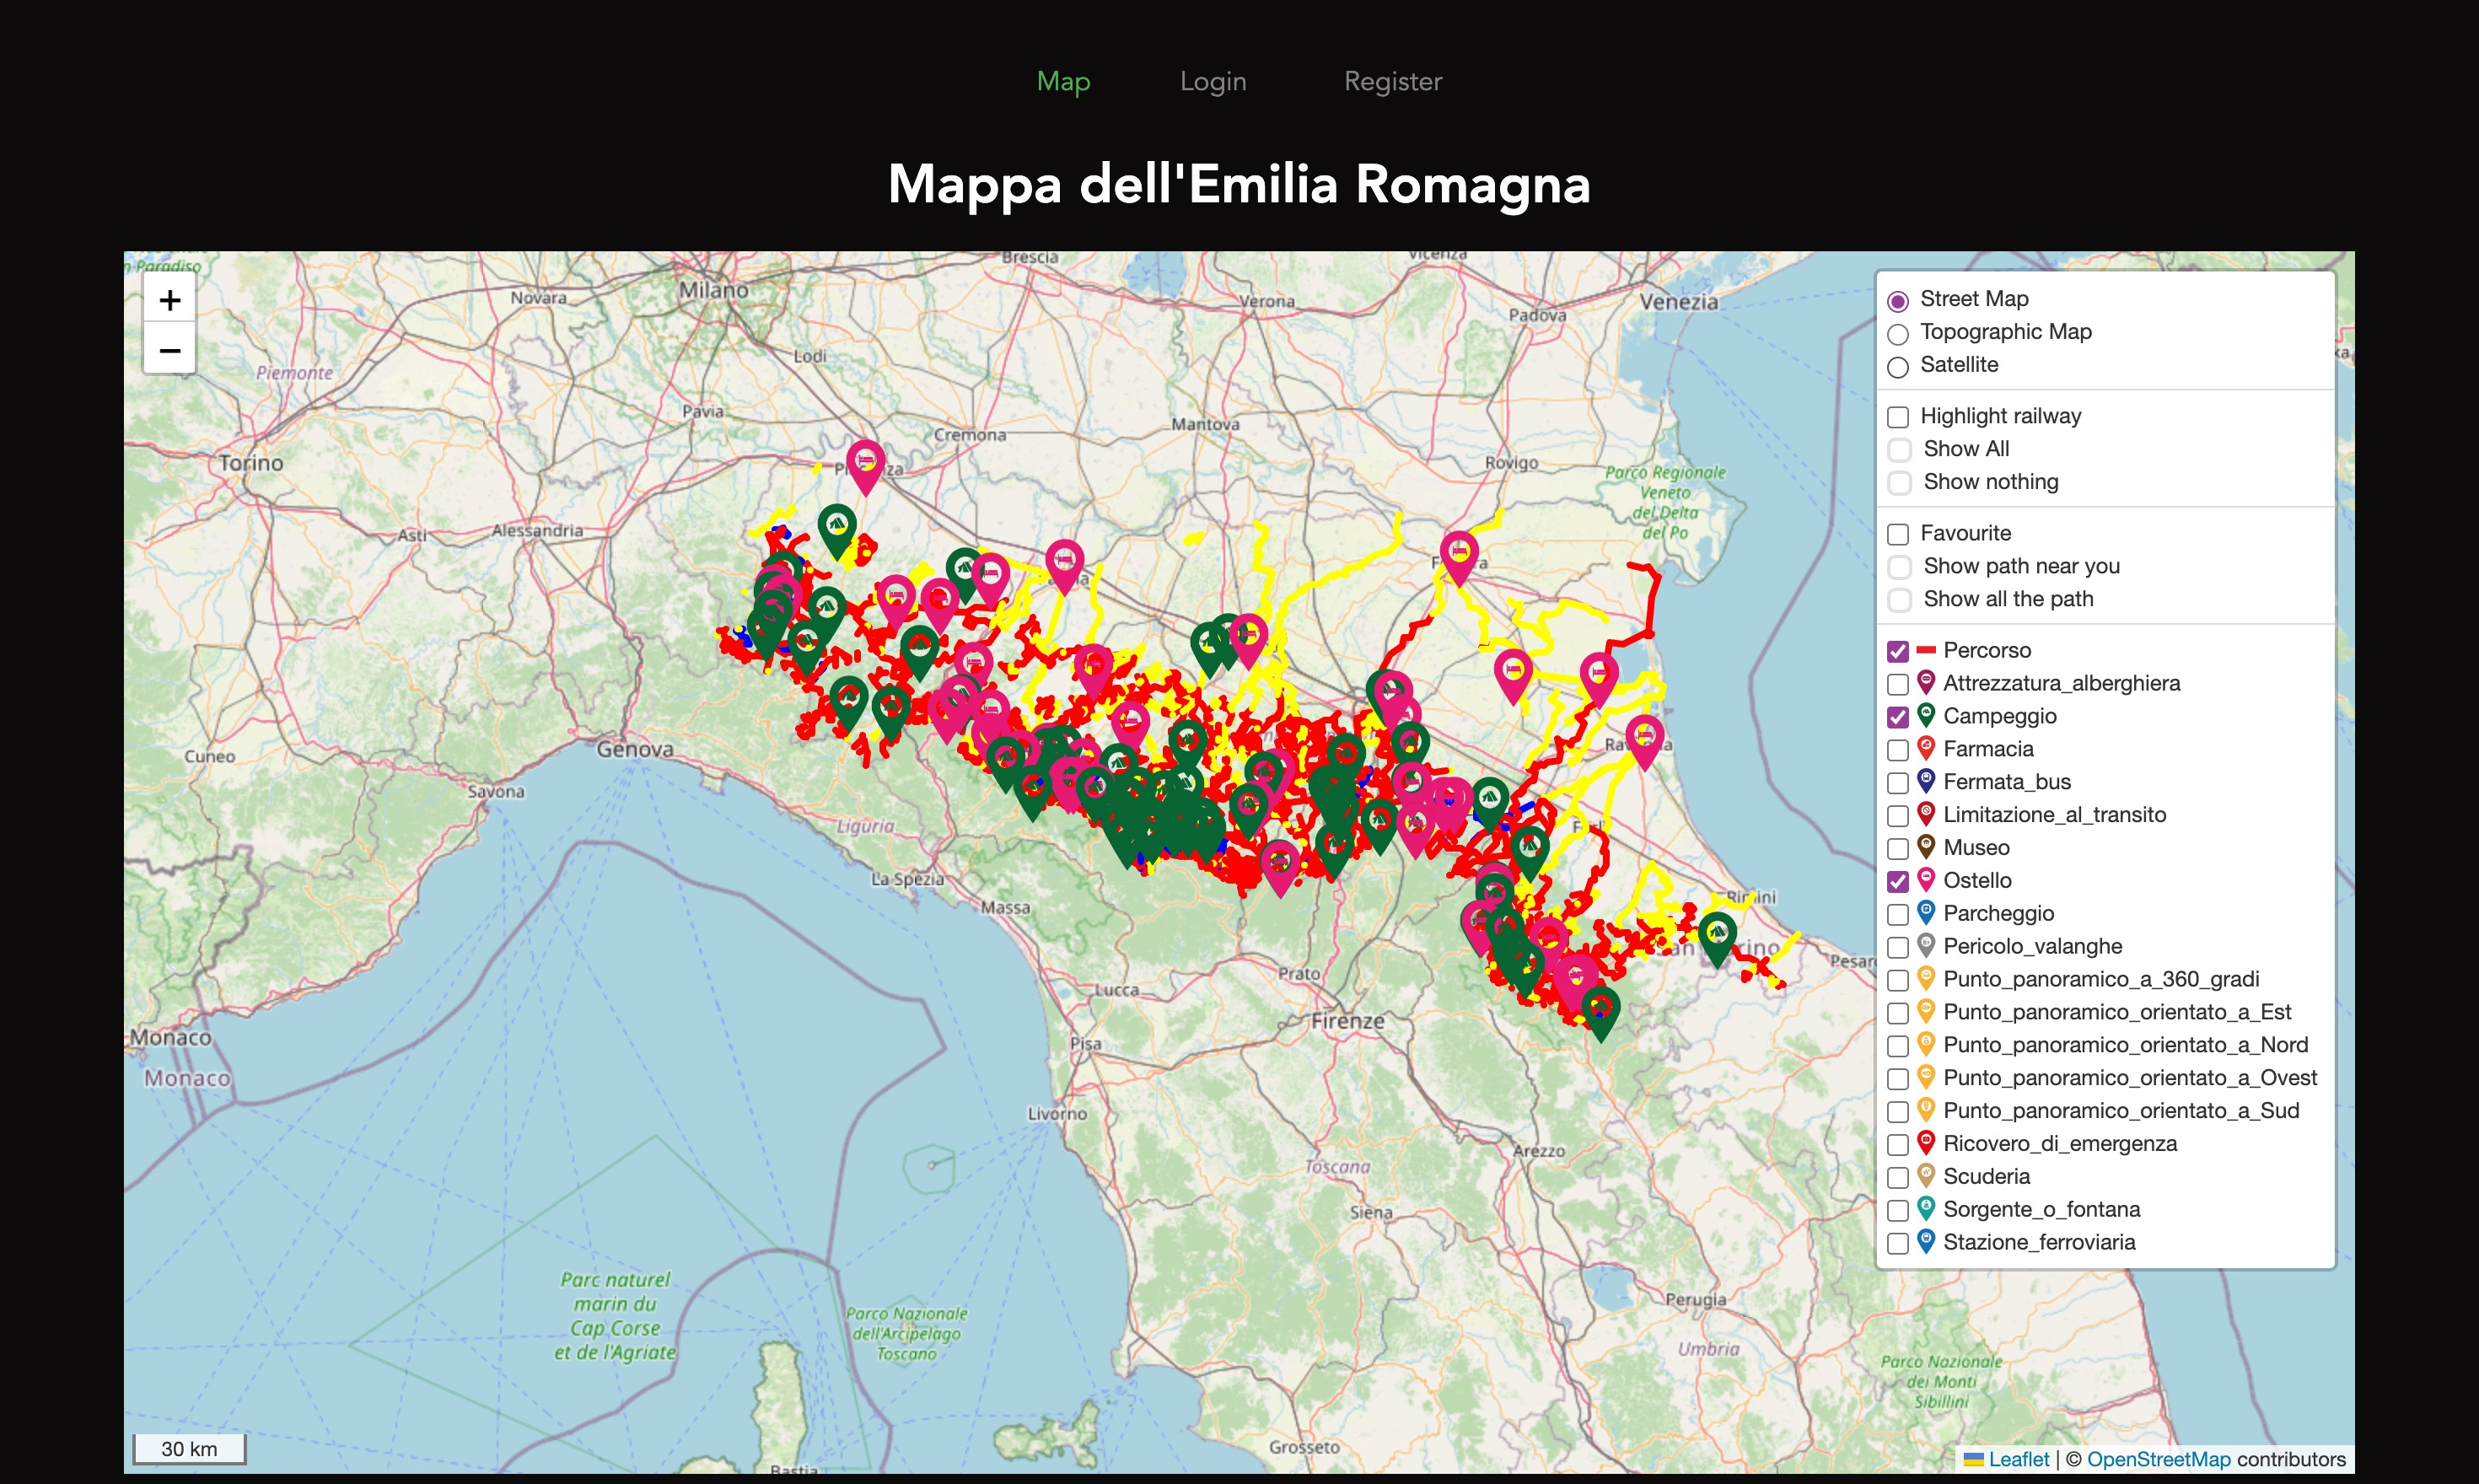
\includegraphics[width=12cm]{images/Schermata_principale.jpg}
\caption[Pagina principale]{Dimostrazione della pagina principale}\label{fig:principale}
\end{center}
\end{figure}

I vari percorsi sono colorati in base alla difficoltà:
\begin{itemize}
    \item I percorsi che sono di tipo ”E - Escursionistico” sono colorati di colore rosso
    \item I percorsi che sono di tipo ”EE - Difficile” sono colorati di colore blu
    \item I percorsi che sono di tipo ”EEA - Attrezzato” sono colorati di colore verde
    \item I percorsi che sono di tipo ”T - Turistico” sono colorati di colore giallo
\end{itemize}

In questa pagina sono presenti vari opzioni nel menù a destra.
Nella prima sezione possiamo scegliere il tipo di mappa che vogliamo mettere come sfondo, e abbiamo tre diverse opzioni:
\begin{itemize}
    \item La prima opzione è di impostare come base la cartina fisica (ed è la scelta preimpostata).
    \item La prima opzione è di impostare come base la cartina topografica.
    \item L'ultima opzione è di impostare come base la mappa satellitare.
\end{itemize}

Nella seconda sezione possiamo scegliere se mostrare tutti i punti di interesse, nasconderli tutti o mettere in risalto i percorsi ferroviari (figura \ref{fig:railway}).

\begin{figure}[h]
\begin{center}                      
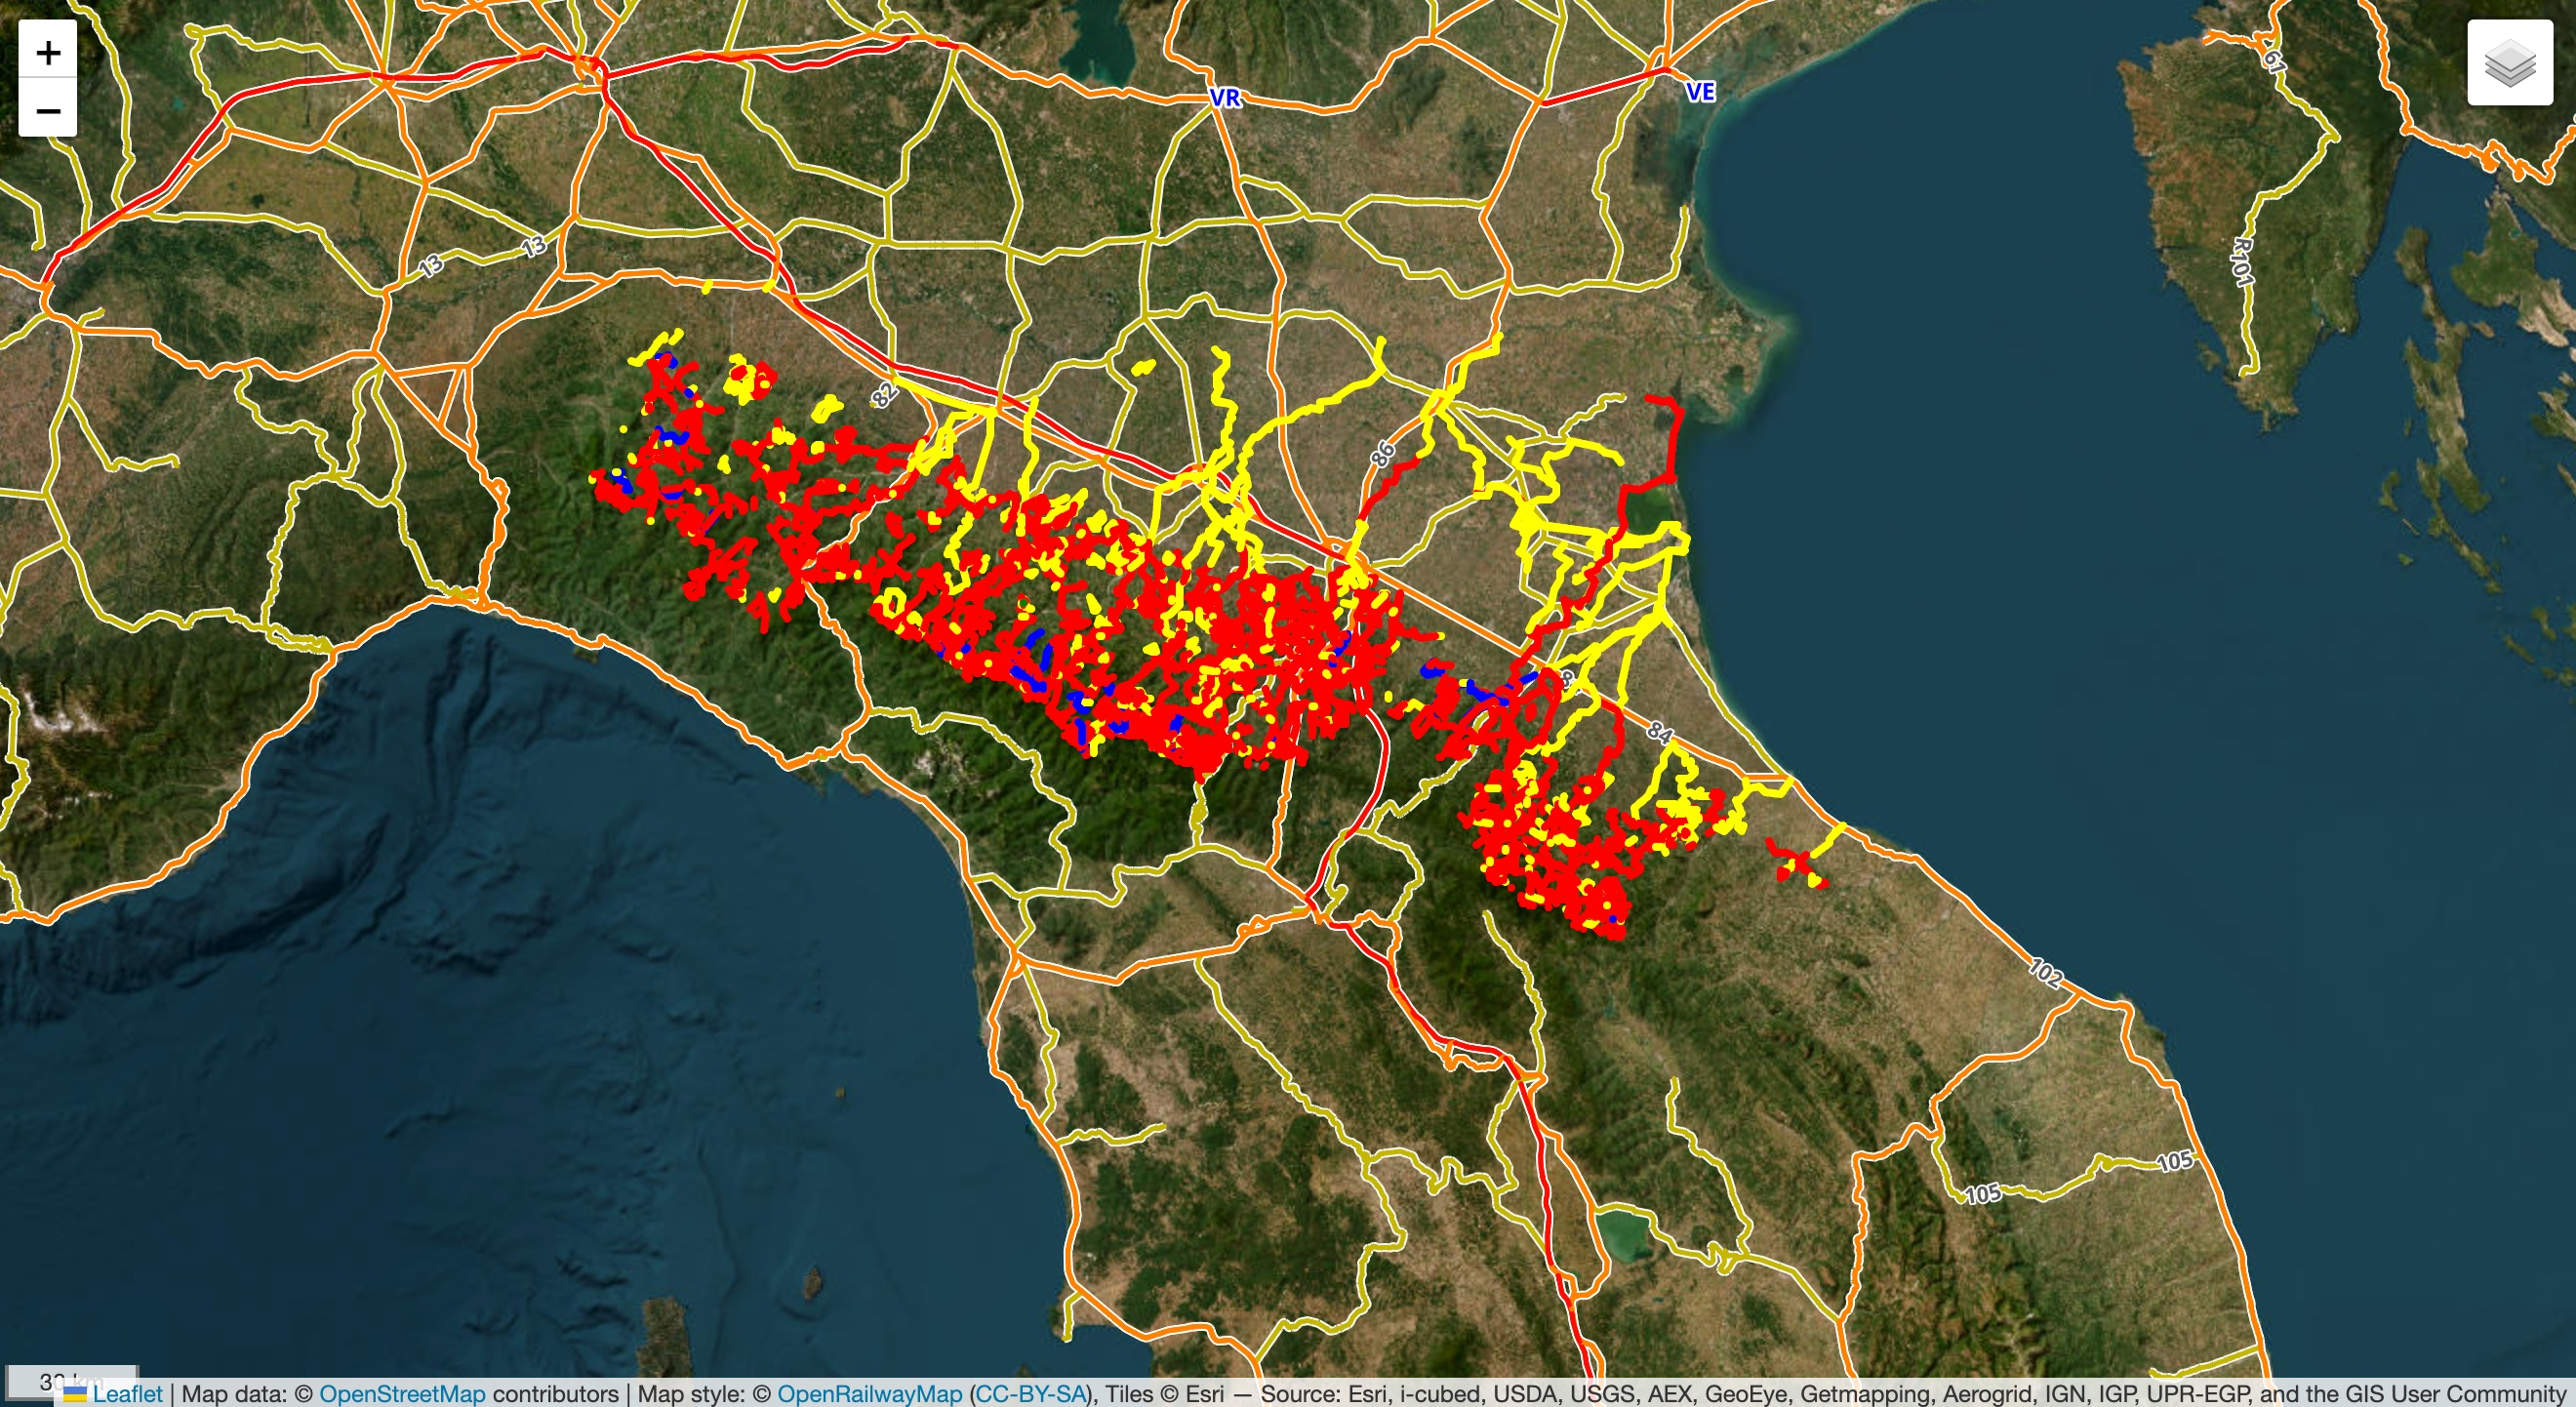
\includegraphics[width=0.7\textwidth]{images/Railway.jpg}
\caption[Mappa satellitare con i percorsi ferroviari evidenziati]{Mappa satellitare con i percorsi ferroviari evidenziati}\label{fig:railway}
\end{center}
\end{figure}

Nella terza sezione del menù possiamo scegliere se mostrare i punti di interesse aggiunti come preferiti (solo nel caso in cui l'utente abbia effettuato la registrazione e l'accesso), se mostrare tutti i percorsi della regione o se mostrare solo i percorsi vicini alla posizione dell'utente.

Infine nell'ultima sezione è possibile scegliere quali punti di interesse mostrare e nascondere.

\section{Geo localizzazione}

L'applicazione permette inoltre di mostrare solamente i  percorsi nelle vicinanze in un raggio di 40km. Per calcolare i quali percorsi mostrare viene utilizzata la formula di Haversine che ci permette di calcolare in modo efficiente le distanze geografiche sulla superficie terrestre~\cite{Haversine}.

La formula di Haversine è espressa come segue:

\begin{align*}
a &= \sin^2\left(\frac{\Delta\phi}{2}\right) + \cos(\phi_1) \cdot \cos(\phi_2) \cdot \sin^2\left(\frac{\Delta\lambda}{2}\right) \\
c &= 2 \cdot \text{atan2}\left(\sqrt{a}, \sqrt{1-a}\right) \\
d &= R \cdot c
\end{align*}

Dove:
\begin{align*}
\Delta\phi & \text{ è la differenza di latitudine tra i due punti.} \\
\Delta\lambda & \text{ è la differenza di longitudine tra i due punti.} \\
\phi_1 & \text{ è la latitudine del primo punto.} \\
\phi_2 & \text{ è la latitudine del secondo punto.} \\
R & \text{ è il raggio della Terra (approssimativamente 6,371 km).}
\end{align*}

I valori ottenuti sono:
\begin{itemize}
    \item \emph{a} che è un valore che viene utilizzato successivamente per calcolare altre componenti.

    \item \emph{c} che rappresenta l'angolo calcolato usando il valore $\alpha$ e la funzione atan2. Questo angolo è utilizzato per calcolare la distanza sulla superficie terrestre tra i due punti.

    \item \emph{d} che rappresenta la distanza sulla superficie terrestre tra i due punti, misurata in unità di lunghezza specificate dal raggio terrestre $R$. Questa è la distanza effettiva tra i due punti che stai cercando di calcolare.
\end{itemize}

Quindi infine viene controllato il valore \emph{d} che rappresenta la distanza tra le coordinate del percorso che si vuole mostrare e le coordinate della posizione dell'utente(figura \ref{fig:vicina}).

\begin{figure}[h]
\begin{center}                      
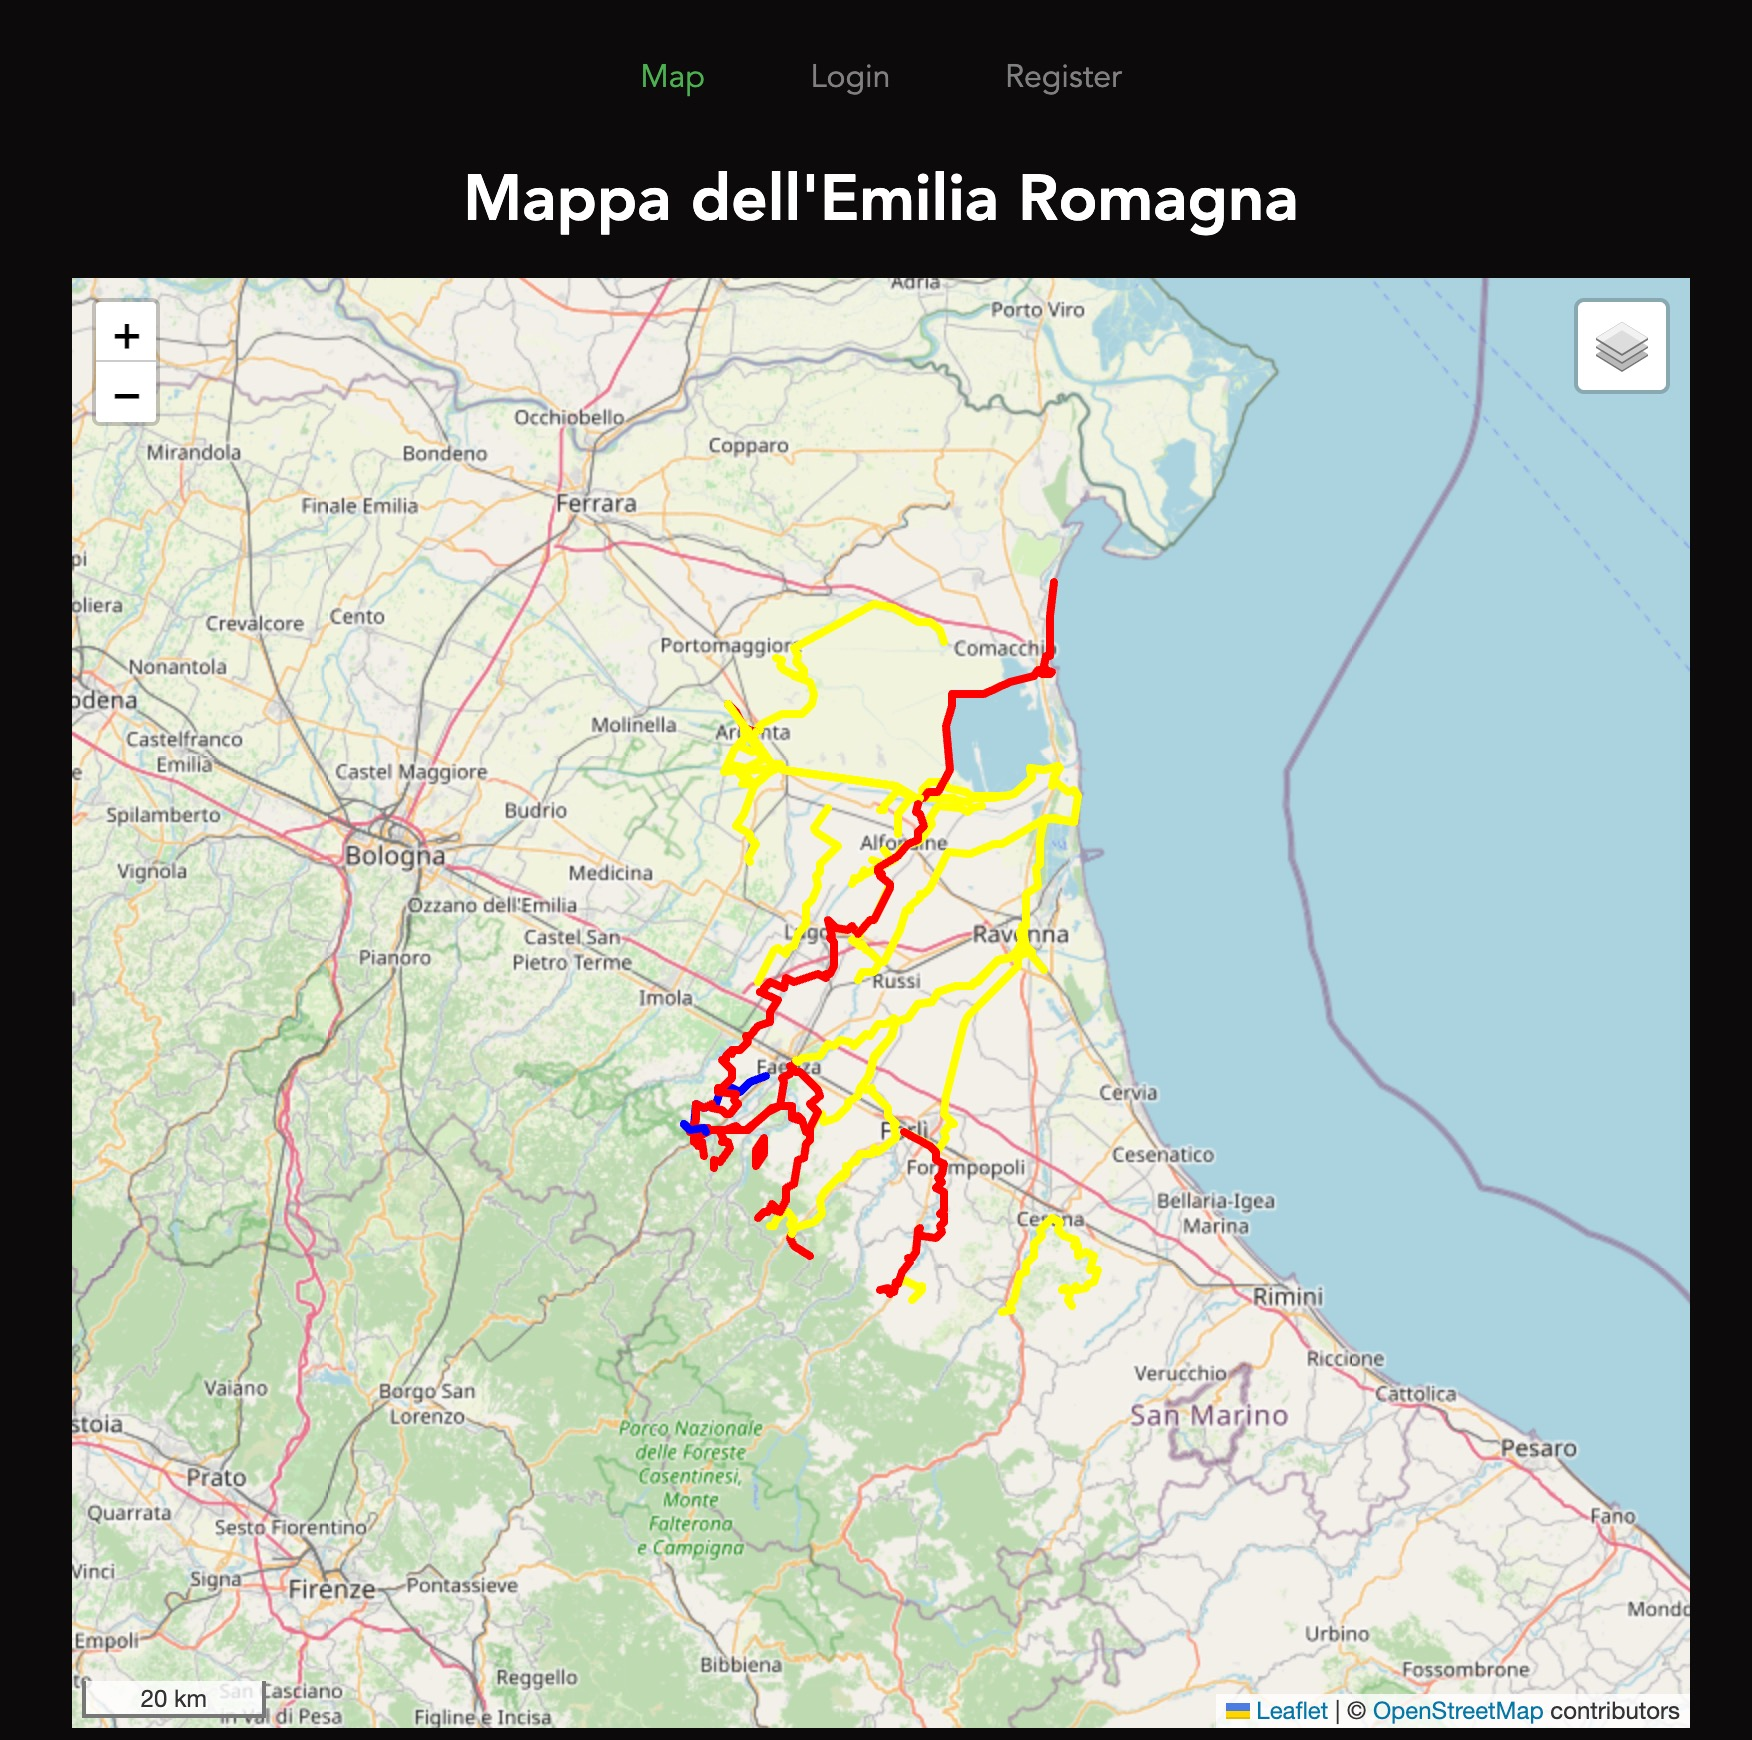
\includegraphics[width=0.7\textwidth]{images/Mappa_vicina.jpg}
\caption[Dimostrazione funzionamento mappa]{Dimostrazione cartina con percorsi vicini all'utente (test effettuato nel centro della città di Ravenna)}\label{fig:vicina}
\end{center}
\end{figure}


\section{Informazioni sui percorsi}
È possibile ottenere informazioni su ogni singolo percorso escursionistico cliccandoci sopra, come dimostrato in figura \ref{fig:info}.

\begin{figure}[h]
\begin{center}                      
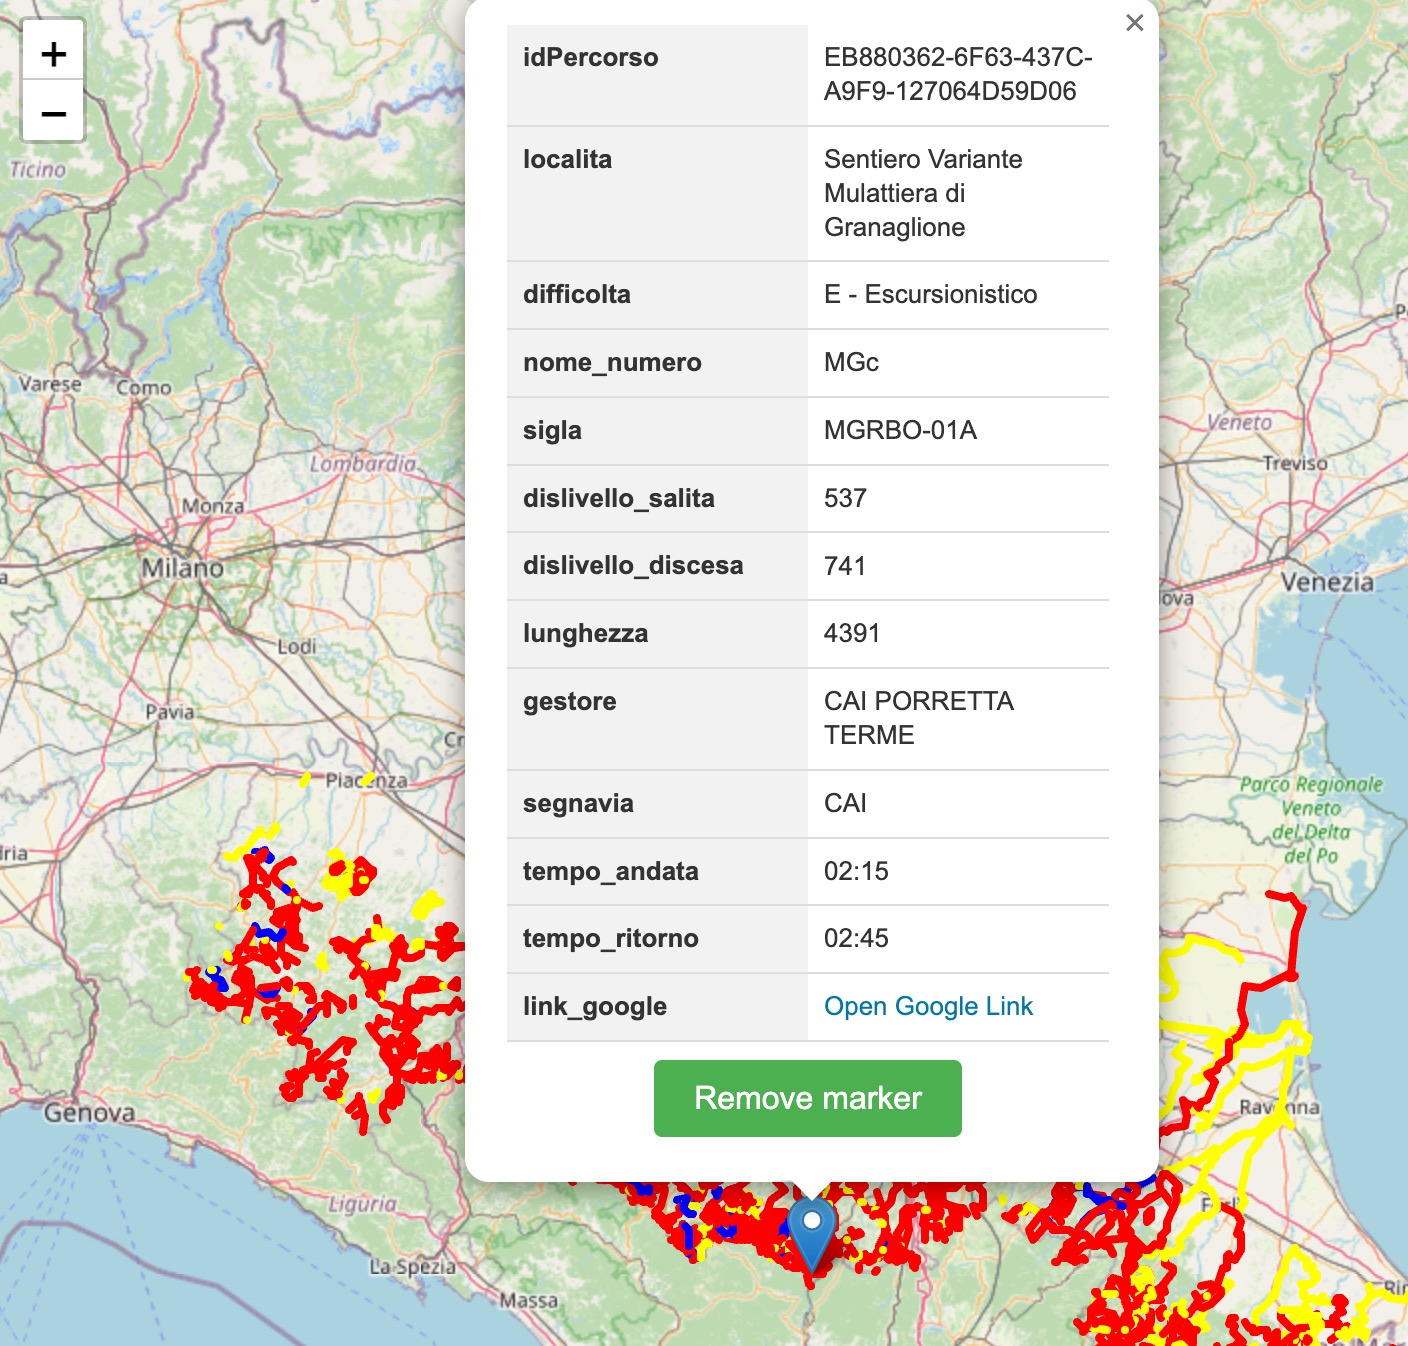
\includegraphics[width=12cm]{images/Informazioni percorso.jpg}
\caption[Dimostrazione informazioni mappa]{Informazioni di un percorso}\label{fig:info}
\end{center}
\end{figure}

\section{Registrazione e accesso}
È possibile registrarsi (figura \ref{fig:registrazione}) e eseguire l'accesso (figura \ref{fig:login}) al fine di aggiungere informazioni sui punti di interesse o di creare una lista di punti di interesse preferiti.

\begin{figure}[h]
    \centering
    \begin{minipage}{0.40\textwidth}
        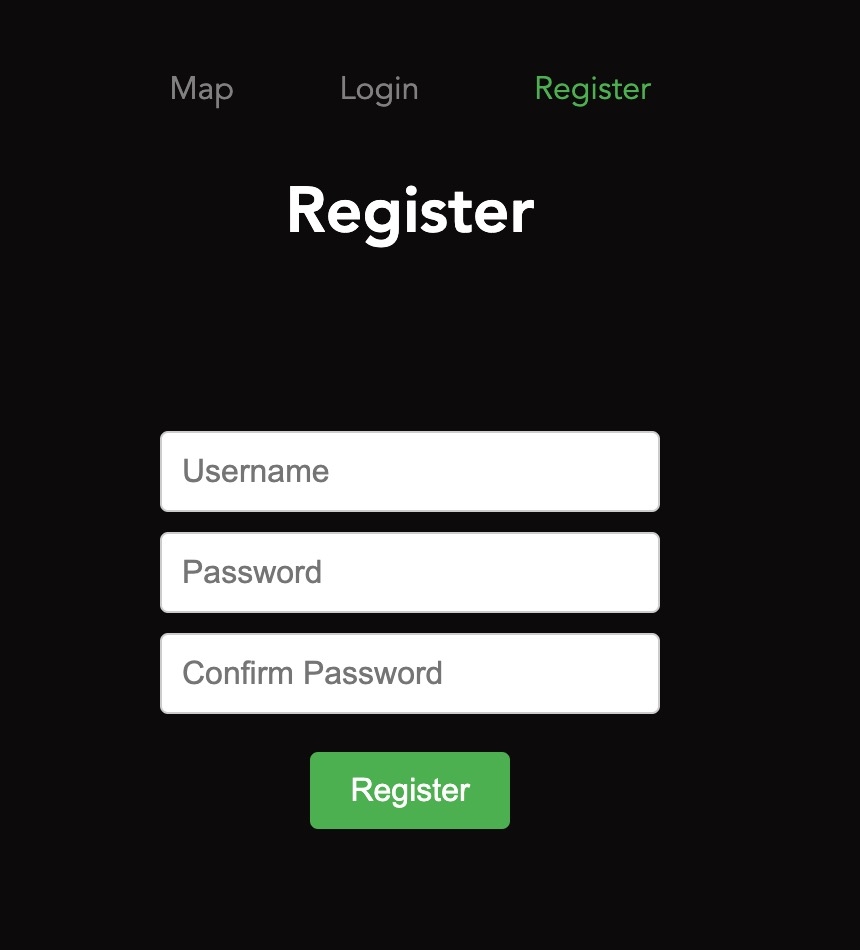
\includegraphics[width=\textwidth]{images/Registrazione.jpg}
        \caption[Pagina di registrazione]{Pagina di registrazione}
        \label{fig:registrazione}
    \end{minipage}

    \vspace{0.6cm}

    \begin{minipage}{0.40\textwidth}
        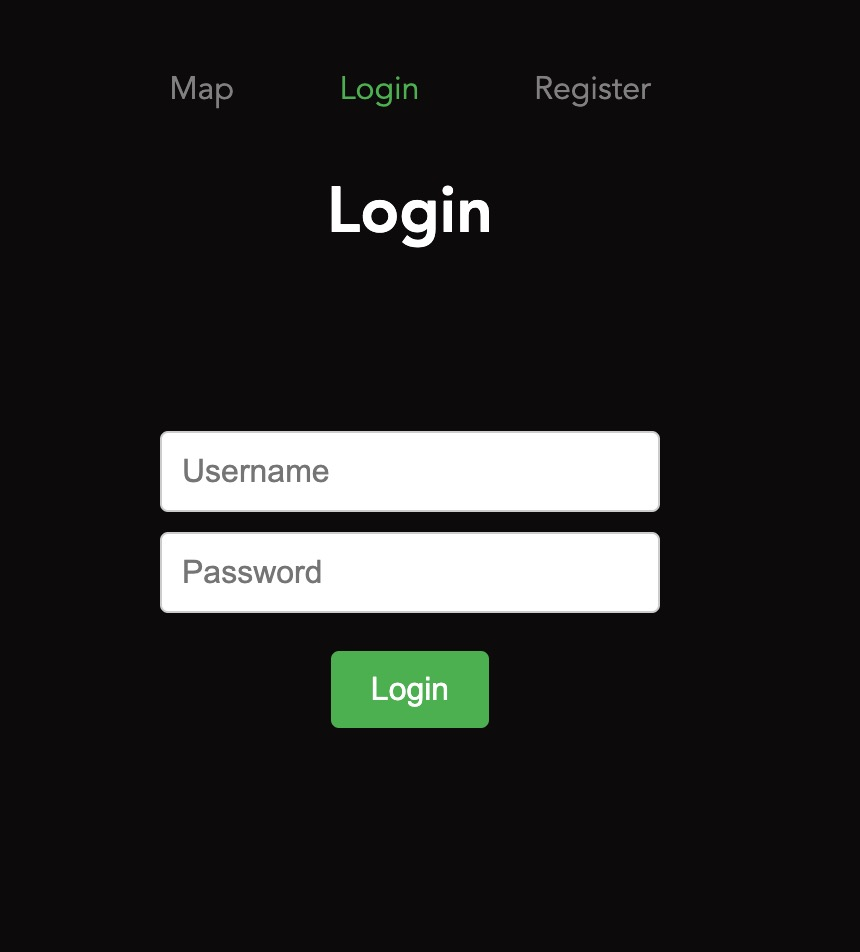
\includegraphics[width=\textwidth]{images/Login.jpg}
        \caption[Pagina per effettuare l'accesso]{Pagina per effettuare l'accesso}
        \label{fig:login}
    \end{minipage}
\end{figure}

\section{Informazioni sui punti di interesse}
Nel caso in cui l'utente clicchi su un punto di interesse è possibile vedere le sue informazioni. Se l'utente ha effettuato l'accesso è inoltre possibile aggiungere altre informazioni e aggiungere il punto nella lista dei punti preferiti (figura \ref{fig:info_punto}).

\begin{figure}[h]
\begin{center} 
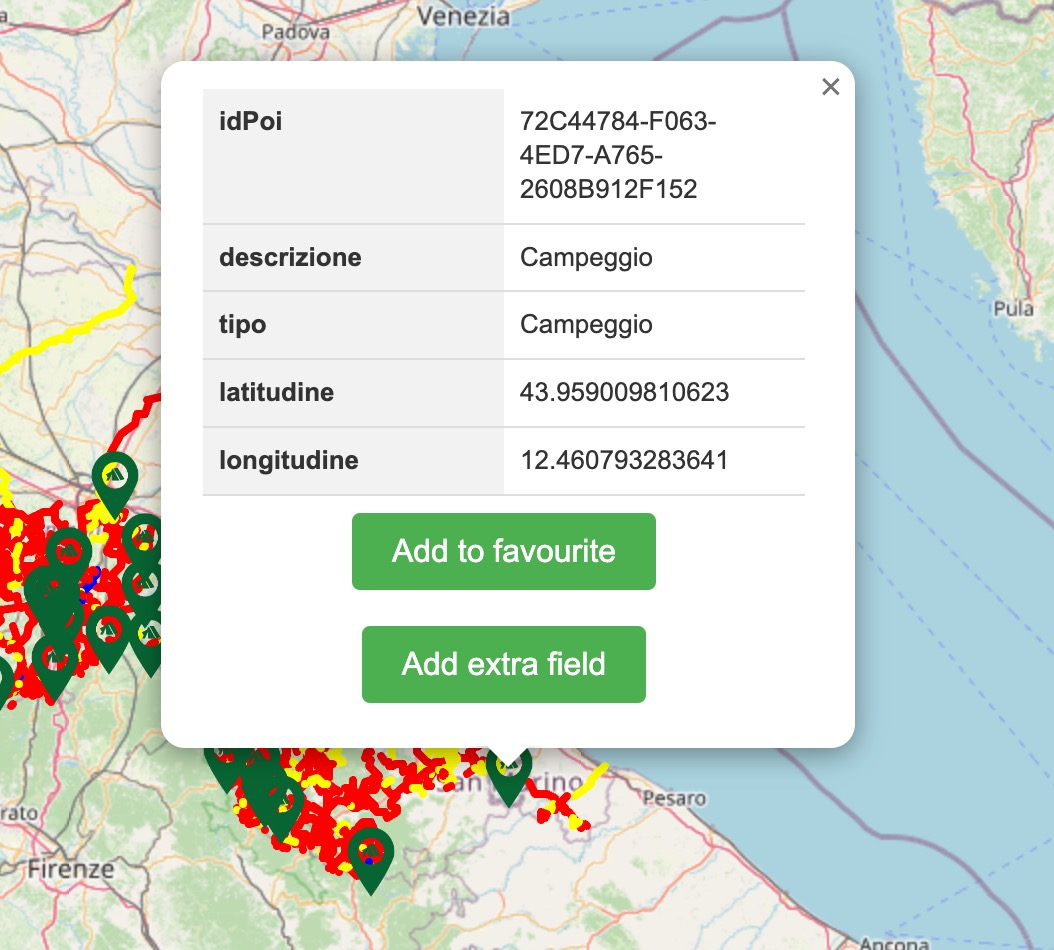
\includegraphics[width=12cm]{images/Info punto.jpg}
\caption[Informazioni di un percorso]{Informazioni di un percorso}\label{fig:info_punto}
\end{center}
\end{figure}

\section{Pagina dei preferiti}

Una volta che l'utente ha eseguito l'accesso e ha aggiunto dei punti di interesse nella sua lista dei preferiti, è possibile vedere una pagina (figura \ref{fig:preferiti}) che mostri tutte le informazioni su questi punti, insieme alla possibilità di filtrarli.

\begin{figure}[h]
\begin{center} 
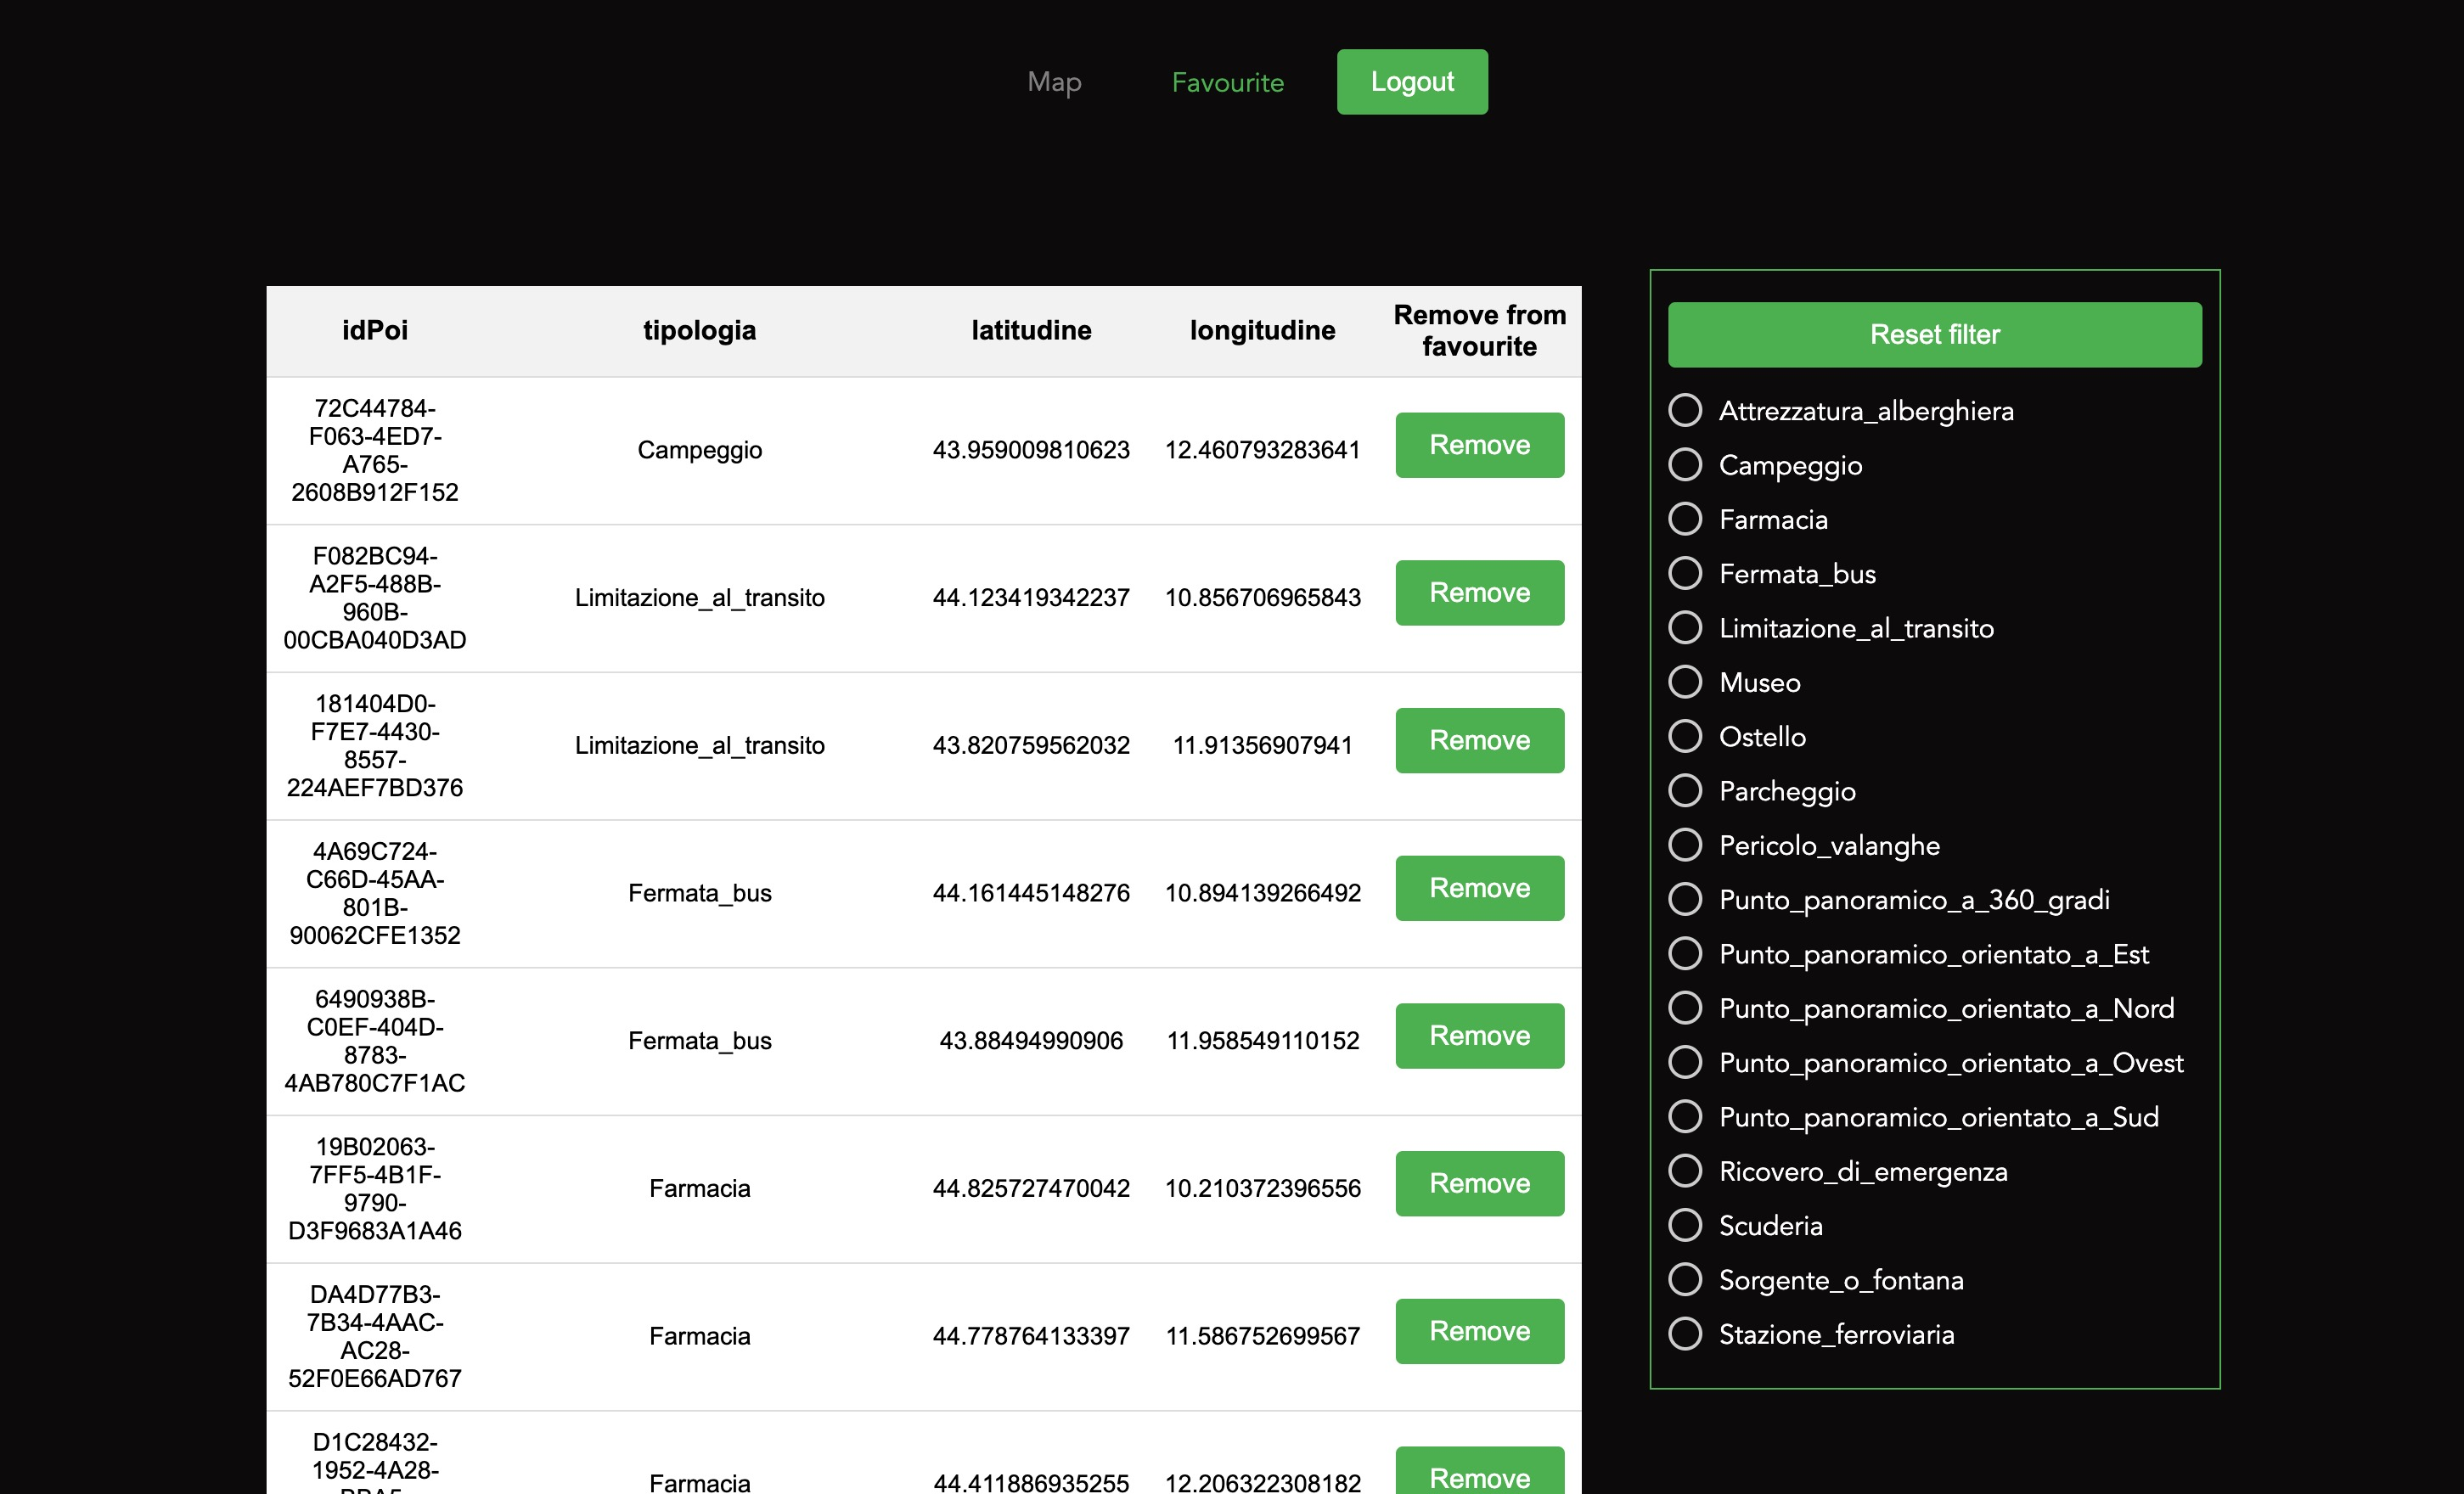
\includegraphics[width=13cm]{images/Favourite page.jpg}
\caption[Pagina dei preferiti]{Pagina dei preferiti}\label{fig:preferiti}
\end{center}
\end{figure}


Da questa pagina è possibile vedere l'identificativo di ogni punto, che tipo di punto di interesse sia e le sue coordinate. Inoltre questa pagina permette di rimuovere ogni elemento dalla lista dei preferiti.

\section{Aggiungere informazioni ai punti}
Una volta che l'utente è registrato può aggiungere informazioni su ogni punto di interesse (come visibile in figura \ref{fig:info_punto}). La pagina da cui eseguire questa operazione appare come raffigurato in figura \ref{fig:extra_field}.

\begin{figure}[h]
\begin{center} 
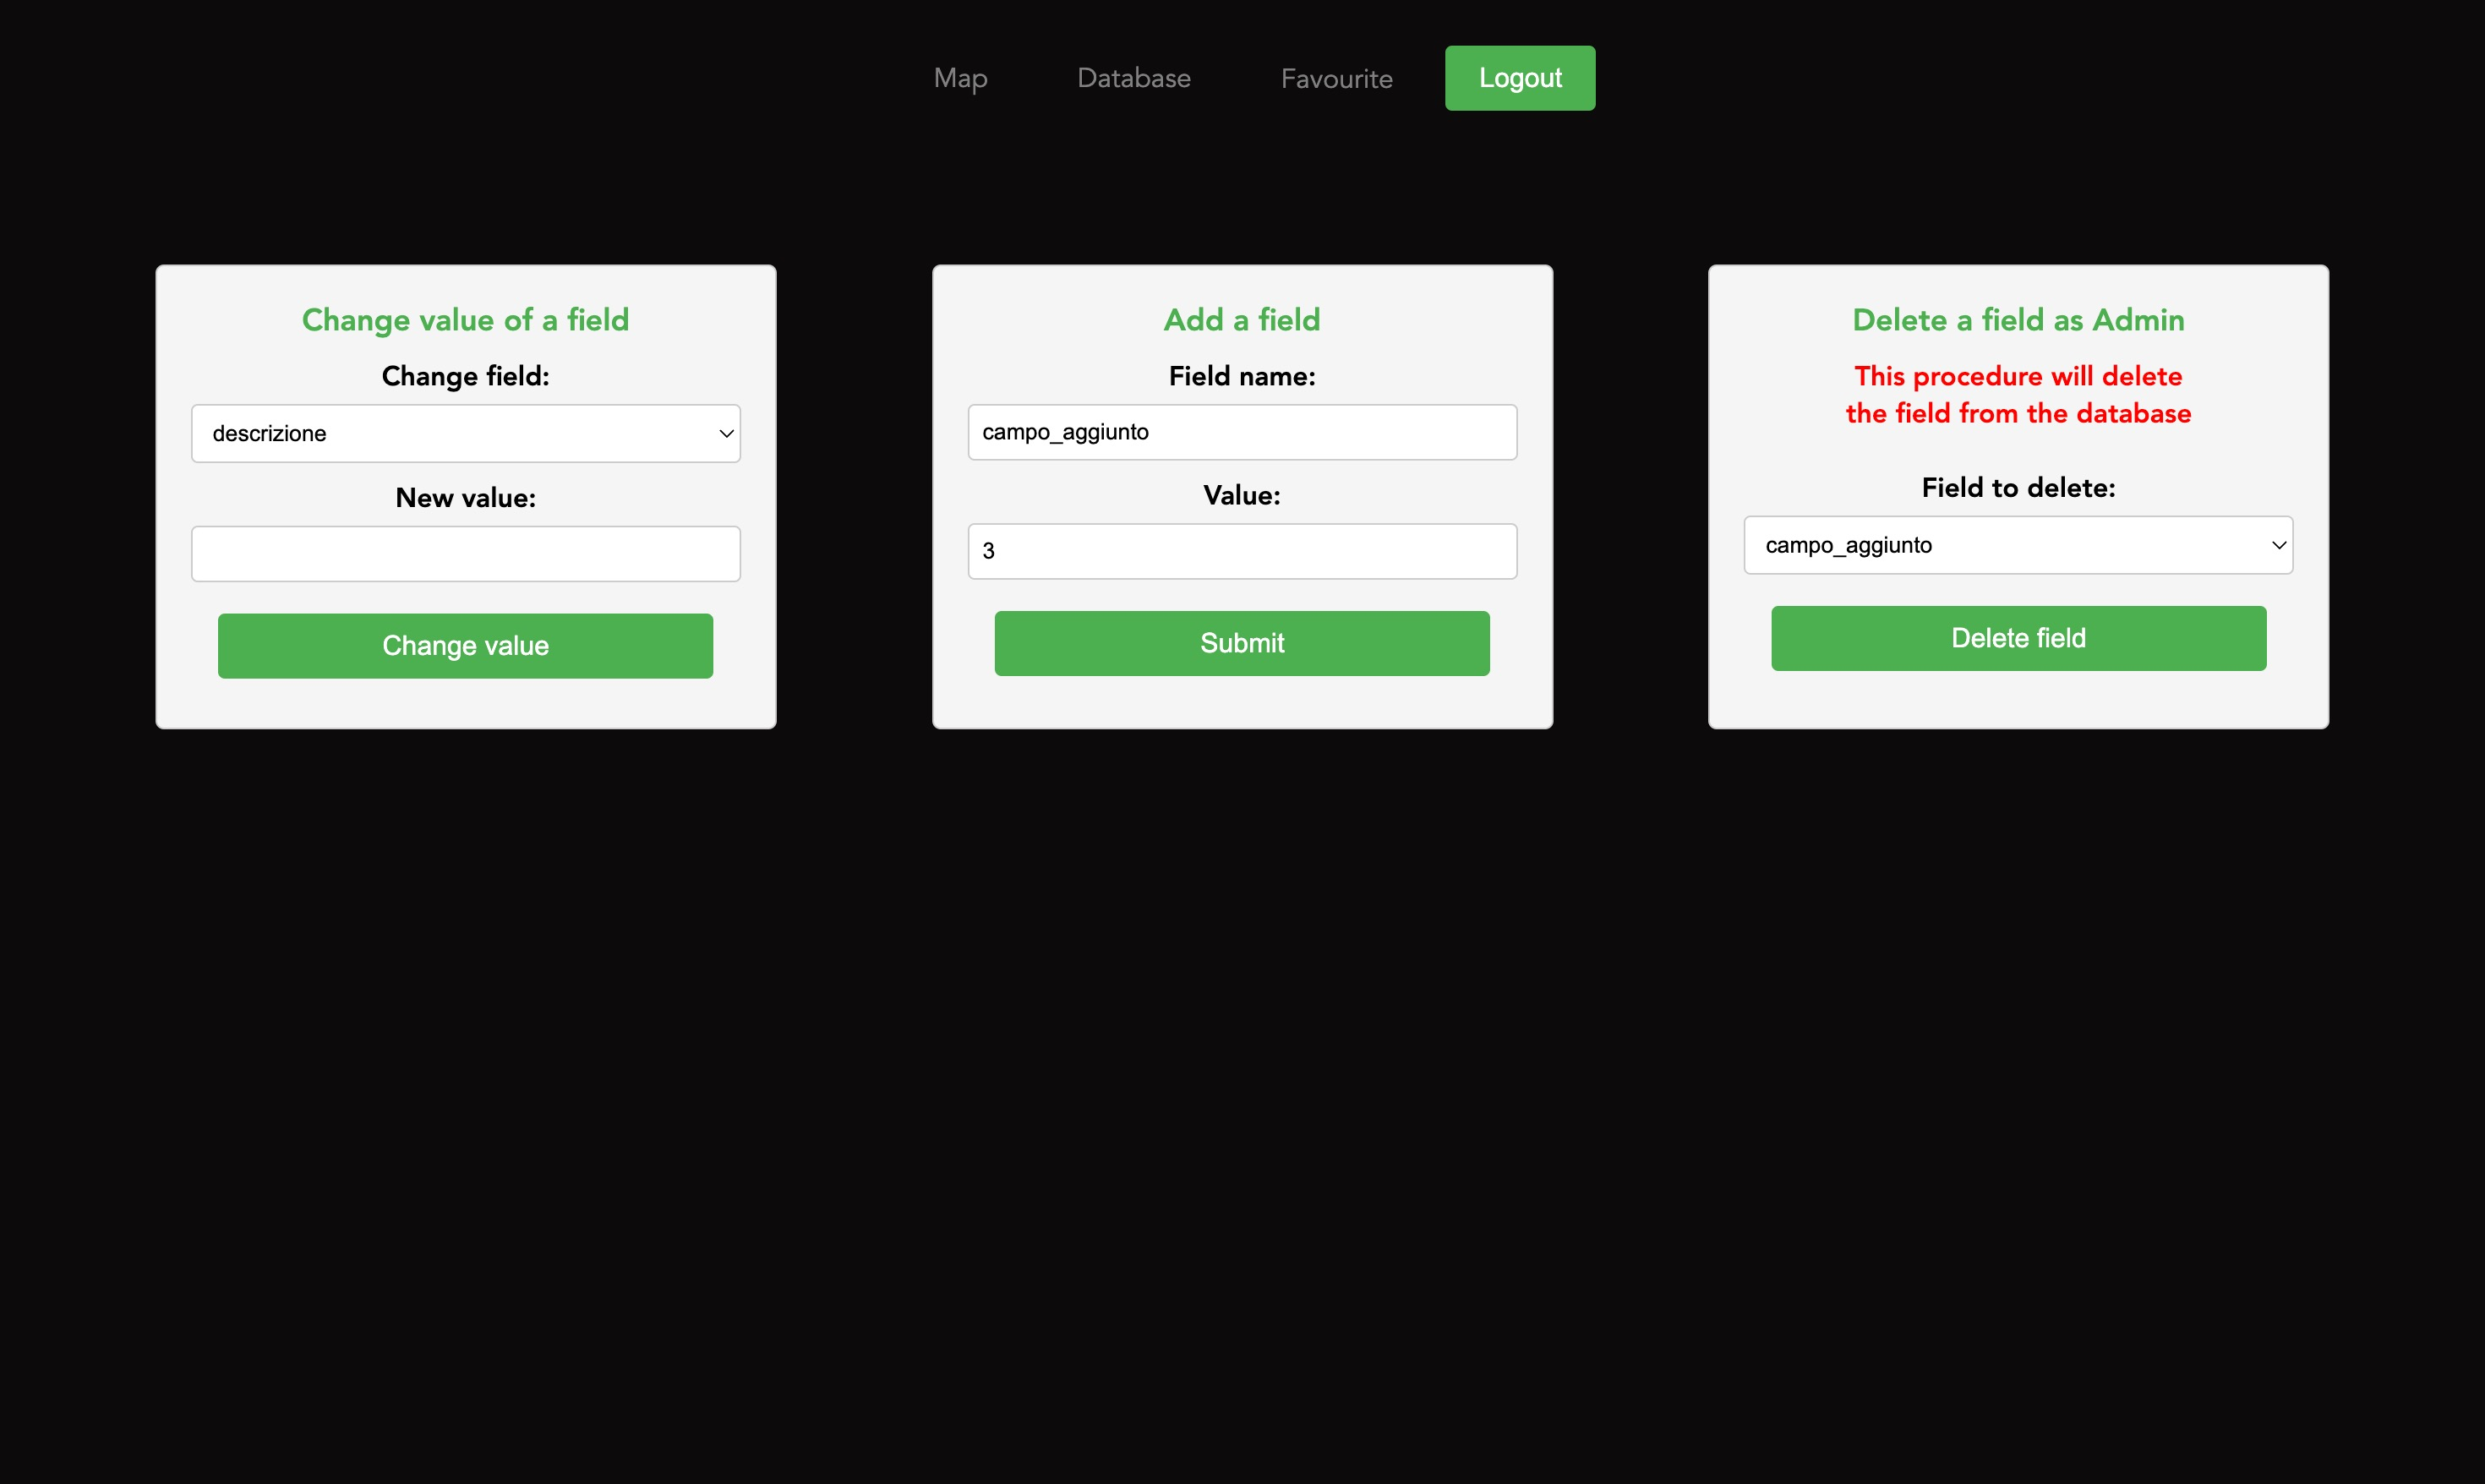
\includegraphics[width=13cm]{images/Extra_field.jpg}
\caption[Pagina per aggiungere informazioni sui punti di interesse]{Pagina per aggiungere informazioni sui punti di interesse}\label{fig:extra_field}
\end{center}
\end{figure}

Questa pagina presenta tre opzioni:

\begin{itemize}
    \item Cambiare valore ad un campo

    Selezionando un campo dal menù a tendina è possibile cambiarne il valore. Questa funzione è utilizzabile per tutti gli utenti.

    \item Aggiungere un campo

    È possibile aggiungere un campo a quel punto di interesse mettendogli il nome nella prima casella e il valore nella seconda. Nel caso verrà inserito un campo già presente nel punto, il valore di questo verrà sovrascritto. Questa funzione è utilizzabile per tutti gli utenti.

    \item Eliminare un campo

    È possibile eliminare un campo aggiunto dagli utenti dal punto di interesse. Questa funzione è utilizzabile solo per gli amministratori.
\end{itemize}

	

	%%%%%%%%%%%%%%%%%%%%%%%%%
	% inizio parte finale del documento
	%
	% eventuali appendici, bibliografia obbligatoria,
	% eventuale lista delle tabelle e delle figure (nel caso decommentare 
	% la riga con i comandi \listoffigures e \listoftables)
	%%%%%%%%%%%%%%%%%%%%%%%%%
	
    %%%%%%%%%%%%%%%%%%%%%%%%%%%%%%%%%%%%%%%%%non numera l'ultima pagina sinistra
\clearpage{\pagestyle{empty}\cleardoublepage}
%%%%%%%%%%%%%%%%%%%%%%%%%%%%%%%%%%%%%%%%%per fare le conclusioni
\chapter*{Conclusioni}
%%%%%%%%%%%%%%%%%%%%%%%%%%%%%%%%%%%%%%%%%imposta l'intestazione di pagina
\rhead[\fancyplain{}{\bfseries
CONCLUSIONI}]{\fancyplain{}{\bfseries\thepage}}
\lhead[\fancyplain{}{\bfseries\thepage}]{\fancyplain{}{\bfseries
CONCLUSIONI}}
%%%%%%%%%%%%%%%%%%%%%%%%%%%%%%%%%%%%%%%%%aggiunge la voce Conclusioni
                                        %   nell'indice
\addcontentsline{toc}{chapter}{Conclusioni} 
L'obiettivo di questo progetto di tesi è la realizzazione di un'applicazione web dedicata agli escursionisti nella regione Emilia-Romagna.

Sono stati esaminati i concetti di Digital Twin, Digital Shadow e Digital Thread, analizzandone prevalentemente le definizioni, l'origine e i vantaggi. Si è compreso il ruolo fondamentale del Digital Twin nell'Industria 4.0, del Digital Shadow nella raccolta dei dati degli utenti e del Digital Thread nella gestione continua delle informazioni.
Sono state analizzate le tecnologie fondamentali per lo sviluppo di questa piattaforma tra cui HTML, CSS, JavaScript e altre librerie e framework pertinenti. 
Infine sono state discusse le sfide tecniche affrontate durante lo sviluppo, focalizzandosi sulla visualizzazione dei percorsi escursionistici e sulla gestione dei dati. Sono state presentate le varie funzionalità dell'applicazione, tra cui la visualizzazione dei percorsi, i servizi di geo-localizzazione, la registrazione degli utenti e la possibilità di arricchire i dati relativi ai punti di interesse.

È importante notare che, mediante la modifica dei dati forniti per la creazione del database, è possibile estendere l'applicazione per consentire la visualizzazione di percorsi escursionistici in qualsiasi parte del mondo. Inoltre, siccome è già stata implementata la funzionalità di geo-localizzazione, potrebbe essere esplorata la possibilità di tracciare gli utenti lungo i percorsi e, potenzialmente, rendere possibile un'interazione tra gli escursionisti lungo lo stesso sentiero. Questi sviluppi futuri potrebbero ulteriormente trasformare l'applicazione in un social network dedicato agli amanti delle escursioni. In futuro potrebbero anche essere aggiunte integrazioni aggiuntive, usando i servizi offerti da \href{https://www.tripadvisor.com/}{\textit{Tripadvisor}}, da \href{https://www.google.com/maps/d/viewer?msa=0&iwloc=00044592e21a9f5590527&ved=0COIBEJwFSAE&sa=X&ei=I0ShTO3lOqiijQOHmtz6Aw&mid=1eLqvkQ9wGvMRVrAQsm5g7EdlnSY&ll=39.04394865349766,-76.85871&z=10}{\textit{Google places}} o da \href{https://www.arpae.it/it}{\textit{Arpae}}. Infine potrebbe essere aggiunta la possibilità di mostrare il meteo sulla regione o di mostrare le immagini satellitari riguardanti i punti di interesse.

\clearpage{\pagestyle{empty}\cleardoublepage}
    %\clearpage{\pagestyle{empty}\cleardoublepage}

\cleardoublepage

\rhead[\fancyplain{}{\bfseries BIBLIOGRAFIA}]{\fancyplain{}{\bfseries\thepage}}
\lhead[\fancyplain{}{\bfseries\thepage}]{\fancyplain{}{\bfseries BIBLIOGRAFIA}}
%%%%%%%%%%%%%%%%%%%%%%%%%%%%%%%%%%%%%%%%% aggiunge l'intestazione di pagina
%\chapter*{Bibliografia}


\phantomsection


\addcontentsline{toc}{chapter}{Bibliografia}
%%%%%%%%%%%%%%%%%%%%%%%%%%%%%%%%%%%%%%%%% aggiunge la voce Bibliografia nell'indice





\bibliography{backMatter/biblio}{}
\bibliographystyle{plain}


    % \rhead[\fancyplain{}{\bfseries \leftmark}]{\fancyplain{}{\bfseries
\thepage}}
%%%%%%%%%%%%%%%%%%%%%%%%%%%%%%%%%%%%%%%%%aggiunge la voce Bibliografia
                                        %   nell'indice

%%%%%%%%%%%%%%%%%%%%%%%%%%%%%%%%%%%%%%%%%non numera l'ultima pagina sinistra
\clearpage{\pagestyle{empty}\cleardoublepage}
\chapter*{Ringraziamenti}
\thispagestyle{empty}

\addcontentsline{toc}{chapter}{Ringraziamenti}

Qui possiamo ringraziare il mondo intero!!!!!!!!!!\\
Ovviamente solo se uno vuole, non \`e obbligatorio.
	
		
	%\input{./Appendice/appendice.tex}
	%%\clearpage{\pagestyle{empty}\cleardoublepage}

\cleardoublepage

\rhead[\fancyplain{}{\bfseries BIBLIOGRAFIA}]{\fancyplain{}{\bfseries\thepage}}
\lhead[\fancyplain{}{\bfseries\thepage}]{\fancyplain{}{\bfseries BIBLIOGRAFIA}}
%%%%%%%%%%%%%%%%%%%%%%%%%%%%%%%%%%%%%%%%% aggiunge l'intestazione di pagina
%\chapter*{Bibliografia}


\phantomsection


\addcontentsline{toc}{chapter}{Bibliografia}
%%%%%%%%%%%%%%%%%%%%%%%%%%%%%%%%%%%%%%%%% aggiunge la voce Bibliografia nell'indice





\bibliography{backMatter/biblio}{}
\bibliographystyle{plain}


	
	\nocite{*}

	%\cleardoublepage
	%\addcontentsline{toc}{chapter}{Bibliografia}


	
	%\listoffigures
	%\listoftables


\end{document}
